% -----------------------------------------------------------------
% Vorlage fuer Ausarbeitungen von
% Bachelor- und Masterarbeiten am ISS
% 
% Template for written reports or master theses at the ISS
% 
% For use with compilers pdflatex or latex->dvi2ps->ps2pdf.
%
% -----------------------------------------------------------------
% README, STUDENT USERS:
% We highly appreciate students using this template _AS IS_,period. 
% The document provides adjustable document preferences, 
% student information settings and typography definitions. Look for
% code delimited by *** ***
%
% The short explanation: it's the ISS common standard and 
% 	it's battle tested.
% The long explanation: 
%	We do not want you to go through the document and tweak the 
%	package options, layout parameters and line skips here and 
%	there and waste hours. We are providing this template such 
%	that you can fully concentrate on filling in the much more 
%	important _contents_ of your thesis.
%
% If you have serious needs on extra packages or design 
% modifications, talk to your supervisor _before_ modifying 
% the template.
% Similarly, we're happy if you give your supervisor a hint on any 
% errors in this template.
%
% -----------------------------------------------------------------
% History:
% Jan Scheuing,   04.03.2002
% Markus Buehren, 20.12.2004
% last changes:   10.01.2008 (removed unused packages), 
% 		07.08.2009 (added IEEEtran_LSS.bst file)
% 		02.05.2011 removed matriculation number from cover page
% Martin Kreissig, 25.01.2012: all eps/ps parts removed for 
% 				pdflatex to work properly
% Peter Hermannstaedter, 14.08.2012: fusion of versions for 
% 		latex/dvi/ps/pdf and pdflatex, additional comments,
% 		unification of document flags and student options
% Florian Liebgott, 12.03.2015: bug fixes, removal of obsolete options,
%		switch to UTF-8
% Florian Liebgott, 20.05.2015: fixed encoding problem on title page
% Florian Liebgott, 24.01.2017: changed deprecated font commands (like
%		\sl) to up-to-date commands to be compatible with
%		current TeX distributions.
% Felix Wiewel, 30.08.2021: Replace obsolete scrpage2 with scrlayer-scrpage
%
% -----------------------------------------------------------------
% If you experience any errors caused by this template, please
% contact Florian Liebgott (florian.liebgott@iss.uni-stuttgart.de)
% or your supervisor, so we can fix the errors.
% -----------------------------------------------------------------

\documentclass[12pt,DIV14,BCOR12mm,a4paper,footinclude=false,headinclude,parskip=half-,twoside,openright,cleardoublepage=empty,toc=index,bibliography=totoc,listof=totoc]{scrreprt}
% encoding needs to be defined here, otherwise umlauts on the titelpage won't work.
\usepackage[utf8]{inputenc}
%
%
%
% *****************************************************************
% -------------------> document preferences here <-----------------
% *****************************************************************
% Uncomment the settings you like and comment the settings you don't
% like.

% Language: 
% affects generic titles, Figure term, titlepage and bibliography
% (Note:if you switch the language, compile tex and bib >2 times)
\def \doclang{english} 	% For theses/reports in English
%def \doclang{german} 		% For theses/reports in German

% Hyperref links in the document:
\def \colortype{color} % links with colored text
%\def \colortype{bw} 	% plain links, standard text color (e.g. for print)
%\def \colortype{boxed} % links with colored boxes
% *****************************************************************
%
%
%
% *****************************************************************
% --------------> put student information here <------------------
% *****************************************************************
% Please fill in all items denoted by "to be defined (TBD)"
\def \deworktitle{}        % German title/translation
\def \enworktitle{Generation and Evaluation of Synthetic Test Images in an Industrial Context}        % English title/translation
\def\tutor{Dominik Track, M. Sc.\newline Martin Wimpff, M. Sc.\newline Prof. Dr.-Ing. Bin Yang}
\def \student{Swathi Kumar}
\def \worksubject{Masterarbeit D1501}  % type and number (S/Dxxxx) of your thesis
\def \startdate{22.04.2024}
\def \submission{22.10.2024}
\def \signagedate{22.10.2024}   % Date of signature of declaration on last page
\def \keywords{Synthetic Image Generation\newline Generative Models\newline Anomaly Detection}
\def \abstract{}

% *****************************************************************
%


\usepackage{amsmath}
\usepackage{amsfonts}
\usepackage{ifthen}
\ifthenelse{\equal{\doclang}{german}}{
	\usepackage[ngerman]{babel} %german version
	\def \maintitle{\deworktitle}
	\def \translatedtitle{\enworktitle}
	% set , to decimal and . to thousands separator, if German language is used
	\DeclareMathSymbol{,}{\mathord}{letters}{"3B}
	\DeclareMathSymbol{.}{\mathpunct}{letters}{"3A}
	}{
	%english version
	\def \maintitle{\enworktitle}
	\def \translatedtitle{\deworktitle}
	}
\usepackage{txfonts} % Times-Fonts
\usepackage[T1]{fontenc}
\usepackage{color}
\usepackage[headsepline]{scrlayer-scrpage} % Headings
\usepackage{cite}
\usepackage{subcaption}
\usepackage{tikz}
\usepackage{longtable}
\usepackage{tabularx}
\usetikzlibrary{positioning} % Load the positioning library
\usepackage{graphicx}
\usepackage{float}
\usepackage[format=hang]{caption}       % for hanging captions
\usepackage{subfig}                     % for subfigures
\usepackage{wrapfig}                    % for figures floating in text, alternatively you can use >>floatflt<<
\usepackage{booktabs}                   % nice looking tables (for tables with ONLY horizontal lines)

%%%%% Tikz / PGF - drawing beautiful graphics and plots in Latex
% \usepackage{tikz}
% \usetikzlibrary{plotmarks}              % larger choice of plot marks
% \usetikzlibrary{arrows}                 % larger choice of arrow heads
% % ... insert other libraries you need
% \usepackage{pgfplots}
% % set , to decimal and . to thousands separator for plots, if German language is used
% \ifthenelse{\equal{\doclang}{german}}{
% \pgfkeys{/pgf/number format/set decimal separator={,}}
% \pgfkeys{/pgf/number format/set thousands separator={.}}
% }{}
%%%%%%

\ifthenelse{\equal{\colortype}{color}}{
	% colored text version:
	\usepackage[colorlinks,linkcolor=blue]{hyperref}
	\newcommand{\bugfix}{\color{white}{\texttt{\symbol{'004}}}} % Bug-Fix Umlaute in Verbatim
}{
	\ifthenelse{\equal{\colortype}{boxed}}{
		% colored box version:
		\usepackage{hyperref}
		\newcommand{\bugfix}{\color{white}{\texttt{\symbol{'004}}}} % Bug-Fix Umlaute in Verbatim
	}{
		% monochrome version:
		\usepackage[hidelinks]{hyperref}
		\newcommand{\bugfix}{\color{white}{\texttt{\symbol{'004}}}} % Bug-Fix Umlaute in Verbatim
	}
}

% Layout and Headings
\pagestyle{scrheadings}
\automark{chapter}
\clearscrheadfoot
\lehead[]{\pagemark~~\headmark}
\rohead[]{\headmark~~\pagemark}
\renewcommand{\chaptermark}[1]{\markboth {\normalfont\slshape \hspace{8mm}#1}{}}
\renewcommand{\sectionmark}[1]{\markright{\normalfont\slshape \thesection~#1\hspace{8mm}}}
\addtolength{\textheight}{15mm}
\parindent0ex
\setlength{\parskip}{5pt plus 2pt minus 1pt}
\renewcommand*{\pnumfont}{\normalfont\slshape} % Seitenzahl geneigt
\renewcommand*{\sectfont}{\bfseries} % Kapitelueberschrift nicht Helvetica

% Settings for PDF document
\pdfstringdef \studentPDF {\student} 
\pdfstringdef \worktitlePDF {\maintitle}
\pdfstringdef \worksubjectPDF {\worksubject}
\hypersetup{pdfauthor=\studentPDF, 
            pdftitle=\worktitlePDF,
            pdfsubject=\worksubjectPDF}

% Title page
\titlehead{
	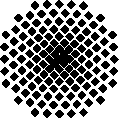
\includegraphics[width=20mm]{university-logo}
	\hspace{6mm}
	\ifthenelse{\equal{\doclang}{german}}{
		\begin{minipage}[b]{.6\textwidth}
		{\Large Universit\"at Stuttgart } \\
		Institut f\"ur Signalverarbeitung und Systemtheorie\\
		Professor Dr.-Ing. B. Yang \vspace{0pt}
		\end{minipage}
	}{
		\begin{minipage}[b]{.6\textwidth}
		{\Large University of Stuttgart } \\
		Institute for Signal Processing and System Theory\\
		Professor Dr.-Ing. B. Yang \vspace{0pt}
		\end{minipage}
	}
	\hspace{1mm}
	
\includegraphics[width=28mm]{isslogocolor}
}
\subject{\worksubject\vspace*{-5mm}} % Art und Nummer der Arbeit
\title{\maintitle}%\\ \Large{\subtitle}}
\subtitle{\translatedtitle}
\author{
\large
  \ifthenelse{\equal{\doclang}{german}}{
  \begin{tabular}{rp{7cm}}
    \Large 
    Autor:      & \Large \student \vspace*{2mm}\\
    Ausgabe:    & \startdate \\
    Abgabe:     & \submission \vspace*{3mm}\\
    Betreuer:   & \tutor \vspace*{2mm}\\
    Stichworte: & \keywords
  \end{tabular}
  }{
  \begin{tabular}{rp{7cm}}
    \Large 
    Author:             & \Large \student \vspace*{2mm}\\
    Date of work begin: & \startdate \\
    Date of submission: & \submission \vspace*{3mm}\\
    Supervisor:         & \tutor \vspace*{2mm}\\
    Keywords:           & \keywords
  \end{tabular}
  }
  \bugfix
}
\date{}
\publishers{\normalsize
  \begin{minipage}[t]{.9\textwidth}
    \abstract
Images captured in production environments exhibit various camera influences that the anomaly detector must learn to recognize. Without training on such diverse conditions, the detector is prone to misclassification and reduced performance. This master's thesis focuses on generating and evaluating synthetic test images to enhance the performance of these anomaly detectors in industrial contexts. Generative models, including Cycle-Consistent Generative Adversarial Network (CycleGAN) was used to generate synthetic images by transforming optimal setup images to include bad camera influences and Stable Diffusion to generate synthetic images directly from real images. The quality and similarity of these synthetic images were evaluated through various metrics to ensure their effectiveness. The performance of the anomaly detector was evaluated through different training approaches. The results demonstrated a significant reduction in false positives when trained with images (both real and synthetic) that included those camera influences.
  \end{minipage}
}

\numberwithin{equation}{chapter} 
\sloppy 

%
%
%
% *****************************************************************
% --------------> put typography definitions here <----------------
% *****************************************************************
% colors
\definecolor{darkblue}{rgb}{0,0,0.4}

% declarations
\newcommand{\matlab}{\textsc{Matlab}\raisebox{1ex}{\tiny{\textregistered}} }
% Integers, natural, real and complex numbers
\newcommand{\Z}{\mathbb{Z}}
\newcommand{\N}{\mathbb{N}}
\newcommand{\R}{\mathbb{R}}
\newcommand{\C}{\mathbb{C}}
% expectation operator
\newcommand{\E}{\operatorname{E}}
% imaginary unit
\newcommand{\im}{\operatorname{j}}
% Euler's number with exponent as parameter, e.g. \e{\im\omega}
\newcommand{\e}[1]{\operatorname{e}^{\,#1}}
% short command for \operatorname{}
\newcommand{\op}[1]{\operatorname{#1}}

% unknown hyphenation rules
\hyphenation{Im-puls-ant-wort Im-puls-ant-wort-ko-ef-fi-zien-ten
Pro-gramm-aus-schnitt Mi-kro-fon-sig-nal}
% *****************************************************************
%
\begin{document}

% title and table of contents
\pagenumbering{alph}
\maketitle
%\cleardoublepage
\pagenumbering{roman} % roman numbering for table of contents
\tableofcontents
\cleardoublepage
\setcounter{page}{1}
\pagenumbering{arabic} % arabic numbering for rest of document

% *****************************************************************
% -------------------> start writing here <------------------------

\chapter{Introduction}
\section{Motivation}
Deep learning models thrive on large volumes of data, as vast and diverse datasets are essential for training algorithms that achieve high accuracy and generalization~\cite{r1}. The performance of these models improves significantly with more data, allowing them to learn complex patterns and make more reliable predictions. However, acquiring such extensive datasets often presents significant challenges. Traditional data collection methods, especially in industrial settings can be costly, time-consuming, and impractical, if not impossible. Manual data annotation adds another layer of complexity, requiring considerable human effort and expertise. This creates a bottleneck in developing robust machine learning systems that require extensive, varied, and well-labelled data.

To overcome these challenges, synthetic data has emerged as a powerful alternative. Synthetic data is artificially generated by AI algorithms trained on real datasets, aiming to replicate the statistical properties and patterns of the original data~\cite{r2}. By modeling the probability distribution of real data and sampling from it, synthetic data generation creates new datasets that retain similar characteristics and predictive power as the original data. This method enables the rapid creation of large, diverse datasets, including rare or difficult-to-capture scenarios, thus addressing the limitations of traditional data collection. As a result, synthetic data facilitates more efficient model development and training, enabling better generalization and performance of machine learning systems.

\section{Problem Statement and Objectives}
In industrial environments, anomaly detection systems are crucial for ensuring production efficiency and quality. However, these detectors often fail to reliably distinguish between defective and non-defective products when they are not trained with enough images that capture real-world variations, such as brightness, shadowing, reflections, and distortions. Without exposure to these variations during training, the detectors may misclassify normal products affected by such influences as defective, even though they are not true anomalies. This underscores the importance of training data that reflects the diverse conditions found in actual production setups.

The objective of this thesis is to enhance the accuracy and robustness of an anomaly detector by providing it with synthetically generated images that incorporate different influences. Since collecting sufficient real images to represent the full spectrum of possible influences is often time-consuming and impractical, this approach aims to reduce the reliance on extensive real-world data, by using two different generative models to create realistic synthetic data that accurately replicate these artifacts. The generated synthetic images will then be evaluated using various metrics to assess their quality and similarity to real images before being integrated into the training dataset for the anomaly detector. By training the anomaly detector on this comprehensive dataset, the goal is to improve its ability to distinguish between genuine defects and normal variations caused by different camera effects.

\section{Outline}

The introduction provides a comprehensive overview of the significance of synthetic image generation in enhancing the efficacy of anomaly detection systems within industrial contexts, outlining the motivation and objectives of the research. Chapter~\ref{chapter2} provides essential theoretical foundations related to deep learning and anomaly detection, starting with an overview of deep learning principles and a comparison of discriminative and generative models. It further explores synthetic image generation techniques, focusing on Generative Adversarial Networks (GANs), particularly CycleGAN, and diffusion models, while also discussing the role of autoencoders in anomaly detection. In Chapter~\ref{chapter3}, the materials and methods are detailed, describing the datasets utilized, including the Nuts, Candles, BNI, and PCB datasets. This chapter also outlines the methodologies for generating synthetic images using CycleGAN and Stable Diffusion, alongside the evaluation metrics employed to assess image quality and the anomaly detection system's setup. Chapter~\ref{chapter4} presents the experimental results from CycleGAN and Stable Diffusion, including the results of evaluation metrics. It concludes by analyzing the impact of synthetic images on the performance of the anomaly detector, highlighting a significant reduction in false positives. Finally, Chapter~\ref{chapter5} summarizes the thesis's key findings, discussing its contributions to the field of anomaly detection and offering recommendations for future research directions that highlight the potential of synthetic data in industrial applications.

\chapter{Theoretical Background}
\label{chapter2}
This section introduces key concepts essential for understanding the generation of synthetic data and its application in anomaly detection. It begins with deep learning, a powerful method that allows models to learn complex patterns from large datasets. A distinction is drawn between discriminative models, which classify data based on learned patterns, and generative models, which produce new data resembling the original dataset. Key generative approaches, such as GANs and Diffusion Models, are covered, with a focus on CycleGAN (a conditional GAN) and Stable Diffusion, both of which are central to generating synthetic images. The significance of synthetic data in overcoming challenges related to data scarcity and variability is discussed, along with an overview of anomaly detection techniques, crucial for identifying deviations from expected patterns in industrial applications.
\section{Deep Learning}
Deep learning, a branch of machine learning, employs deep neural networks, which are multilayered architectures designed to emulate the intricate decision-making capabilities of the human brain. This approach underpins many of the artificial intelligence (AI) applications prevalent in today’s technology~\cite{wuttke2024}.

Neural networks, or artificial neural networks (ANN), are designed to mimic the human brain by using interconnected layers of nodes (neurons) that process information in a similar manner. These nodes are associated with weights and biases, which influence the input data to make accurate predictions or classifications. This structure allows neural networks to identify and interpret intricate patterns in data, making them versatile tools for various tasks involving detailed analysis and decision-making~\cite{hardesty2017explained}.

Deep neural networks (DNN) consist of multiple layers, where each layer builds on the previous one to refine and optimize the predictions. This process, known as \textbf{forward propagation} , involves passing data through the input layer, where the deep learning model ingests the data, and through a series of hidden layers that apply transformations~\cite{luhaniwal2019}. The final output layer produces the prediction or classification. Each layer extracts progressively more abstract features from the data, enabling deep learning models to understand intricate patterns in images, such as shapes, textures, and complex structures.

To improve the model's accuracy, a process called \textbf{backpropagation} is used. Backpropagation calculates the error between the predicted output and the actual target value, using algorithms like gradient descent to adjust the weights and biases of the network. By iteratively updating these parameters through the layers, the model learns to minimize errors and improve performance~\cite{rumelhart1986learning}. Over time, this combination of forward propagation and backpropagation enables the neural network to make increasingly accurate predictions.
\section{Discriminative Vs. Generative Models}
In machine learning, models are often categorized into two broad types: discriminative models and generative models. Understanding the distinction between these two approaches is crucial for selecting the appropriate model for specific tasks, such as classification or data generation.

\begin{figure}
	\centering
	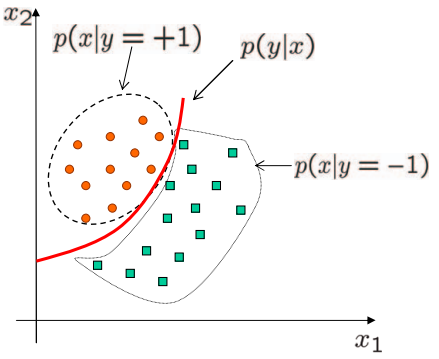
\includegraphics[scale=.7]{../media/Discriminative Vs Generative.PNG}
	\caption{Comparison of generative and discriminative models. Discriminative models concentrate on identifying the boundaries that separate different classes, whereas generative models are centered on producing data within each class\cite{tu2007learning}}
	\label{disc_vs_gen}
\end{figure}

\subsection{Discriminative Models}
Given a training dataset consisting of data points \(X\) and their corresponding labels \(Y\), a discriminative model learns the conditional probability distribution \(P(Y | X)\)~\cite{deng2016deep}. This model focuses on modelling the decision boundary between classes, directly learning the mapping from input data \(X\)  to the output labels \(Y\). The goal is to find the best function that can separate or classify the data points based on their features. By estimating \(P(Y | X)\), the model can predict the class of new data points by determining which class label has the highest probability given the input features.

Discriminative models are particularly useful in classification and regression tasks where the objective is to assign a label or a continuous value to each data point based on learned patterns and features~\cite{wikipedia2024}. These models do not attempt to model the underlying distribution of the data but rather focus on the decision boundaries between different classes.

\begin{figure}
	\centering
	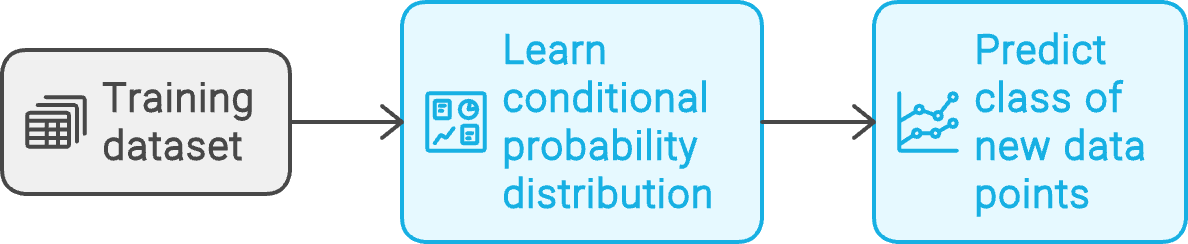
\includegraphics[scale=.3]{../media/Discriminative_model.png}
	\caption{Discriminative Model Workflow~\cite{Nanda:2024}}
	\label{disc}
\end{figure}

\subsection{Generative Models}
Generative models aim to learn the underlying distribution of a dataset in order to generate new data points that resemble the original data. Given a training dataset of data points \( X \) and their corresponding labels \( Y \), a generative model learns the joint probability distribution \( P(X, Y) \) or the conditional distribution \( P(Y|X) \)~\cite{deng2016deep}. By modeling the data in this way, the model can generate new samples that share characteristics with the training data, which is useful for tasks like data augmentation and simulation~\cite{zheng2023toward}. While generative models are primarily designed for tasks like data synthesis and simulation, they can also be used for discrimination by applying Bayes’ rule~\cite{ng2001discriminative}: 
\begin{equation}
P(Y|X) = \frac{P(X, Y)}{P(X)}
\end{equation}
However, this approach is rarely employed in practice, as discriminative models are typically more effective for classification tasks.
\begin{figure}
	\centering
	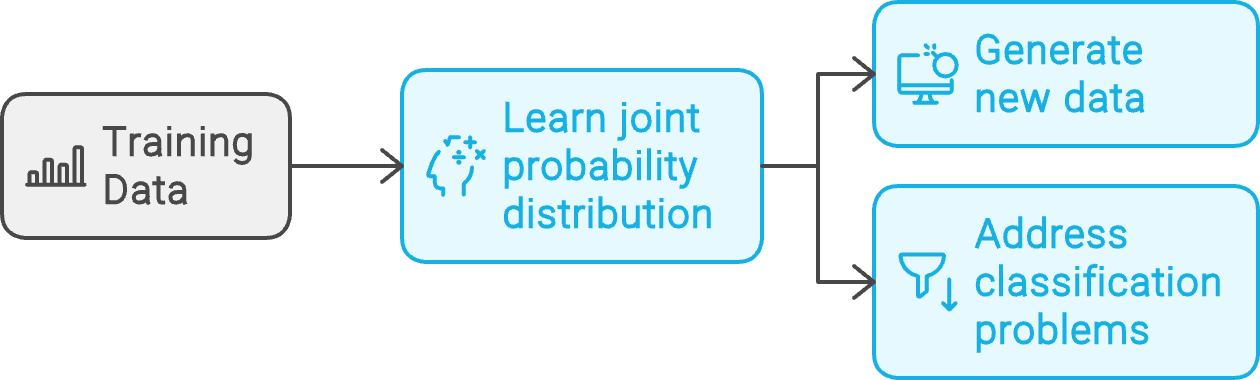
\includegraphics[scale=.3]{../media/Generative Model.png}
	\caption{Generative Model Workflow\cite{Nanda:2024}}
	\label{gen}
\end{figure}
Generative models are particularly valuable in scenarios where the goal is to understand the underlying data distribution or to generate new data samples. Unlike discriminative models, which focus solely on predicting or classifying data points, generative models attempt to model how the data was generated. This approach enables the creation of realistic synthetic data and is useful in applications such as image synthesis, data augmentation, and anomaly detection. By capturing the full distribution of the data, generative models provide a more comprehensive understanding of the data and its variations. Given that this thesis centers on synthetic image generation, generative models are fundamental to accomplishing this goal.
\section{Synthetic Image Generation}
Synthetic data refers to data that is artificially generated to replicate the statistical properties and underlying patterns of real-world data~\cite{raghunathan2021synthetic}. For training machine learning models, synthetic data is employed to augment or substitute real-world datasets, especially when obtaining real data is constrained by scarcity, cost, or privacy concerns. By utilizing advanced methods such as computer simulations and generative models, synthetic data can be produced in large volumes, encompassing a wide range of scenarios and variations. This approach not only facilitates the training and validation of models but also ensures that sensitive or proprietary information remains protected, while still providing the comprehensive and representative data needed for robust model performance.
\begin{figure}
	\centering
	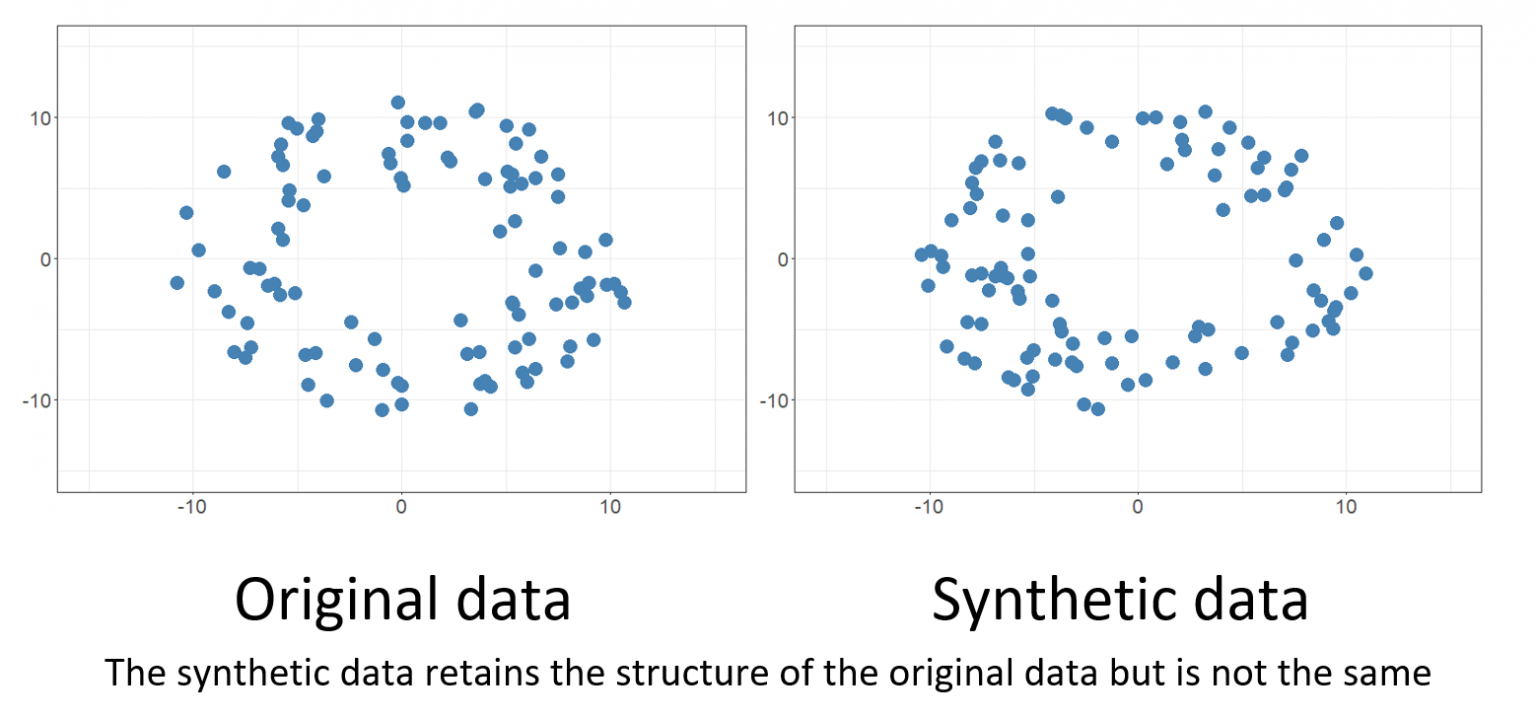
\includegraphics[scale=.3]{../media/synthetic_data_image-1536x718.png}
	\caption{The image shows two scatterplots: one of original data and one of synthetic data generated from the original data. The synthetic data retains the structure of the original data but is not the same. This is a common example of how generative models can be used to create new data that is similar to the original data, but not identical~\cite{Karen:2020}}
	\label{synthetic_data}
\end{figure}
In the context of image generation, synthetic images play an essential role in enhancing model training, especially for deep learning applications such as object detection, classification, and anomaly detection~\cite{anderson2022synthetic}. These images are generated to replicate specific features or conditions seen in real images but with the flexibility to introduce controlled variations. Synthetic images are commonly used to address challenges like data imbalance, variability in test conditions, or when acquiring real images is impractical or cost-prohibitive.

Generative models, such as Generative Adversarial Networks, Diffusion Models, and Variational Autoencoders (VAEs), are instrumental in the generation of synthetic images. GANs utilize a generator and a discriminator network in a competitive setting to create highly realistic images~\cite{schonfeld2022improving}. Diffusion Models work by progressively denoising random noise to generate coherent images, offering high fidelity and versatility~\cite{wang2023diffusion}. These models excel in generating high-quality synthetic images that closely mimic real data, which enhances model robustness and accuracy in handling varied scenarios. The following Chapters~\ref{sec:GANs_theory} and ~\ref{sec:diffusion_model_theory} will provide an in-depth examination of GANs and Diffusion Models, detailing their methodologies and applications in synthetic image generation.

On the other hand, Variational Autoencoders are another type of generative model that can produce synthetic images. While VAEs are effective at learning a compact latent representation of data and generating diverse samples, they often struggle with producing high-quality images with fine details. The images generated by VAEs can sometimes appear blurred or less realistic compared to those produced by GANs or Diffusion Models. This limitation makes VAEs less suitable for tasks requiring high-resolution and detailed synthetic images~\cite{cai2019multi}.
\section{Generative Adversarial Networks}
\label{sec:GANs_theory}
Generative Adversarial Networks, introduced by Goodfellow \textit{et al.} in 2014~\cite{goodfellow2014generative}, represent a powerful class of generative models. Central to GANs is the concept of \textbf{adversarial training}, which is inspired by Nash equilibrium in game theory. In this framework, two entities, the generator and the discriminator, engage in a competitive game. The generator's objective is to learn the distribution of real data and produce synthetic data that closely resembles it, while the discriminator's role is to distinguish between real and generated data. The game involves both entities continuously refining their strategies: the generator improves its ability to produce realistic data, and the discriminator enhances its accuracy in detecting fake data. This iterative process seeks to achieve a Nash equilibrium, where the generator's outputs are indistinguishable from real data according to the discriminator.
\begin{figure}
	\centering
	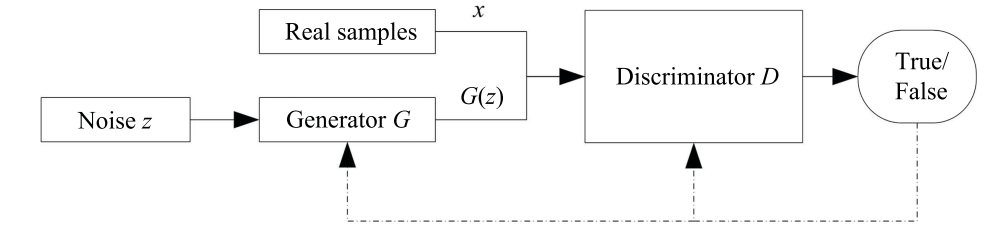
\includegraphics[scale=0.7]{../media/structure of GAN1.PNG}
	\caption{Structure of GAN~\cite{wang2017generative}}
	\label{GAN_struct}
\end{figure}
The structure of GAN is shown in Figure~\ref{GAN_struct}. Any differentiable function can be used as the generator and the discriminator. Here, we use differentiable functions \( D \) and \( G \) to represent the discriminator and the generator, and their inputs are real data x and random variables z, respectively. To learn the generator's distribution \( p_g\) over the data \( x \), we start by defining a prior distribution \( p_z(z) \) on the input noise variables. We then represent a mapping from the noise space to the data space using \( G(z; \theta_g) \), where \( G \) is a differentiable function modeled as a multilayer perceptron with parameters \( \theta_g \). Alongside, we define a second multilayer perceptron \( D(x; \theta_d) \) that outputs a single scalar. \( D(x) \) estimates the probability that \( x \) originates from the real data distribution rather than from \( p_g \). The discriminator \( D \) is trained to maximize the probability of correctly classifying both real data examples and samples generated by \( G \). Simultaneously, the generator \( G \) is trained to minimize \( \log(1 - D(G(z))) \)~\cite{wang2017generative}. 

This setup creates a two-player minimax game with the following value function \( V(G, D) \):
\begin{equation}
\min_{G} \max_{D} V(G, D) = \mathbb{E}_{x \sim p_{\text{data}}(x)} [\log D(x)] + \mathbb{E}_{z \sim p_z(z)} [\log(1 - D(G(z)))]
\end{equation}

Here, \( \mathbb{E} \) denotes the expectation over the respective distributions.

This framework captures the essence of \textbf{unconditional GANs}, where the primary focus is on learning the data distribution solely from random noise. In these models, the generator creates data samples based solely on the input noise \( z \) without additional context or control over the specific characteristics of the generated data. As a result, unconditional GANs are adept at learning the overall data distribution but lack the capability to control the generation of specific modes or attributes within the data~\cite{lee2022generator}.

To achieve more precise control over the generated data, \textbf{conditional GANs} utilize additional information to guide the data generation process. This approach, which enables targeted generation of data with specific attributes, will be discussed in the following section.

Several prominent unconditional GAN variants have made substantial contributions to the development of generative techniques. The original GAN, introduced by Goodfellow \textit{et al.}~\cite{goodfellow2014generative}, laid the groundwork for using adversarial training to generate realistic data from noise. The \textbf{Deep Convolutional GAN (DCGAN)}~\cite{radford2015unsupervised} enhanced this by incorporating convolutional layers in both the generator and discriminator, leading to improved image quality. The \textbf{Wasserstein GAN (WGAN)}~\cite{arjovsky2017wasserstein} addressed training instability by employing the Wasserstein distance as a loss metric, providing more stable and reliable convergence. The \textbf{Least Squares GAN (LSGAN)}~\cite{mao2017least} introduced the use of least squares loss instead of binary cross-entropy, which helps in achieving more stable training and high-quality images. Additionally, the \textbf{Progressive Growing GAN (PGGAN)}~\cite{karras2017progressive} introduced a technique of progressively increasing image resolution during training, significantly improving the quality of generated images. These developments in unconditional GANs have laid the foundation for more advanced models, including those that incorporate additional controls over the data generation process.

\subsection{Conditional GANs}
Conditional generative adversarial networks (cGANs) extend the traditional GAN architecture by conditioning both the generator and discriminator on additional information \( y \), which can include class labels, attributes, or other types of data. This conditioning allows the model to direct the generation process, enabling it to produce outputs that align with the given input condition. 
\begin{figure}
	\centering
	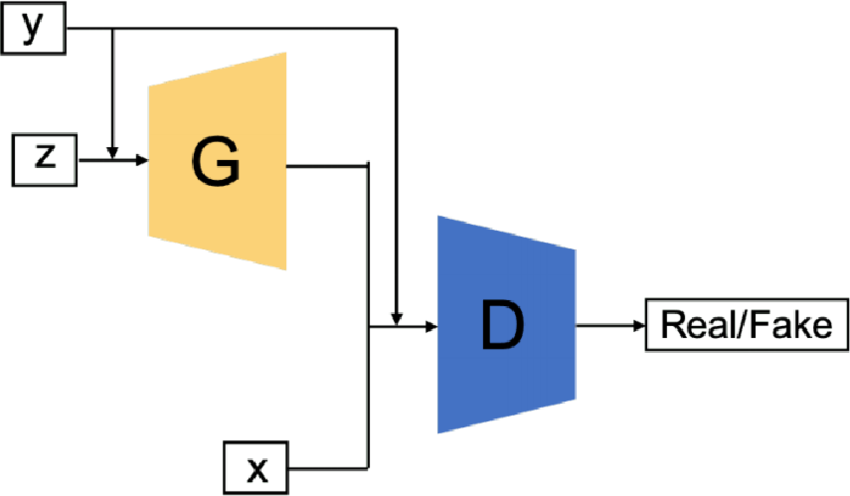
\includegraphics[scale=.9]{../media/Conditional-GAN-architecture.png}
	\caption{Conditional GAN architecture~\cite{eckerli2106generative}}
	\label{cGAN}
\end{figure}
In this setup, the generator receives both a noise vector \( z \) and the condition \( y \), combining them into a joint hidden representation to generate data. Meanwhile, the discriminator is provided with both the real or generated data \( x \) and the condition \( y \), aiming to assess whether the generated data matches the given condition.

The objective function of cGANs modifies the original GAN formulation as follows~\cite{gauthier2014conditional}:
\begin{equation}
\min_{G} \max_{D} V(D, G) = \mathbb{E}_{x \sim p_{\text{data}}(x)} [\log D(x|y)] + \mathbb{E}_{z \sim p_z(z)} [\log(1 - D(G(z|y)))]
\end{equation}

The incorporation of conditional information significantly enhances the adaptability of the GAN framework, making it particularly well-suited for tasks that require controlled outputs, such as \textbf{image-to-image translation}. In these scenarios, the model is tasked with transforming an image from one domain into another based on specific input conditions. By conditioning on auxiliary data, conditional GANs allow for finer control over the generated content, ensuring that the output aligns closely with the given input while maintaining high visual fidelity.

One widely recognized cGAN for image-to-image translation is \textbf{Pix2Pix}, introduced by Isola \textit{et al.} in 2017\cite{isola2017image}. This model is specifically trained on paired datasets, where each input image has a corresponding target image in the other domain. By conditioning the GAN on the input image, Pix2Pix enables the generator to learn the mapping between two domains, effectively translating an image from one domain to its target counterpart. The generator in Pix2Pix aims to produce outputs that match the target image, while the discriminator evaluates whether the generated image is the true paired image or a synthesized one. Through this adversarial process, Pix2Pix is highly effective in a wide range of image translation tasks, such as converting sketches to photographs\cite{sangkloy2017scribbler}, grayscale to color images, or even transforming satellite imagery into maps. However, Pix2Pix relies heavily on having paired training data, which limits its applicability in cases where paired data is scarce or unavailable.
\subsection{CycleGANs: Unpaired Image-to-Image Translation}
\textbf{Cycle-Consistent Generative Adversarial Networks} were introduced by Zhu \textit{et al.} in 2017. CycleGANs extend the concept of GANs to situations where paired training data is not available by leveraging unpaired datasets\cite{zhu2017unpaired}.

Unlike Pix2Pix, which requires paired images \((x_i, y_i)\) where \(x_i\) is an image from Domain A and \(y_i\) is its corresponding image in Domain B, CycleGANs work with two sets of unpaired images \(\{x_i\}\) from Domain A and \(\{y_i\}\) from Domain B.
\begin{figure}
	\centering
	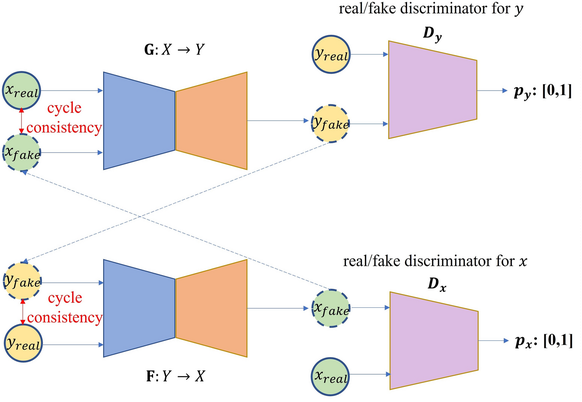
\includegraphics[scale=.7]{../media/Overview-of-CycleGAN-architecture.png}
	\caption{Overview of CycleGAN architecture\cite{article}}
	\label{cycleGAN}
\end{figure}
The CycleGAN framework consists of two generator networks \(G: \mathcal{X} \to \mathcal{Y}\) and \(F: \mathcal{Y} \to \mathcal{X}\), and two discriminator networks \(D_X\) and \(D_Y\). Here, \(G\) translates images from Domain A to Domain B, while \(F\) translates images from Domain B to Domain A. The discriminators \(D_X\) and \(D_Y\) aim to differentiate between real images and generated images in their respective domains.

The key innovation in CycleGANs is the cycle-consistency loss, which enforces that an image translated from Domain A to Domain B and then back to Domain A should approximately match the original image. This can be mathematically expressed as:

\begin{equation}
\mathcal{L}_{\text{cyc}}(G, F) = \mathbb{E}_{x \sim \mathcal{X}}[\|F(G(x)) - x\|_1] + \mathbb{E}_{y \sim \mathcal{Y}}[\|G(F(y)) - y\|_1]
\end{equation}

where \(\mathcal{L}_{\text{cyc}}\) denotes the cycle-consistency loss, \(\| \cdot \|_1\) represents the \(L_1\) norm, and \(\mathbb{E}\) denotes the expectation over the respective domains.

In addition to the cycle-consistency loss, CycleGANs use adversarial losses for each domain to ensure the generators produce outputs that are indistinguishable from real images. The adversarial losses can be defined as:

\begin{equation}
\mathcal{L}_{\text{adv}}(G, D_Y) = \mathbb{E}_{y \sim \mathcal{Y}}[\log D_Y(y)] + \mathbb{E}_{x \sim \mathcal{X}}[\log(1 - D_Y(G(x)))]
\end{equation}

\begin{equation}
\mathcal{L}_{\text{adv}}(F, D_X) = \mathbb{E}_{x \sim \mathcal{X}}[\log D_X(x)] + \mathbb{E}_{y \sim \mathcal{Y}}[\log(1 - D_X(F(y)))]
\end{equation}

where \(\mathcal{L}_{\text{adv}}(G, D_Y)\) and \(\mathcal{L}_{\text{adv}}(F, D_X)\) are the adversarial losses for the generators \(G\) and \(F\), and their respective discriminators \(D_Y\) and \(D_X\).

The total loss in the CycleGAN framework, combining the adversarial and cycle-consistency losses, can be expressed as:

\begin{equation}
L_{\text{CycleGAN}}(G, F, D_X, D_Y) = L_{\text{adv}}(G, D_Y) + L_{\text{adv}}(F, D_X) + \lambda_{\text{cyc}} L_{\text{cyc}}(G, F)
\end{equation}

Here, \(\lambda_{\text{cyc}}\) is a hyperparameter that adjusts the relative importance of the cycle-consistency loss. Training the CycleGAN involves solving the following optimization problem:

\begin{equation}
\min_{G, F} \max_{D_X, D_Y} L_{\text{CycleGAN}}(G, F, D_X, D_Y)
\end{equation}

In this min-max game, the generators \(G\) and \(F\) attempt to create convincing images that fool the discriminators \(D_Y\) and \(D_X\), while the discriminators are tasked with distinguishing real images from the ones generated by \(G\) and \(F\).

To further guide the generators to preserve the content of input images that are already in the target domain, an additional identity loss \(L_{\text{id}}\) is introduced:

\begin{equation}
L_{\text{id}}(G, F) = \mathbb{E}_{x \sim X} [\| G(x) - x \|_1] + \mathbb{E}_{y \sim Y} [\| F(y) - y \|_1]
\end{equation}

This identity loss encourages the generators to output images similar to the input when the input is already from the desired domain, helping to maintain the original characteristics of the images.
\section{Diffusion Models}
\label{sec:diffusion_model_theory}
The advent of diffusion models marks a major breakthrough in the domain of generative modeling, a field focused on learning the underlying data distribution and synthesizing new data points that resemble the original dataset. Early generative methods, such as Variational Autoencoders~\cite{VAE} and Generative Adversarial Networks~\cite{goodfellow2014generative}, laid the groundwork for modern generative approaches by leveraging probabilistic modeling and adversarial training, respectively. Despite their success, both VAEs and GANs exhibit limitations, VAEs often produce blurry outputs due to the variational approximation, while GANs are prone to issues such as mode collapse and instability during training. Diffusion models\cite{diffusion1,diffusion2} have emerged as a powerful alternative, offering a more stable and interpretable generative process. By modeling the data generation as a gradual denoising process, diffusion models can achieve high-quality sample generation with theoretically grounded stability, making them a robust alternative in modern generative tasks.

The modern framework of diffusion models was formalized by Ho \textit{et al.} (2020) with the introduction of \textbf{Denoising Diffusion Probabilistic Models (DDPM)}~\cite{diffusion2}. DDPM models the generative process as a \textbf{Markov chain} that progressively adds Gaussian noise to data in a series of discrete timesteps, forming a \textbf{forward diffusion process}. In this process, a data point \(\mathbf{x}_0\) is gradually transformed into a highly noisy version \(\mathbf{x}_T\) over \(T\) steps, according to the following Gaussian transition:

\begin{equation}
q(\mathbf{x}_t | \mathbf{x}_{t-1}) = \mathcal{N}(\mathbf{x}_t; \sqrt{\alpha_t} \mathbf{x}_{t-1}, (1 - \alpha_t)\mathbf{I})
\end{equation}

where \(\alpha_t\) is a variance schedule controlling the amount of noise added at each timestep \(t\). Figure \ref{forward} illustrates this \textbf{forward diffusion process}, where noise is progressively introduced to an original image.

\begin{figure}
	\centering
	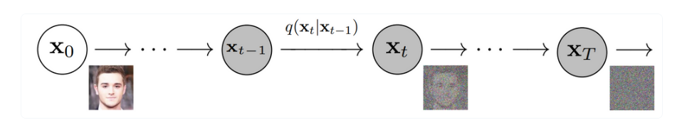
\includegraphics[scale=.9]{../media/diffusion_forward_process.png}
	\caption{The forward diffusion process: gradual noise addition to transform an image \(\mathbf{x}_0\) into \(\mathbf{x}_T\)~\cite{yainnoware2022}.}
	\label{forward}
\end{figure}

The core task of DDPM is to reverse this process by learning a generative model that reconstructs \(\mathbf{x}_0\) from \(\mathbf{x}_T\) by denoising in small, incremental steps. The \textbf{reverse diffusion process} is defined as:

\begin{equation}
p_\theta(\mathbf{x}_{t-1} | \mathbf{x}_t) = \mathcal{N}(\mathbf{x}_{t-1}; \mu_\theta(\mathbf{x}_t, t), \Sigma_\theta(\mathbf{x}_t, t))
\end{equation}

where \(\mu_\theta(\mathbf{x}_t, t)\) and \(\Sigma_\theta(\mathbf{x}_t, t)\) represent the mean and variance of the denoised image predicted by the neural network parameterized by \(\theta\). Figure \ref{reverse} shows how the reverse diffusion process works to denoise an image by iteratively reconstructing \(\mathbf{x}_0\) from \(\mathbf{x}_T\).

\begin{figure}
	\centering
	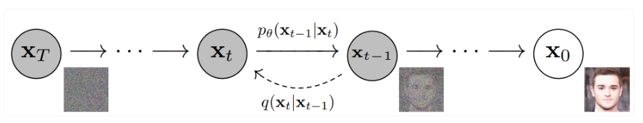
\includegraphics[scale=.9]{../media/diffusion_reverse_process.png}
	\caption{The reverse diffusion process: reconstructing the original image \(\mathbf{x}_0\) by denoising a noisy image \(\mathbf{x}_T\)~\cite{diffusion2}.}
	\label{reverse}
\end{figure}

This formulation allows DDPM to produce high-quality samples by reversing the noise addition process in a principled and stable manner. The introduction of DDPM has reignited interest in generative modeling, positioning diffusion models as a compelling alternative to Variational Autoencoders and Generative Adversarial Networks.

In early 2021, OpenAI introduced \textbf{DALL-E}~\cite{DALL_E} and \textbf{CLIP}~\cite{CLIP}, two landmark models that significantly advanced multimodal generative modeling. While DALL-E does not directly use diffusion processes, it laid the groundwork for subsequent models by employing a \textbf{Vision Transformer (ViT)}~\cite{ViT} to represent images as sequences of tokens. This tokenization allowed DALL-E to generate new images from a set of tokens, with textual tokens at the start of the sequence to condition the model on specific prompts. DALL-E's capacity to generate novel and imaginative images, such as the famous \emph{avocado armchair} shown in Figure~\ref{AvacadoArmchair} , showcased the potential of this approach. The model's outputs were further refined using \textbf{CLIP} (Contrastive Language-Image Pre-training), which pruned image candidates by evaluating their semantic alignment with the input text, thus functioning as an auto-cherry-picking mechanism.
\begin{figure}
	\centering
	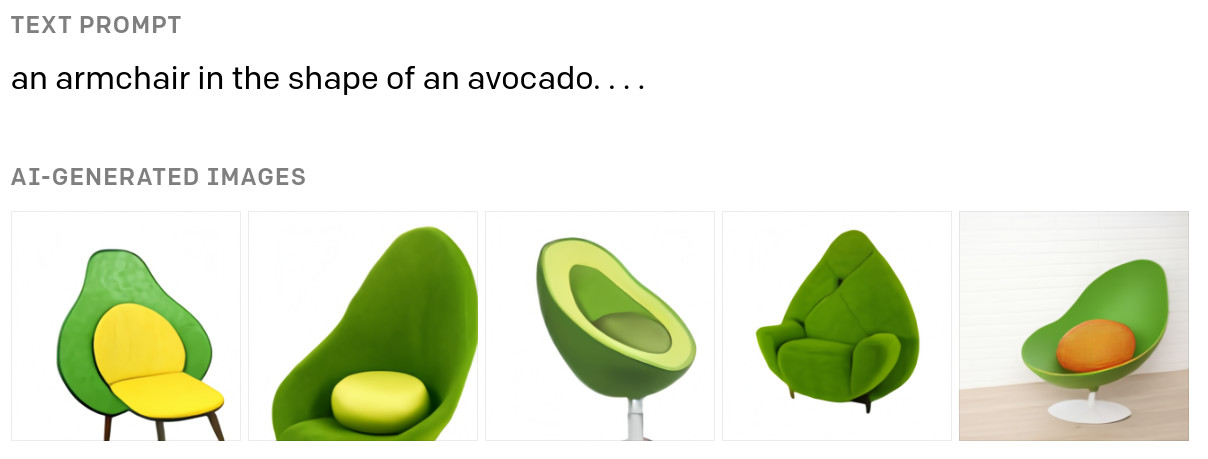
\includegraphics[scale=.3]{../media/DallE-AvacadoArmchair_1208x459.jpg}
	\caption{The famous Avocado chair (Prompt: ”an armchair in the shape of an avocado”)~\cite{openai2021}}
	\label{AvacadoArmchair}
\end{figure}

In early 2021, Nichol \& Dhariwal introduced an improved variant of Denoising Diffusion Probabilistic Models, focusing on enhancing the model's efficiency and image quality by refining the noise scheduling process\cite{Improved_denoising_diffusion}. Their work introduced a better timestep scheduler that adjusted the density of steps, making them denser toward the final stages of the image generation process. This change allowed the model to recover finer details in the generated images, reducing the number of steps required for high-quality outputs.

Later that year, in September 2021, Google introduced another significant advancement with \textbf{"Classifier-Free Diffusion Guidance"}, proposed by Ho \& Salimans \cite{ho2022classifier}. This method eliminated the need for external classifiers during the diffusion process by training the model with and without auxiliary information (such as class labels or text descriptions). During generation, the model computes the difference in outputs from both conditions, guiding the process and providing greater flexibility and control over the generated images. Classifier-free guidance became a crucial tool in improving diffusion-based models, further pushing the boundaries of generative modeling.

On December 20, 2021, two groundbreaking papers were released, marking a significant milestone in the development of diffusion models. The first, titled \textbf{"GLIDE: Towards Photorealistic Image Generation and Editing with Text-Guided Diffusion Models"}, was introduced by Nichol et al. \cite{nichol2021glide}. This model from OpenAI presented a novel approach to generating and editing images using textual prompts. GLIDE employed a text-guided diffusion model capable of producing photorealistic images, significantly advancing image generation technology. Moreover, it incorporated pre-trained 'filtered' models to mitigate harmful outputs, making it a practical tool for creative applications.

Simultaneously, Rombach \textit{et al.} from the Ommer Lab in Europe introduced \textbf{"High-Resolution Image Synthesis with Latent Diffusion Models,"} which brought a major innovation by compressing images into a latent space before applying diffusion processes \cite{Latent_Diffusion}. By operating in a lower-dimensional latent space, Latent Diffusion Models (LDMs) greatly reduced the computational resources required while maintaining high-resolution image quality. This efficiency made LDMs more scalable and accessible for a wide range of applications, including high-resolution synthesis tasks. Both models contributed to the rapid evolution of diffusion-based image generation, setting new benchmarks for realism and computational efficiency.

As of September 15, 2022, the landscape of generative modeling was significantly shaped by three prominent models: \textbf{DALL-E 2}, developed by OpenAI, built upon the original DALL-E framework, incorporating advancements in diffusion techniques to generate highly detailed and imaginative images from textual descriptions. Trained on approximately 650 million image-text pairs, DALL-E 2 can combine concepts, attributes, and styles in novel ways, producing complex and imaginative outputs \cite{openai2022_dalle2}. The model uses a hierarchical approach to first generate images at a resolution of 64x64, which are then progressively upscaled to 256x256 and 1024x1024 through Super Resolution techniques, enhancing both detail and visual fidelity~\cite{ramesh2022hierarchical}. While the DALL-E 2 code remains proprietary, limiting large-scale image generation, we were able to access the system via OpenAI’s portal to manually generate and save images.

\textbf{Google's Imagen} emerged as a direct competitor, emphasizing the quality and fidelity of generated images. This model utilized a combination of diffusion processes and large-scale language models to create photorealistic images from text prompts, focusing on both semantic alignment and visual realism~\cite{IMAGEN}. Imagen's architecture incorporated advanced conditioning mechanisms, enabling it to effectively capture the intricacies of text descriptions and translate them into high-quality visual outputs.

\textbf{MidJourney} is a generative model developed by an independent research lab of the same name~\cite{midjourney2022}. It synthesizes images from text prompts and is known for its surrealistic style, making it particularly popular among artists. The model is currently in open beta and is accessible via a \textbf{Discord server}, where users input prompts and receive generated images.

Lastly, \textbf{Stable Diffusion}, developed by Stability AI in 2022, revolutionized accessibility in generative modeling. Unlike its counterparts, Stable Diffusion operates within a latent space, allowing for efficient and high-resolution image synthesis with significantly lower computational requirements~\cite{Latent_Diffusion}. Stable Diffusion is primarily used to generate detailed images conditioned on text descriptions but is also versatile enough for tasks such as inpainting, outpainting, and image translation. The model is trained on 512 × 512 images from a subset of the LAION-5B database and uses a frozen CLIP ViT-L/14 text encoder to condition on text prompts~\cite{stable_diffusion}. With its 860M UNet and 123M text encoder parameters, Stable Diffusion is relatively lightweight, running efficiently on GPUs with at least 10GB VRAM. Together, these models exemplified the rapid advancements in diffusion-based generative modeling and set new standards for image generation quality and accessibility.

\section{Anomaly Detection and Autoencoders}

Anomaly detection involves identifying patterns or data points that significantly deviate from expected behavior. In industrial environments, this process is critical for maintaining operational efficiency, ensuring safety, and avoiding costly downtime. Anomalies can arise from equipment malfunctions, unexpected environmental conditions, or errors in the production process. Early detection of these irregularities enables prompt intervention, reducing the risk of severe disruptions and financial losses~\cite{panza2023anomaly}.

With modern industrial systems generating vast amounts of data through sensors, machinery, and monitoring tools, traditional statistical methods often prove inadequate for detecting anomalies in complex, high-dimensional datasets. Consequently, machine learning techniques have become increasingly important. Among these techniques, \textbf{autoencoders} have gained prominence due to their effectiveness in reconstructing input data and identifying deviations~\cite{torabi2023practical}.
\begin{figure}
	\centering
	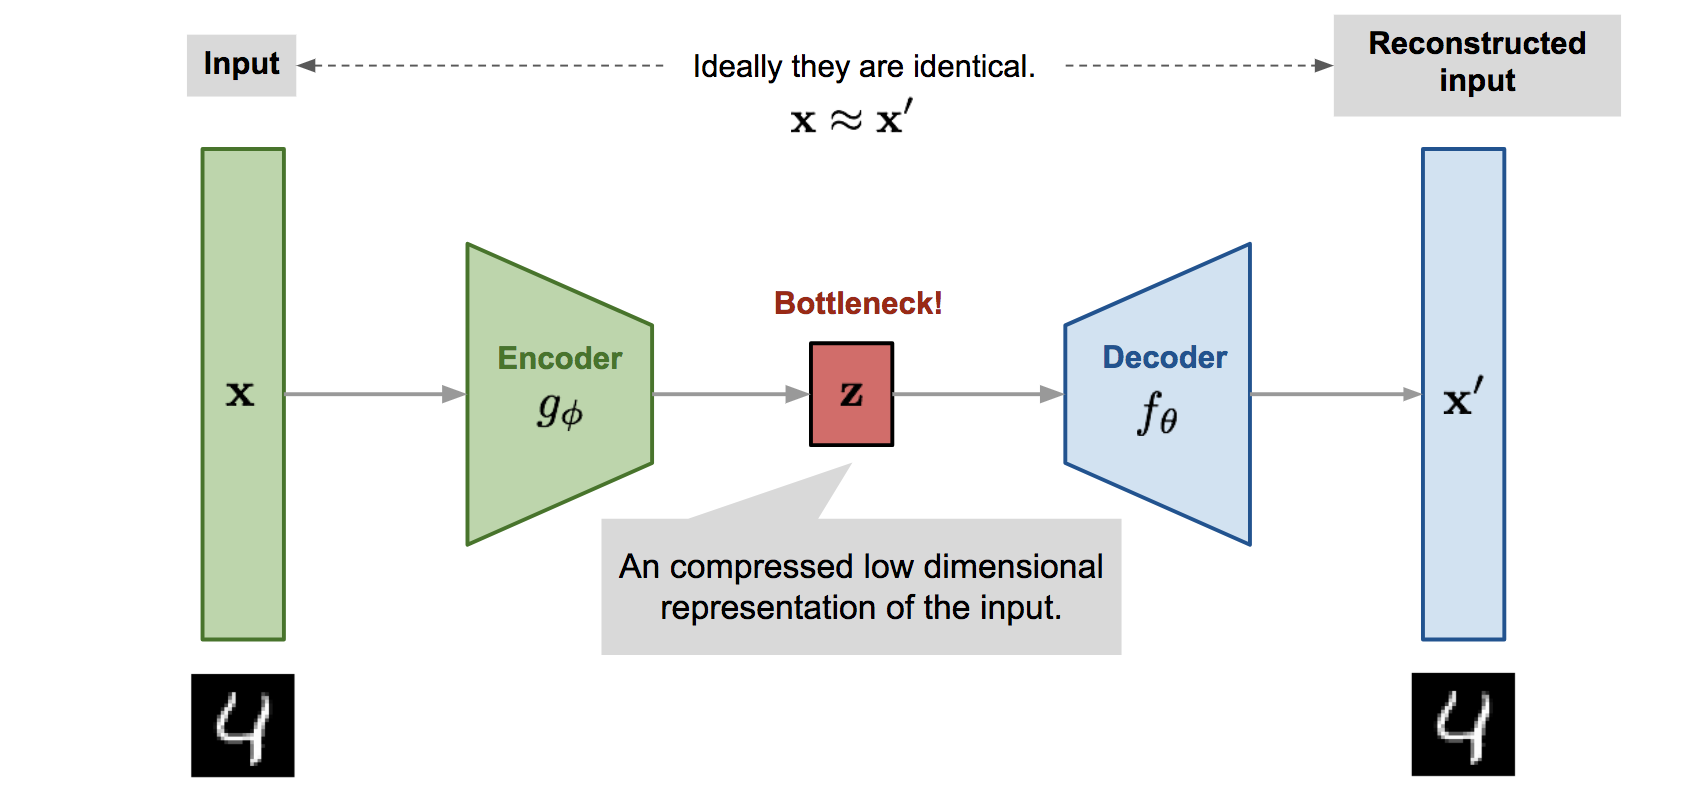
\includegraphics[scale=.55]{../media/autoencoder-architecture.png}
	\caption{Architecture of an autoencoder, consisting of an encoder that compresses the input data into a lower-dimensional latent representation and a decoder that reconstructs the input from this latent space~\cite{Khandelwal:2021}}
	\label{autoencoder}
\end{figure}

Autoencoders are neural networks used primarily for unsupervised learning, particularly in the tasks of dimensionality reduction, feature learning, and anomaly detection. An autoencoder consists of two main components: the encoder and the decoder. The encoder compresses the input data into a latent representation, while the decoder attempts to reconstruct the original data from this compressed representation, as shown in Figure~\ref{autoencoder}.

Mathematically, the \textbf{encoding process} can be represented as:
\begin{equation}
z = g(x; \phi)
\end{equation}
where \( x \) denotes the input data (such as an image or a feature vector), \( g \) is the encoder function that maps \( x \) to the latent representation \( z \), and \( \phi \) represents the parameters (weights and biases) of the encoder network. The latent representation \( z \) captures the essential features of the input in a lower-dimensional space.

The \textbf{decoding process} can be written as:
\begin{equation}
x' = f(z; \theta)
\end{equation}
where \( x' \) is the reconstructed output, \( f \) is the decoder function that maps \( z \) back to the input space, and \( \theta \) are the parameters of the decoder network. The goal is to ensure that the reconstructed output \( x' \) closely matches the original input \( x \).

To measure the quality of the reconstruction, a loss function is employed. Typically, the Mean Squared Error (MSE) is used:
\begin{equation}
L(x, x') = \|x - x'\|^2
\end{equation}
where \( L(x, x') \) represents the loss between the original input \( x \) and the reconstructed output \( x' \). The training process aims to minimize this loss by optimizing the parameters \( \phi \) and \( \theta \), ensuring that the autoencoder can accurately reconstruct the input data from the latent representation.

\chapter{Materials and Methods}
\label{chapter3}
\section{Datasets}
The dataset used in this thesis was collected from \textbf{Balluff Matrix Vision GmbH}, including high-resolution images (1280x960) of Nuts, Candles, Balluff Network Interfaces (BNIs), and Printed Circuit Boards (PCBs). It includes both OK (good) and NOK (not okay, defective) images, captured under two setups: optimal conditions and those with intentional camera-induced variations, such as shadow effects, plexiglass reflections, scattered sunlight, and random object placements. These variations were crucial for simulating real-world challenges, providing the necessary data for generating synthetic images that replicate these conditions. NOK images are utilized solely during the evaluation of the anomaly detector, while OK real images are essential for training models to generate synthetic images.
\subsection{Nuts Dataset}
\label{sec:nuts_dataset}
The Nuts dataset includes both OK and NOK images, captured under different setups: Optimal and Setup with bad influences. The total number of images in each category are presented in Table~\ref{tab:nuts-dataset}.

\begin{table}
    \centering
    \caption{Nuts Dataset Summary}
    \label{tab:nuts-dataset}
    \begin{tabular}{lcc}
        \toprule
        \textbf{Condition} & \textbf{Optimal Setup} & \textbf{Bad Influences} \\ 
        \midrule
        OK Images          & 152                    & 305                     \\ 
        NOK Images         & 48                     & 93                      \\ 
        \bottomrule
    \end{tabular}
\end{table}


\textbf{Optimal Setup:}

The images captured under the optimal setup as shown in Figure~\ref{fig:optimal_setup} were taken with consistent lighting and environmental conditions, ensuring high image quality. This setup provides a clear representation of both OK and NOK Nuts, free from any camera-induced variations.
\begin{figure}
    \centering
    \begin{subfigure}[b]{0.45\textwidth}
        \centering
        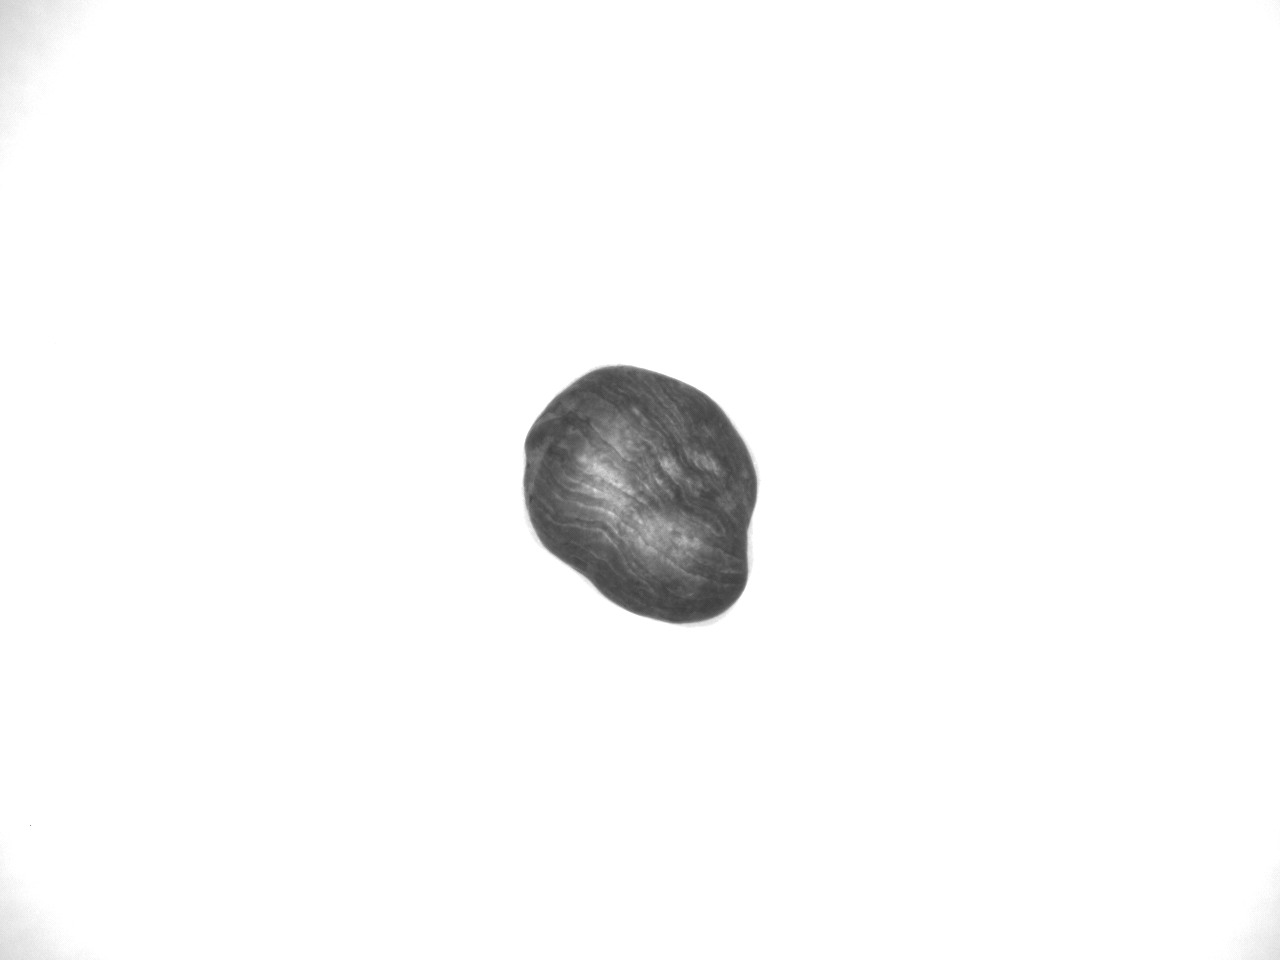
\includegraphics[scale=0.15]{../media/Nuts-Optimal-OK.png}
        \caption{OK nut under optimal setup}
        \label{fig:nut_ok}
    \end{subfigure}
    \hfill
    \begin{subfigure}[b]{0.45\textwidth}
        \centering
        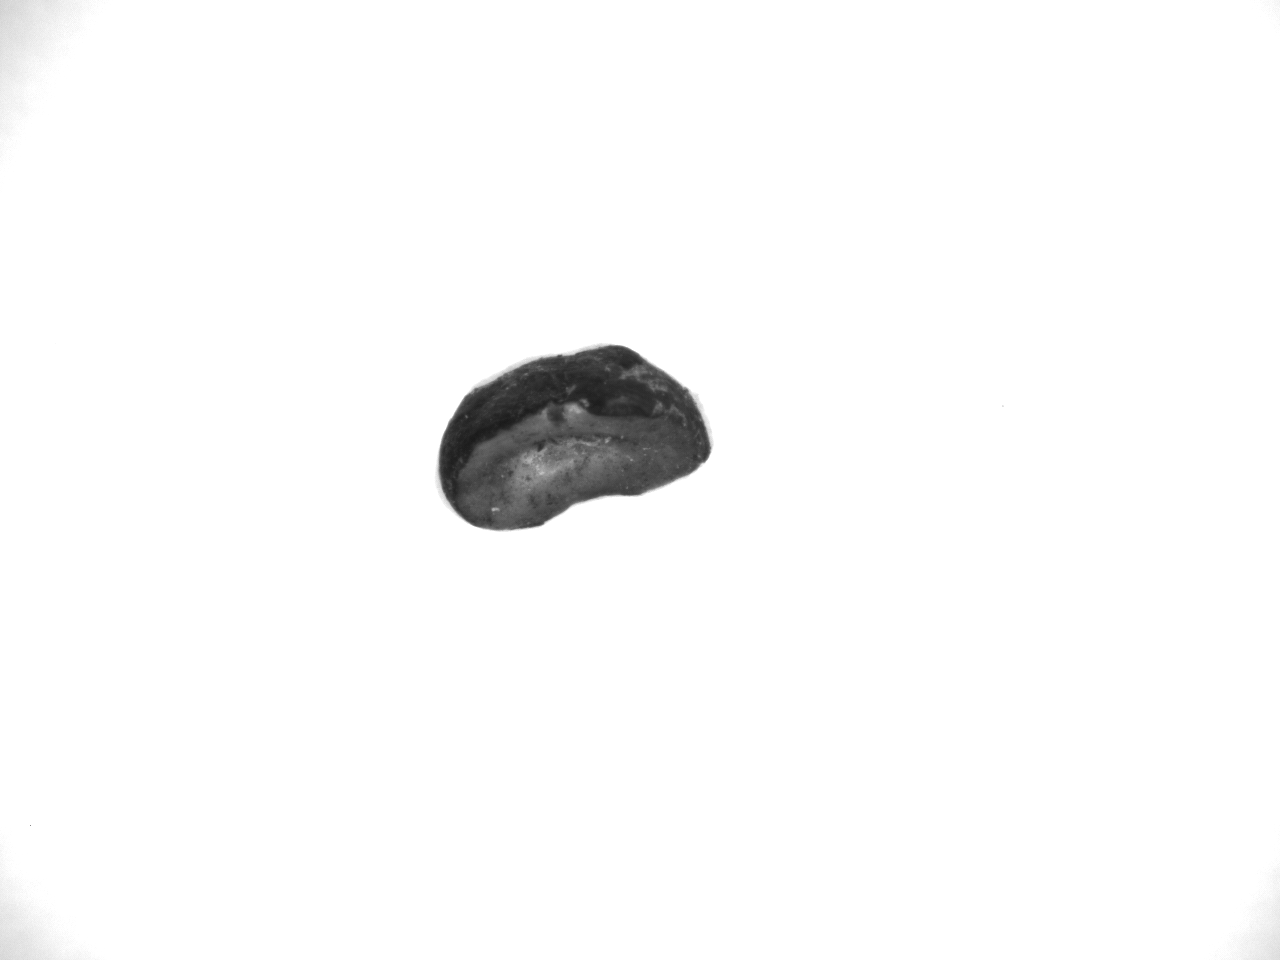
\includegraphics[scale=0.15]{../media/Nuts-optimal-NOK.png}
        \caption{NOK nut under optimal setup}
        \label{fig:nut_nok}
    \end{subfigure}
    \caption{Examples of Nuts captured under optimal setup conditions. (a) OK Nut, exhibiting clear features essential for quality assessment. (b) NOK Nut, showing characteristics that indicate defects. Both images are essential for training and evaluating the anomaly detection system, as they provide a clear baseline of acceptable and unacceptable product qualities.}
    \label{fig:optimal_setup}
\end{figure}

\textbf{Setup with bad influences:}

In this setup, images were captured under conditions that introduced various camera-induced variations, simulating real-world challenges. The following influences were documented:

\begin{enumerate}
	\item \textbf{Shadow Effect:} Shadows occur due to uneven lighting conditions, leading to the formation of dark areas on the Nuts. This influence as shown in Figure~\ref{fig:shadow_effect} can pose a challenge for the anomaly detection system, as the detector might misclassify images with shadows as anomalies if not adequately trained on such variations. The goal is for the anomaly detector to correctly classify genuine NOK images as anomalies while recognizing that OK images affected by shadows should not be labeled as such.

    \begin{figure}
        \centering
        \begin{subfigure}[b]{0.45\textwidth}
            \centering
            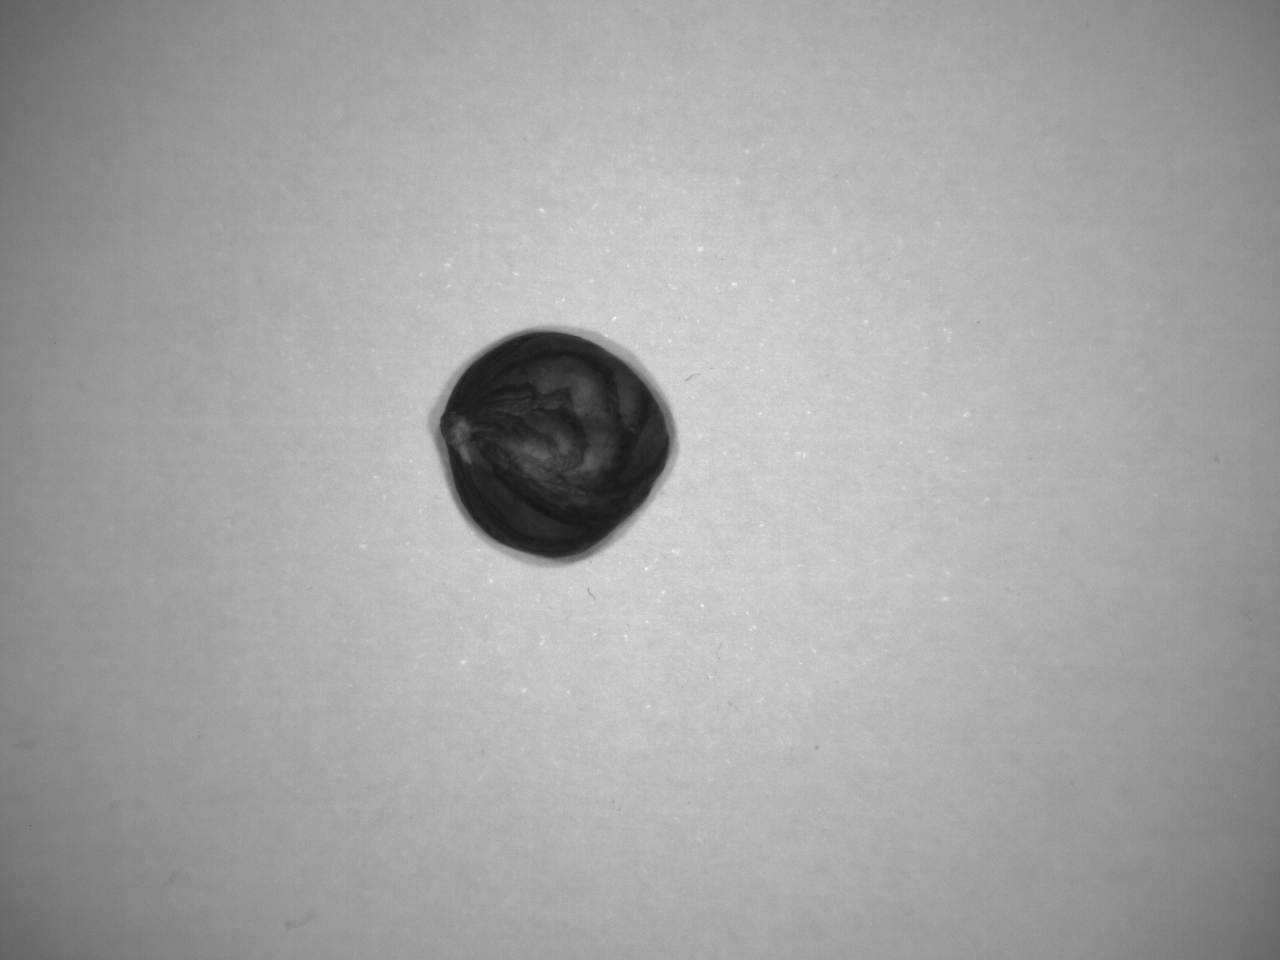
\includegraphics[scale=0.15]{../media/Nuts-influence-shadow-OK.png}
            \caption{OK nut affected by shadow effect}
        \end{subfigure}
        \hfill
        \begin{subfigure}[b]{0.45\textwidth}
            \centering
            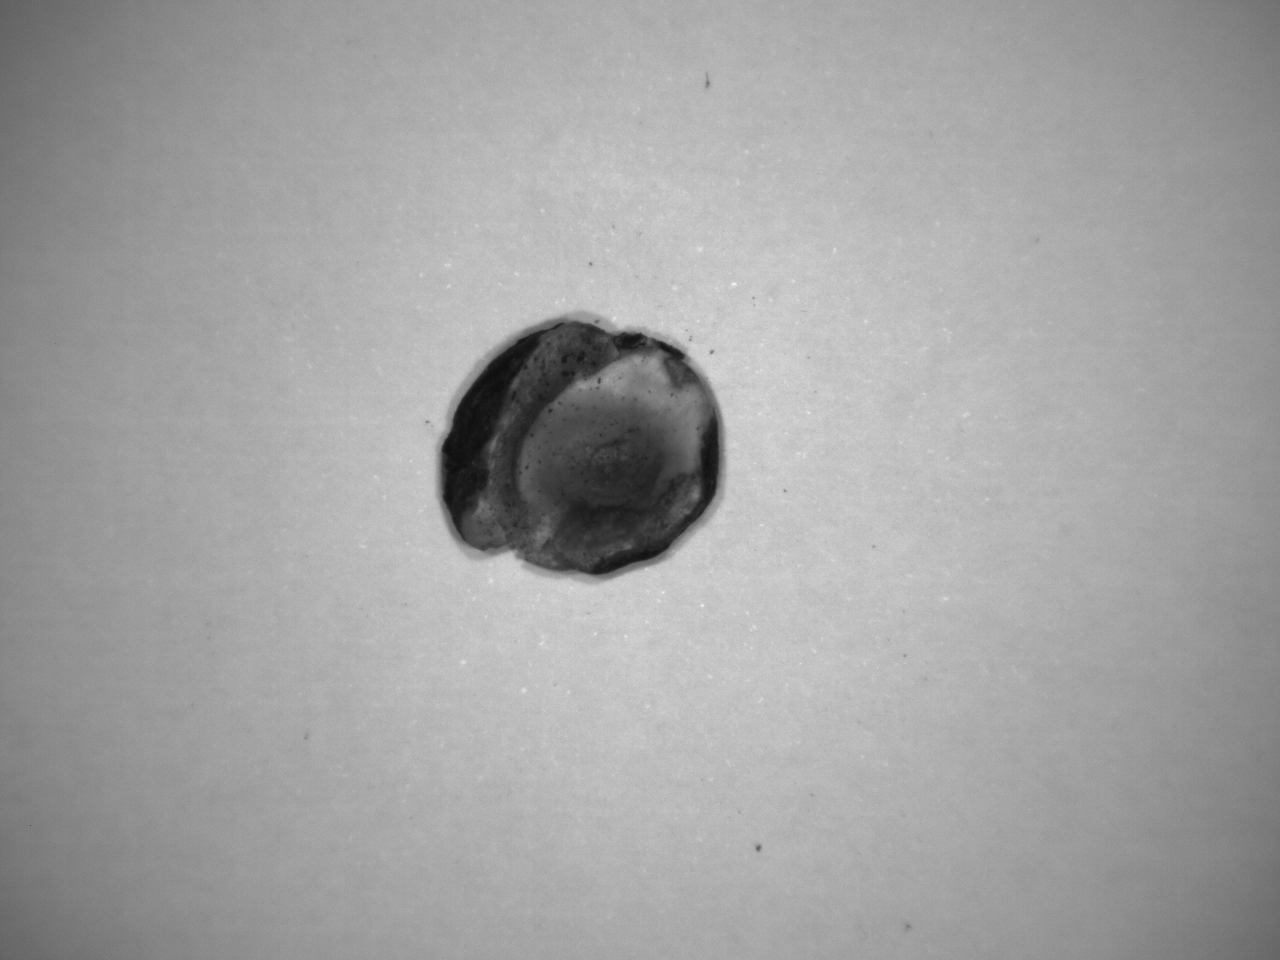
\includegraphics[scale=0.15]{../media/Nuts-influence-shadow-NOK.png}
            \caption{NOK nut affected by shadow effect}
        \end{subfigure}
        \caption{Examples of Nuts affected by shadow effects. (a) OK Nut and (b) NOK Nut.}
        \label{fig:shadow_effect}
    \end{figure}
	\item \textbf{Random Object Placement:} Random object placement refers to the misalignment of the Nuts within the image frame, where the items are not centered or are positioned at varying angles. This can affect the anomaly detection system’s evaluation, as the model might mistakenly identify the irregular positioning as a defect.

	To illustrate this influence, the following images in Figure~\ref{fig:random_object_placement} depict both OK and NOK Nuts affected by random object placement.

	\begin{figure}
		\centering
		\begin{subfigure}[b]{0.45\textwidth}
			\centering
			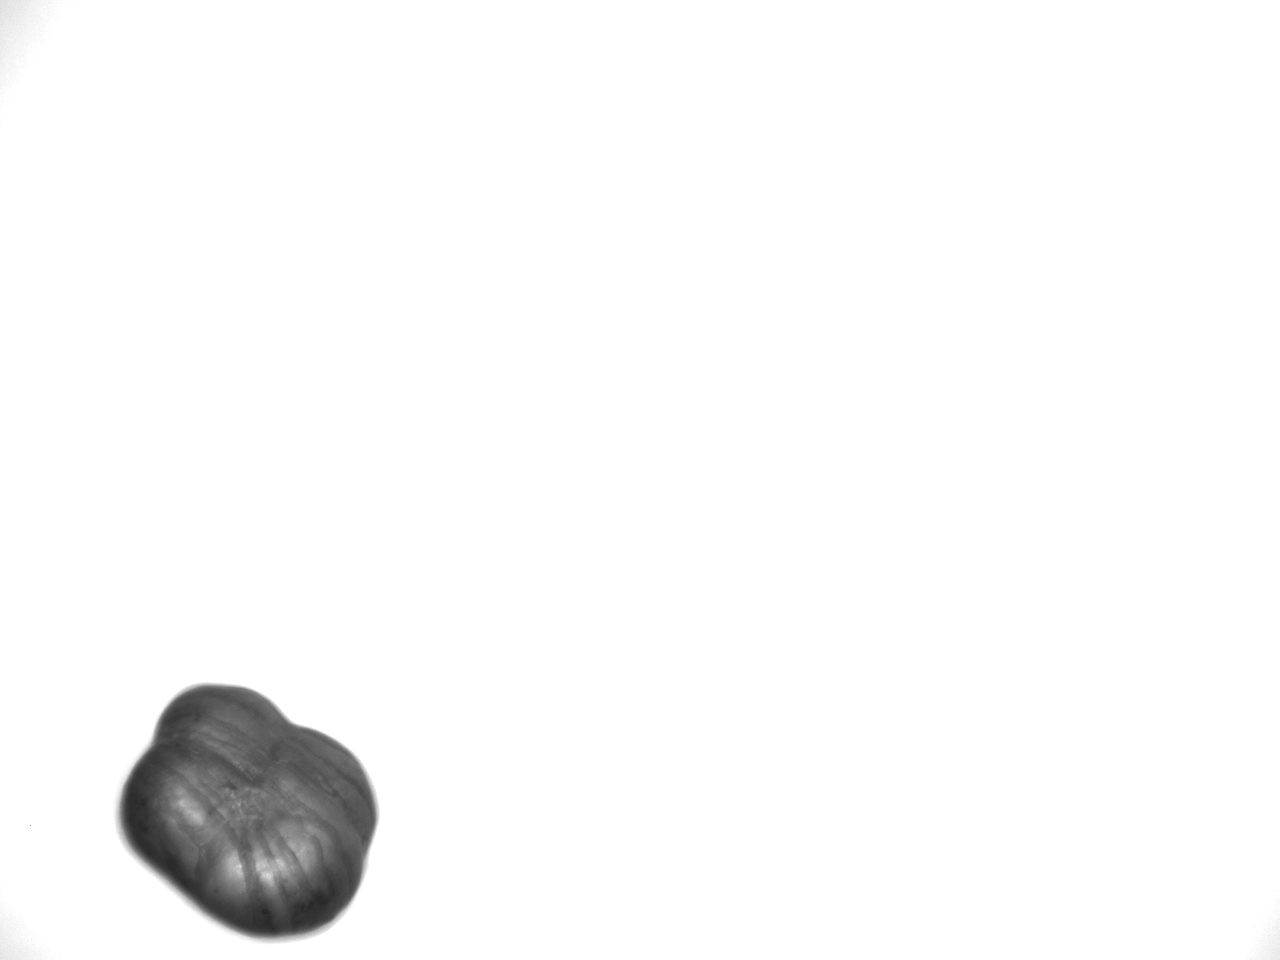
\includegraphics[scale=0.15]{../media/Nuts-influence-random-OK.png}
			\caption{OK nut with random object placement}
		\end{subfigure}
		\hfill
		\begin{subfigure}[b]{0.45\textwidth}
			\centering
			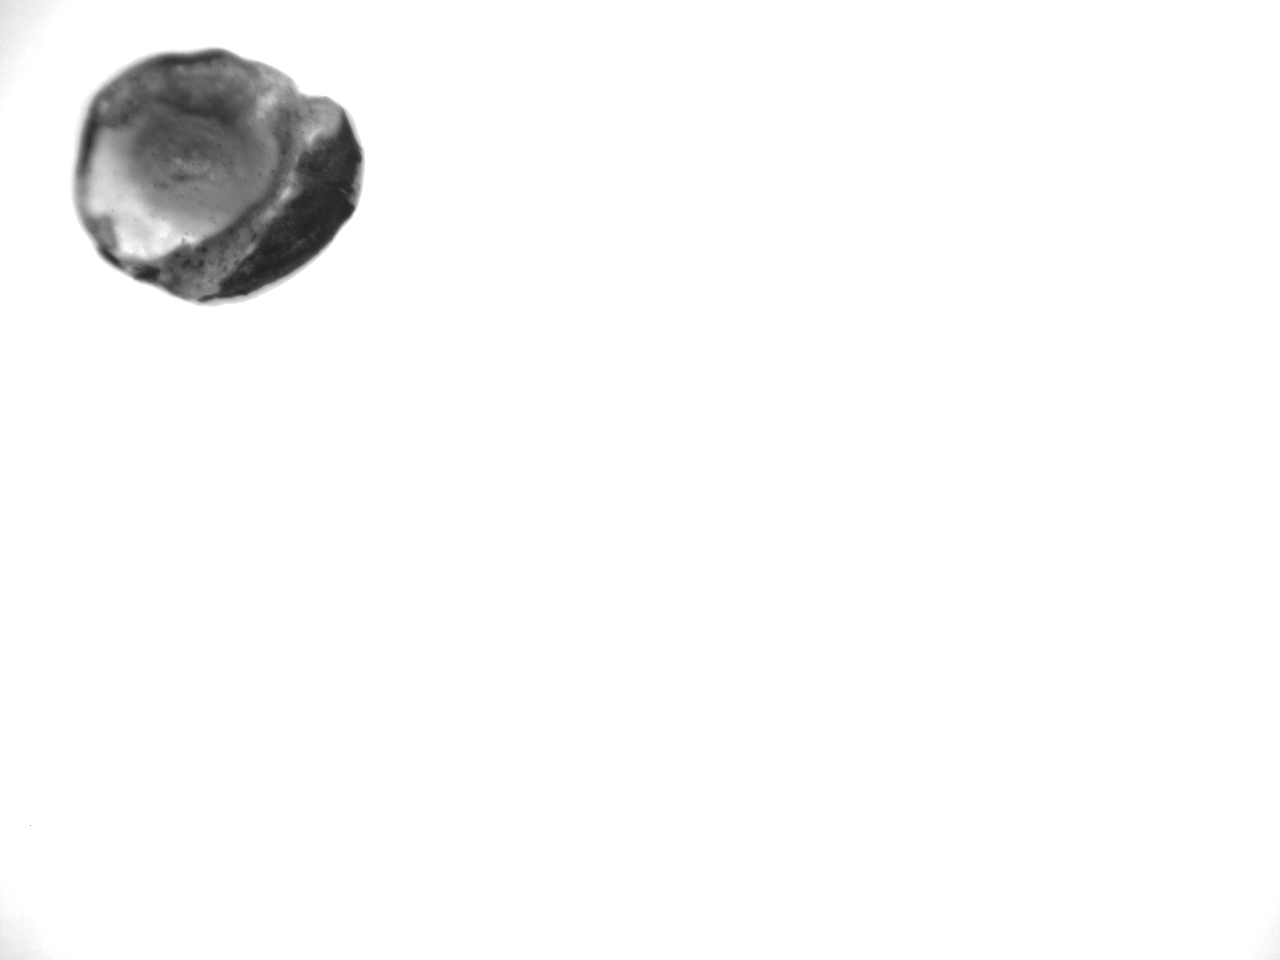
\includegraphics[scale=0.15]{../media/Nuts-influence-random-NOK.png}
			\caption{NOK nut with random object placement}
		\end{subfigure}
		\caption{Examples of Nuts affected by random object placement. (a) OK Nut, and (b) NOK Nut.}
		\label{fig:random_object_placement}
	\end{figure}
	\item \textbf{High Gain Factor:} A high gain factor is applied to increase the sensitivity of the camera sensor, particularly in low-light conditions. While this adjustment can enhance the visibility of the nuts, it also amplifies any inherent noise in the image, resulting in a grainy appearance. This noise can obscure critical features, complicating the evaluation process for the anomaly detection system. If the model is not adequately trained to recognize and differentiate between noise and actual defects, it may mistakenly classify images with high gain as anomalies, leading to inaccurate assessments.
	
	Figure~\ref{fig:high_gain_factor} shows both OK and NOK nuts captured with a high gain factor.
	\begin{figure}
		\centering
		\begin{subfigure}[b]{0.45\textwidth}
			\centering
			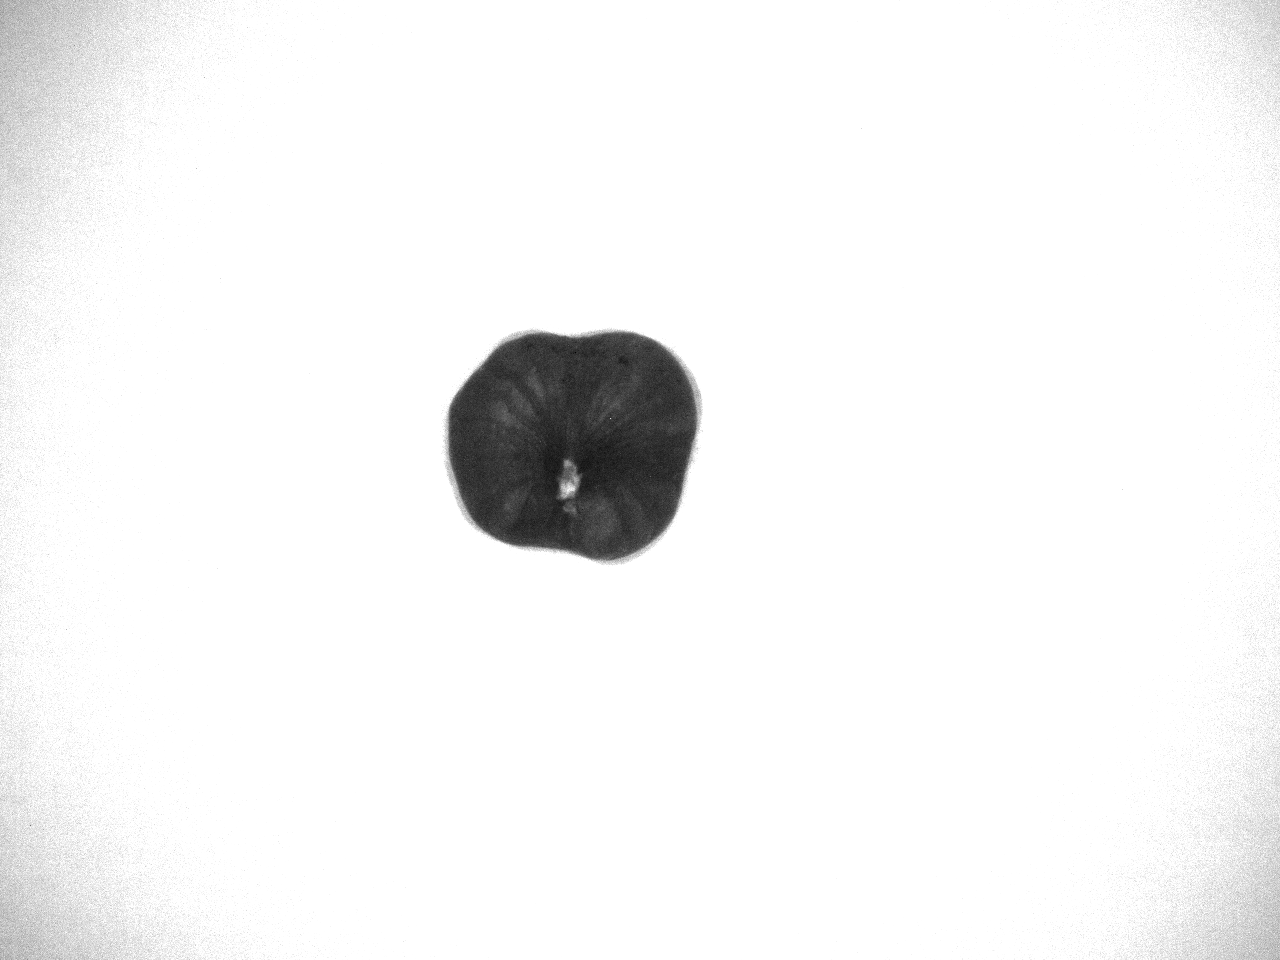
\includegraphics[scale=0.15]{../media/Nuts-influence-highGain-OK.png}
			\caption{OK nut with high gain factor}
		\end{subfigure}
		\hfill
		\begin{subfigure}[b]{0.45\textwidth}
			\centering
			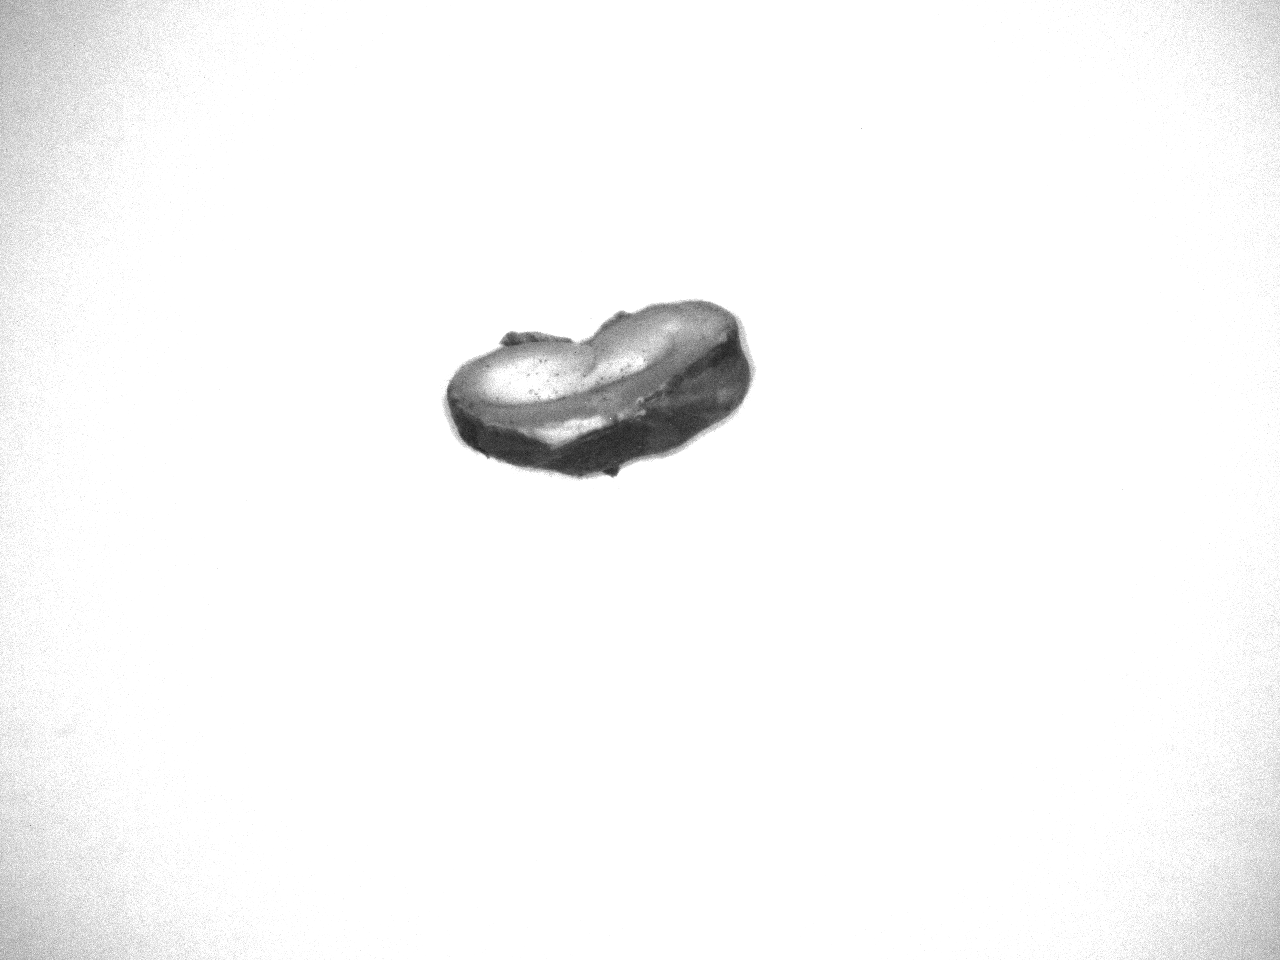
\includegraphics[scale=0.15]{../media/Nuts-influence-highGain-NOK.png}
			\caption{NOK nut with high gain factor}
		\end{subfigure}
		\caption{Examples of nuts affected by a high gain factor. (a) OK Nut, and (b) NOK Nut.}
		\label{fig:high_gain_factor}
	\end{figure}
	\item \textbf{Plexiglas Effect:} The presence of plexiglass can introduce reflections and distortions in the images, affecting the visibility of the nuts. These distortions can complicate the evaluation process for the anomaly detection system, as it may misinterpret the reflections as defects in the product.

	Figure~\ref{fig:plexiglass_effect} showcases examples of both OK and NOK Nuts affected by the plexiglass effect.

	\begin{figure}
		\centering
		\begin{subfigure}[b]{0.45\textwidth}
			\centering
			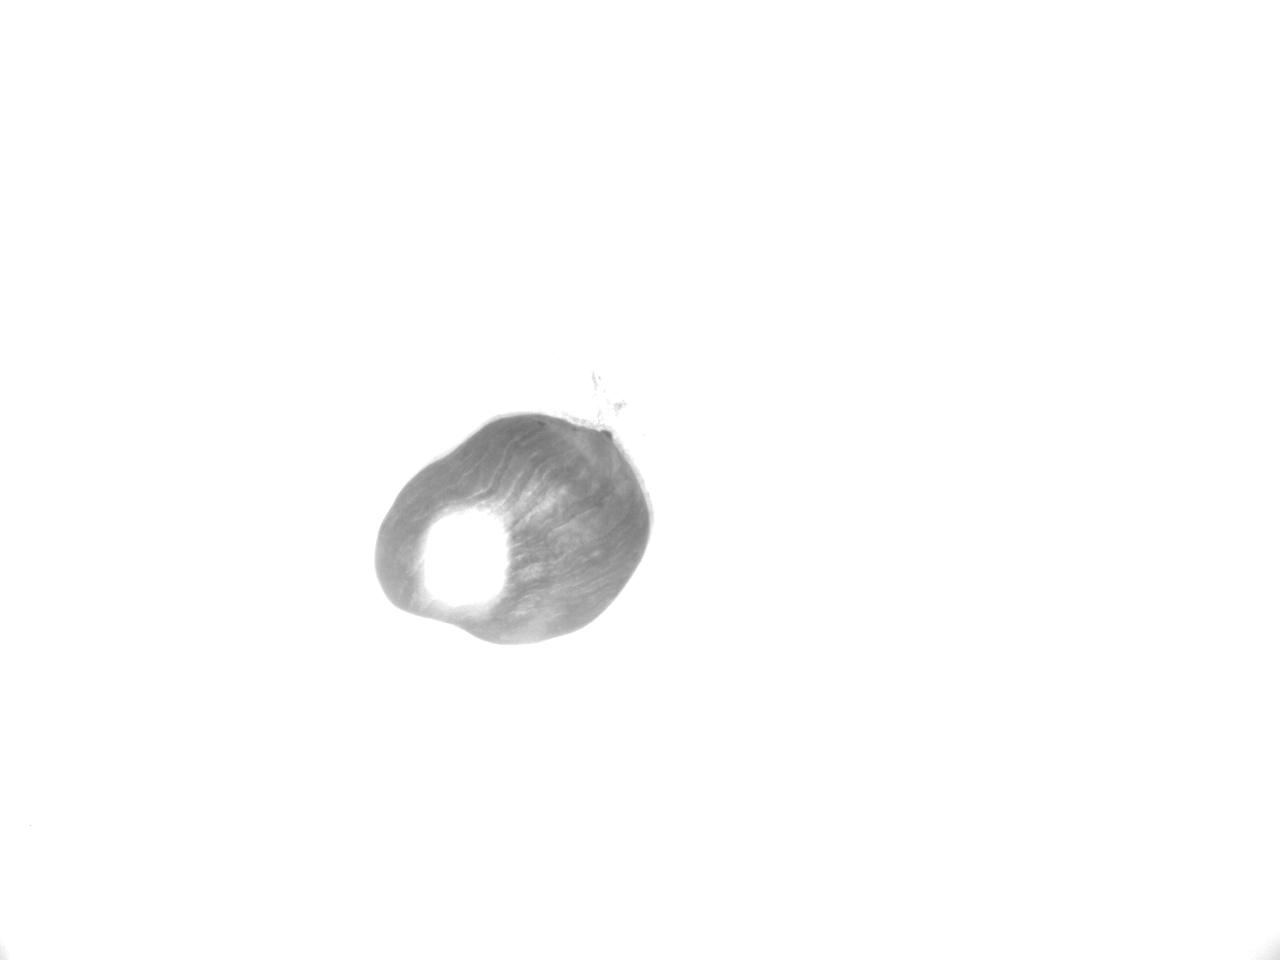
\includegraphics[scale=0.15]{../media/Nuts-influence-plexiglas-OK.png}
			\caption{OK nut affected by plexiglass effect}
		\end{subfigure}
		\hfill
		\begin{subfigure}[b]{0.45\textwidth}
			\centering
			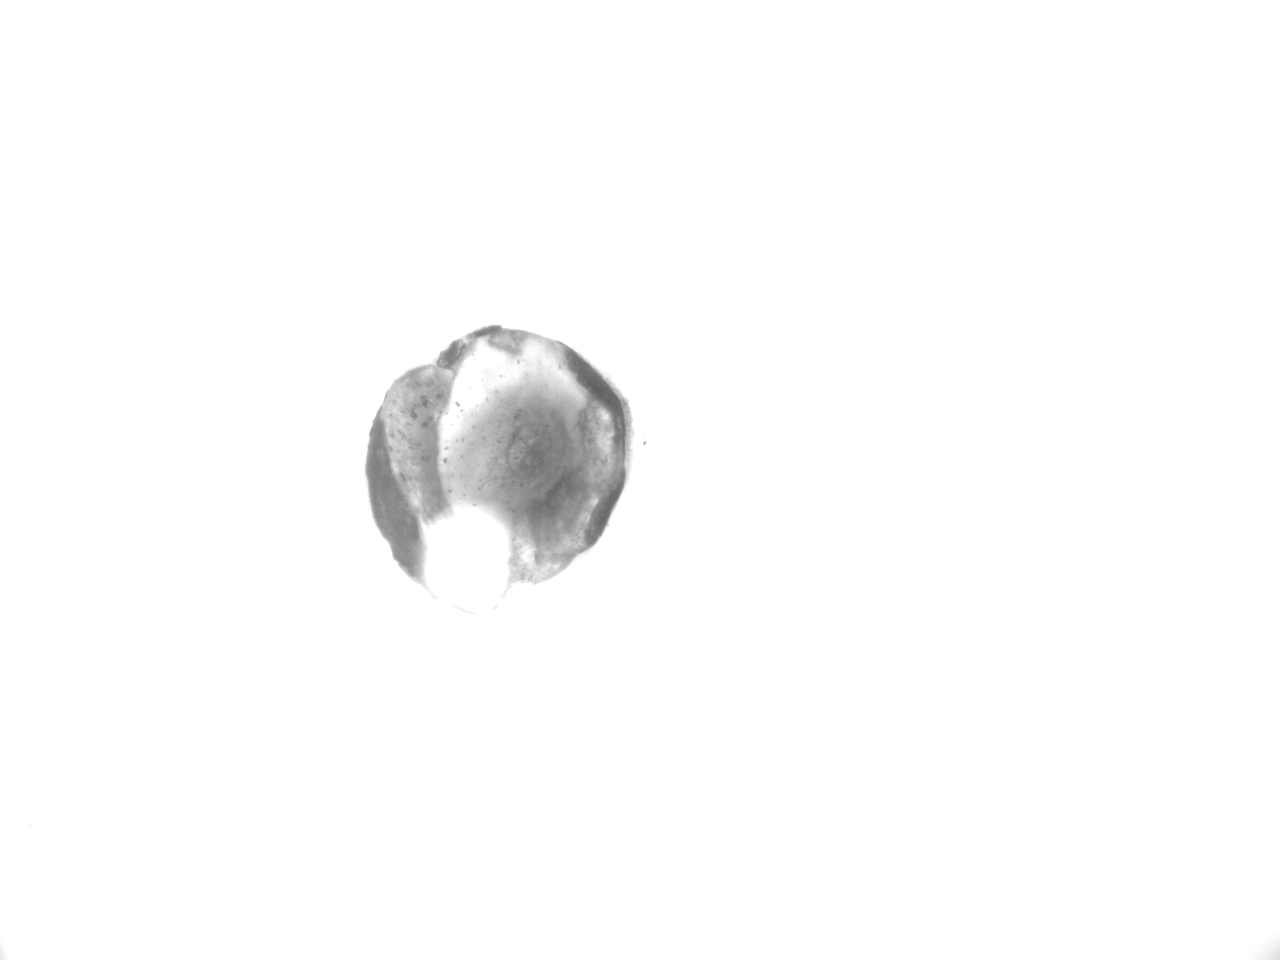
\includegraphics[scale=0.15]{../media/Nuts-influence-plexiglas-NOK.png}
			\caption{NOK nut affected by plexiglass effect}
		\end{subfigure}
		\caption{Examples of Nuts affected by the plexiglass effect. (a) OK Nut, and (b) NOK Nut.}
		\label{fig:plexiglass_effect}
	\end{figure}
\end{enumerate}

\subsection{Candles Dataset}
\label{sec:candles_dataset}
The Candles dataset consists of both OK and NOK images, captured under two different setups: optimal conditions and setups with various camera-induced influences. The details of the dataset are summarized in Table~\ref{tab:candles-dataset}.

\begin{table}
    \centering
    \caption{Candles Dataset Summary}
    \label{tab:candles-dataset}
    \begin{tabular}{lcc}
        \toprule
        \textbf{Condition} & \textbf{Optimal Setup} & \textbf{Bad Influences} \\ 
        \midrule
        OK Images          & 145                    & 134                     \\ 
        NOK Images         & 51                     & 86                      \\ 
        \bottomrule
    \end{tabular}
\end{table}



\textbf{Optimal Setup:}

The images captured under the optimal setup were taken with consistent lighting and environmental conditions, ensuring high image quality. This setup provides a clear representation of both OK and NOK Candles. OK Candles as shown in Figure~\ref{fig:optimal_setup_candles} (a) typically exhibit a round shape, with no dents in the holder or scratches on the candle surface, or absence of the candle or thread in the holder. In contrast, NOK Candles display these irregularities as Figure~\ref{fig:optimal_setup_candles} (b) .

\begin{figure}
    \centering
    \begin{subfigure}[b]{0.45\textwidth}
        \centering
        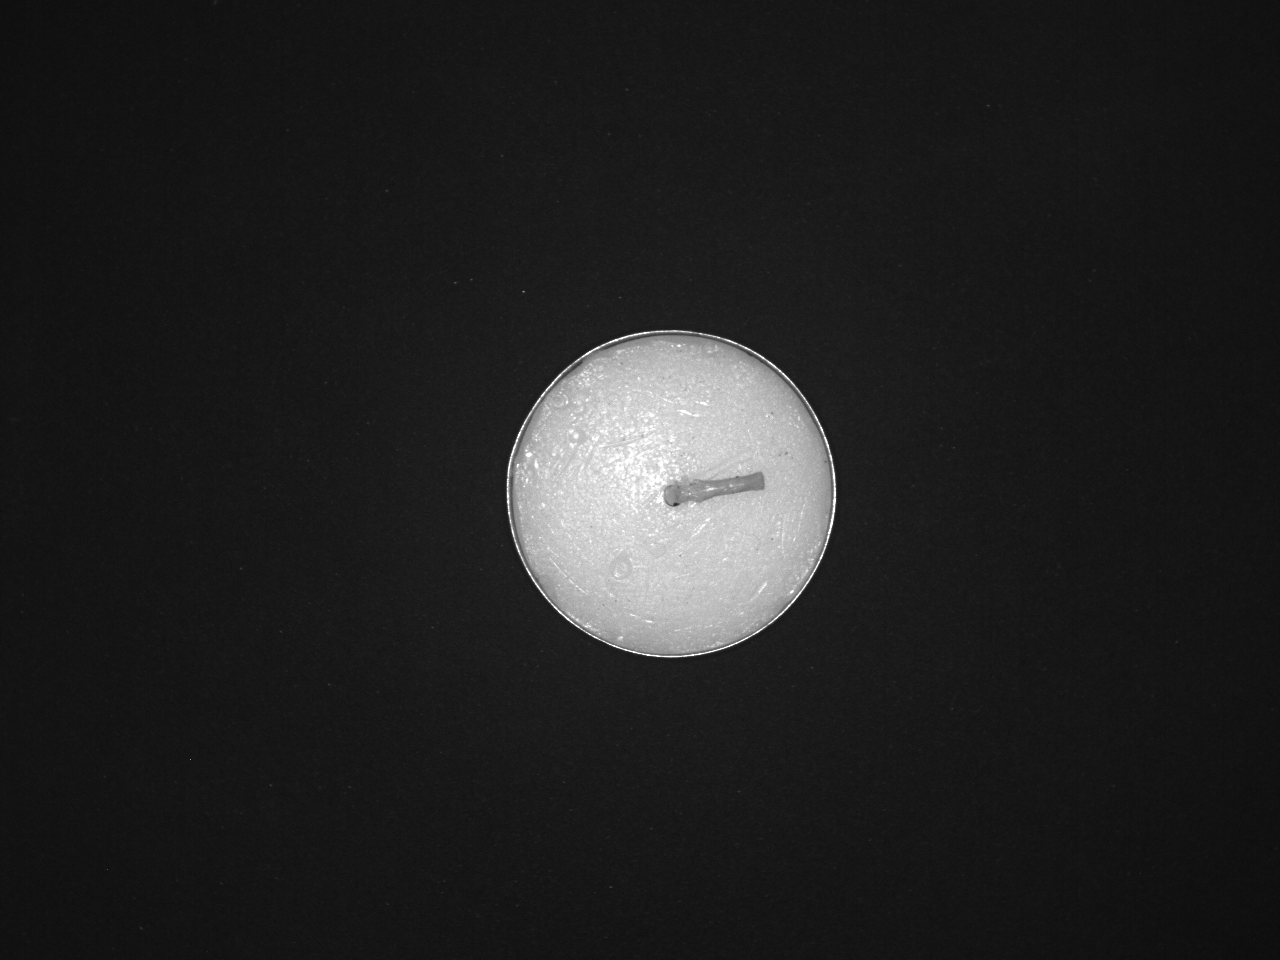
\includegraphics[scale=0.15]{../media/Candles-optimal-OK.png}
        \caption{OK candle under optimal setup}
        \label{fig:candle_ok}
    \end{subfigure}
    \hfill
    \begin{subfigure}[b]{0.45\textwidth}
        \centering
        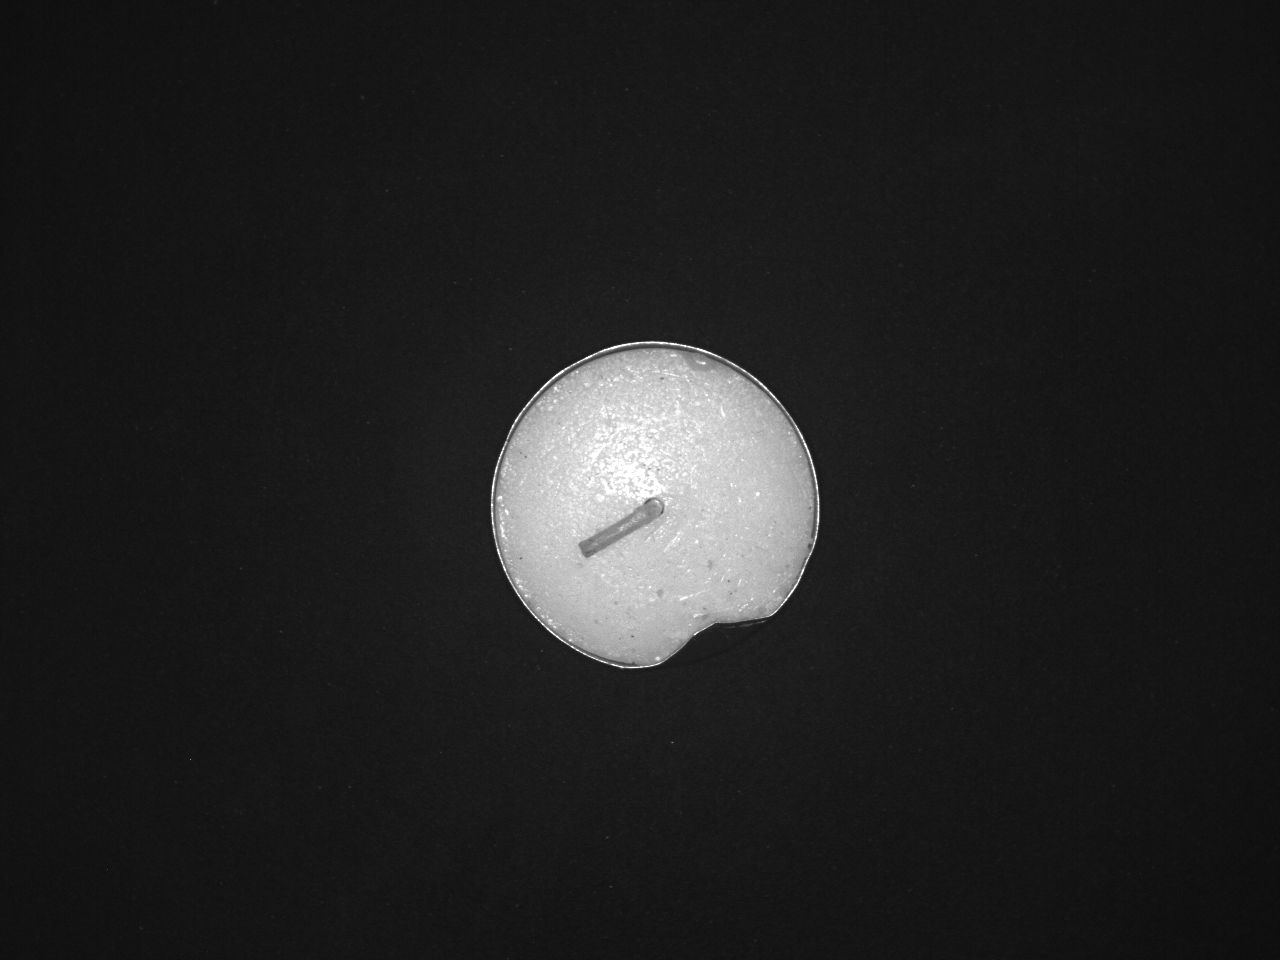
\includegraphics[scale=0.15]{../media/Candles-optimal-NOK.png}
        \caption{NOK candle under optimal setup}
        \label{fig:candle_nok}
    \end{subfigure}
    \caption{Examples of Candles captured under optimal setup conditions. (a) OK Candle, showing smooth and uniform features. (b) NOK Candle, showing defects like dents or scratches.}
    \label{fig:optimal_setup_candles}
\end{figure}

\textbf{Setup with bad influences:}

In this setup, images of Candles were taken under conditions that led to various camera-induced variations, mimicking the challenges encountered in practical scenarios. The following influences were observed:

\begin{enumerate}
    \item \textbf{Scattered Sunlight:} This influence arises when sunlight is diffused or reflected by surrounding objects, leading to uneven illumination on the Candles as shown in Figure~\ref{fig:scattered_sunlight}. The resulting highlights and shadows can obscure important features, potentially complicating the visual evaluation of the Candles quality.

    \begin{figure}
        \centering
        \begin{subfigure}[b]{0.45\textwidth}
            \centering
            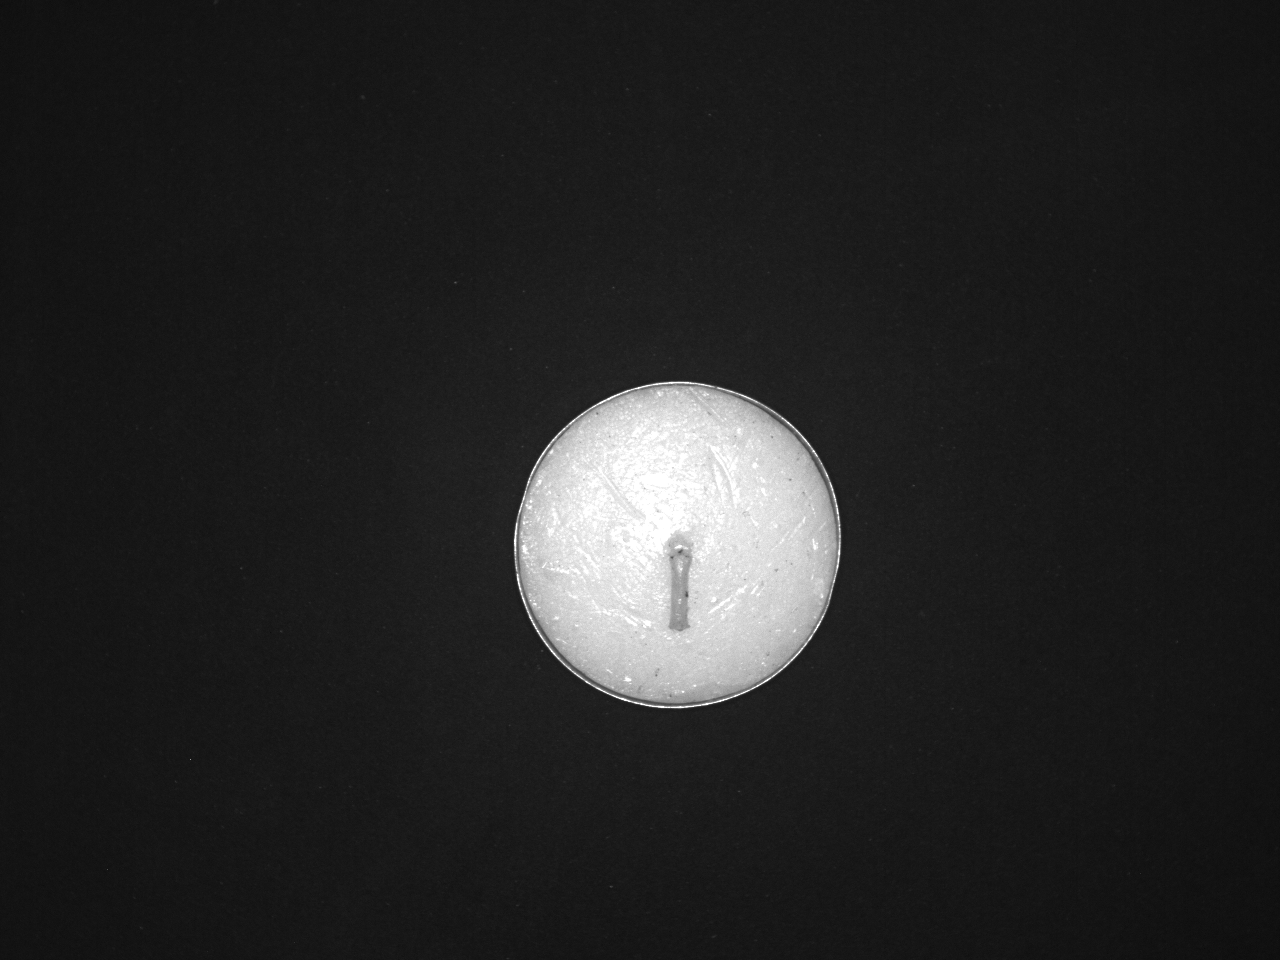
\includegraphics[scale=0.15]{../media/Candles-influence-sunlight-OK.png}
            \caption{OK candle affected by scattered sunlight}
        \end{subfigure}
        \hfill
        \begin{subfigure}[b]{0.45\textwidth}
            \centering
            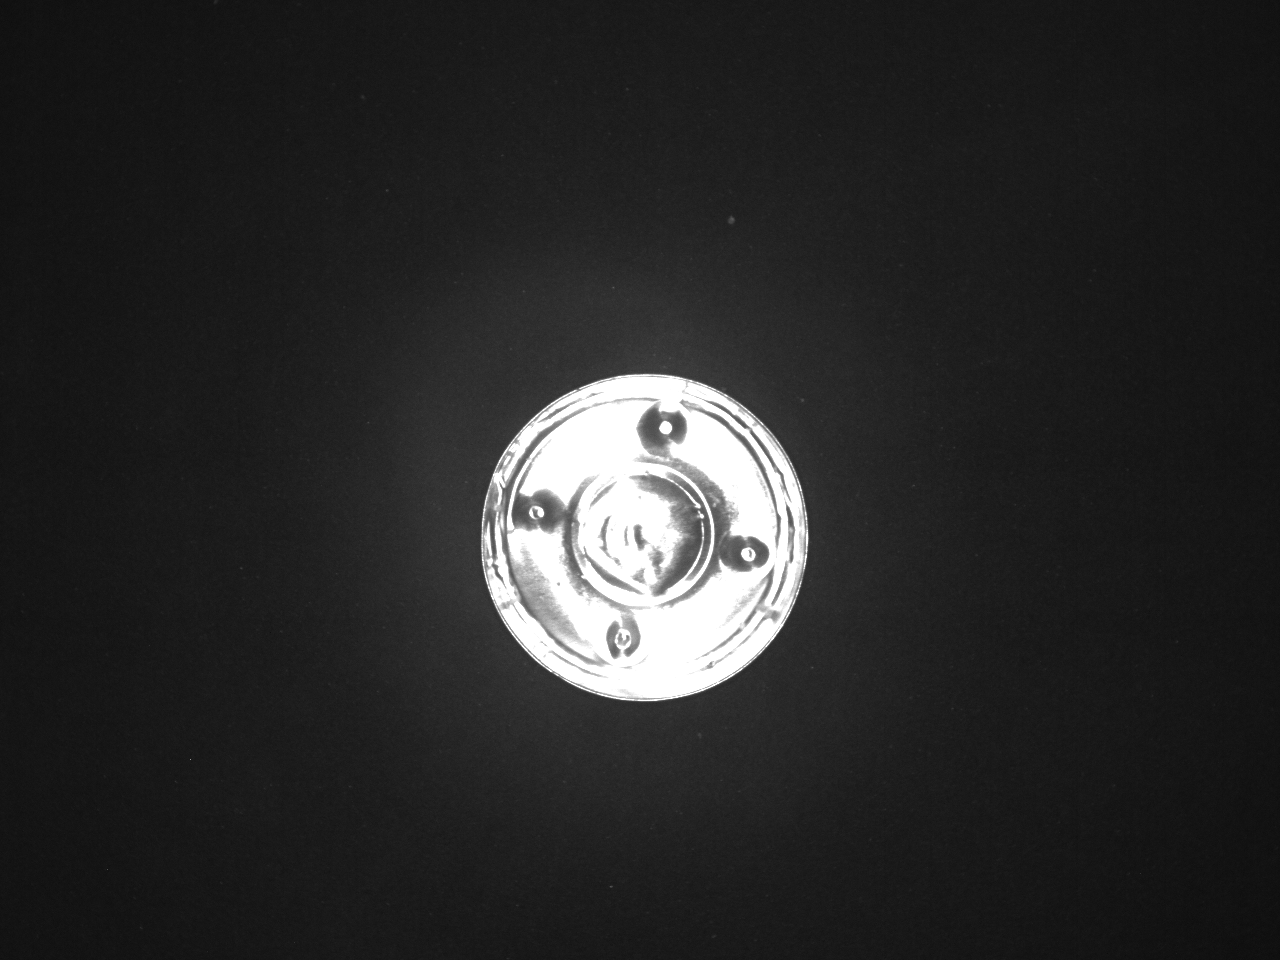
\includegraphics[scale=0.15]{../media/Candles-influence-sunlight-NOK.png}
            \caption{NOK candle affected by scattered sunlight}
        \end{subfigure}
        \caption{Examples of Candles affected by scattered sunlight. (a) OK Candle and (b) NOK Candle, which shows an absence of the candle in the holder}
        \label{fig:scattered_sunlight}
    \end{figure}
	\item \textbf{Random Object Placement:} Random object placement occurs when Candles are not centered within the image frame or are positioned at various angles. This misalignment can lead to confusion in the evaluation process, as the irregular positioning might be interpreted as a defect rather than a mere arrangement issue.
	
	To illustrate this influence, Figure~\ref{fig:random_object_placement_candles} presents examples of both OK and NOK Candles demonstrating random object placement
	
	\begin{figure}
		\centering
		\begin{subfigure}[b]{0.45\textwidth}
			\centering
			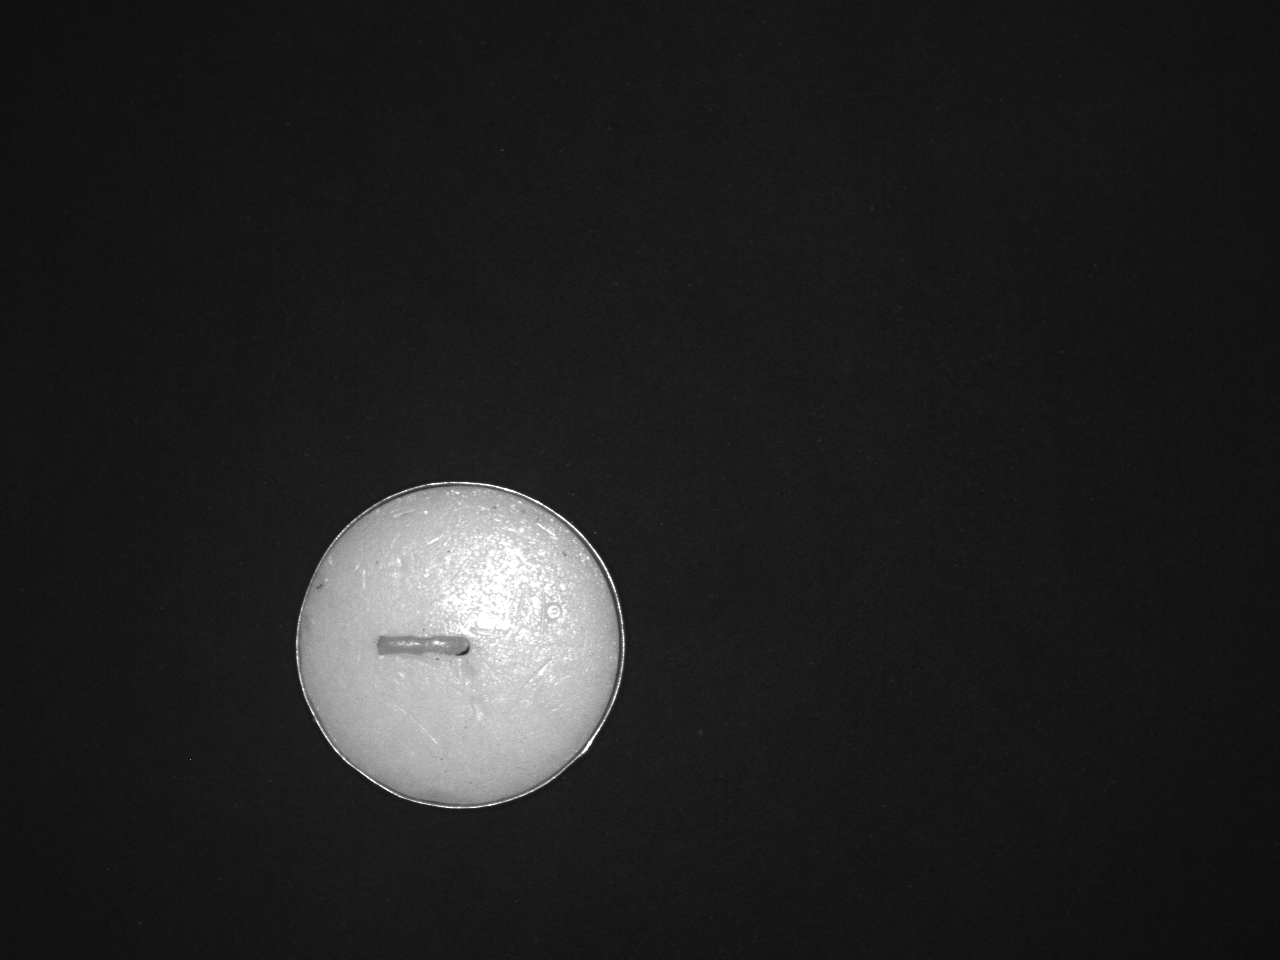
\includegraphics[scale=0.15]{../media/Candles-influence-random-OK.png}
			\caption{OK candle with random object placement}
		\end{subfigure}
		\hfill
		\begin{subfigure}[b]{0.45\textwidth}
			\centering
			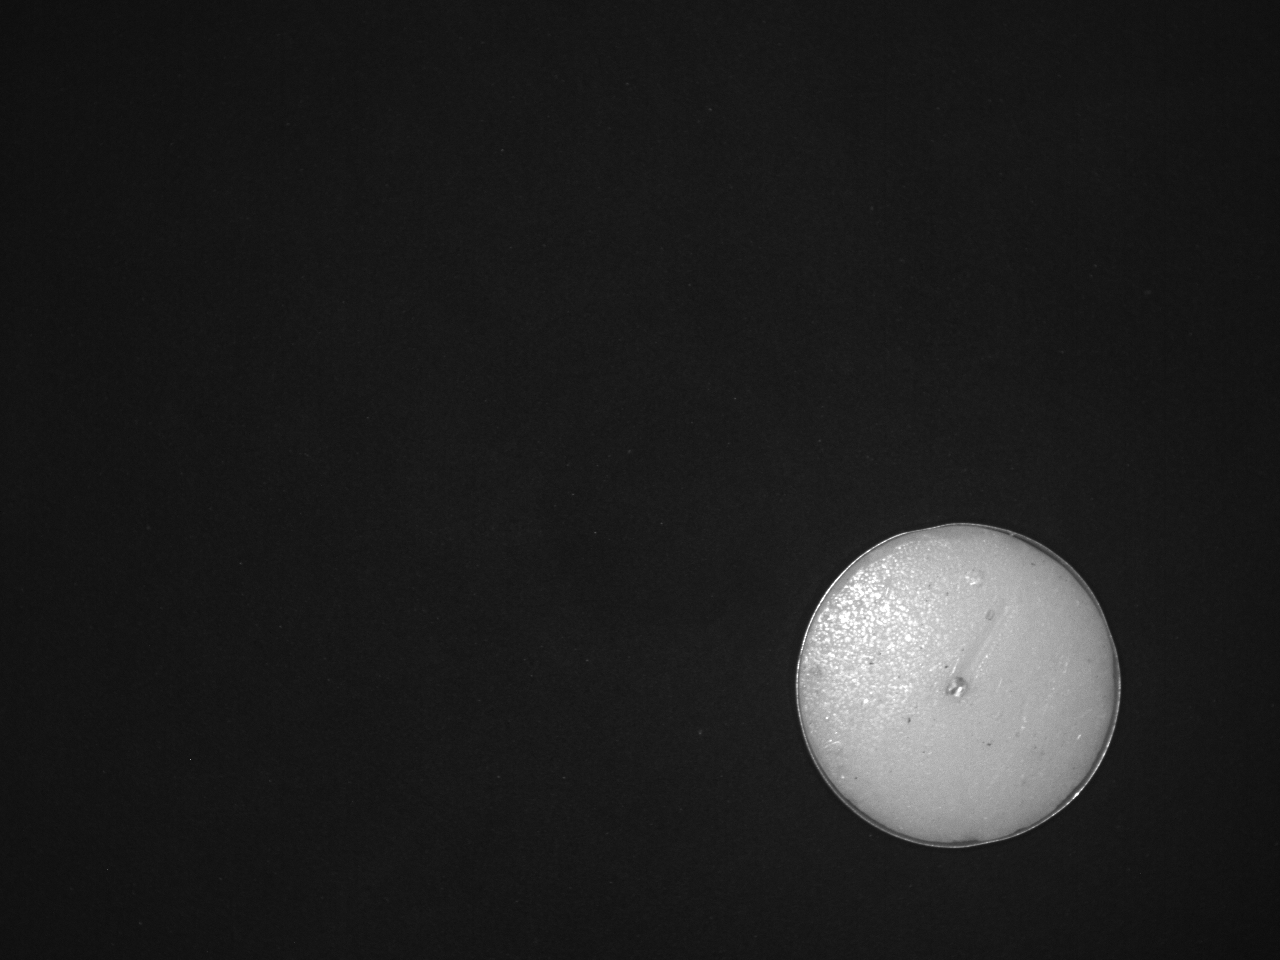
\includegraphics[scale=0.15]{../media/Candles-influence-random-NOK.png}
			\caption{NOK candle with random object placement}
		\end{subfigure}
		\caption{Examples of Candles affected by random object placement. (a) OK Candle and (b) NOK Candle, which shows the absence of the thread on the candle.}
		\label{fig:random_object_placement_candles}
	\end{figure}
	\item \textbf{Camera Elevation (Down):} This setup involves positioning the camera 1 cm down, leading to larger and brighter images of the Candles. 

	To illustrate this influence, the following images in Figure~\ref{fig:camera_elevation_down} depict both OK and NOK Candles affected by this camera elevation.

	\begin{figure}
		\centering
		\begin{subfigure}[b]{0.45\textwidth}
			\centering
			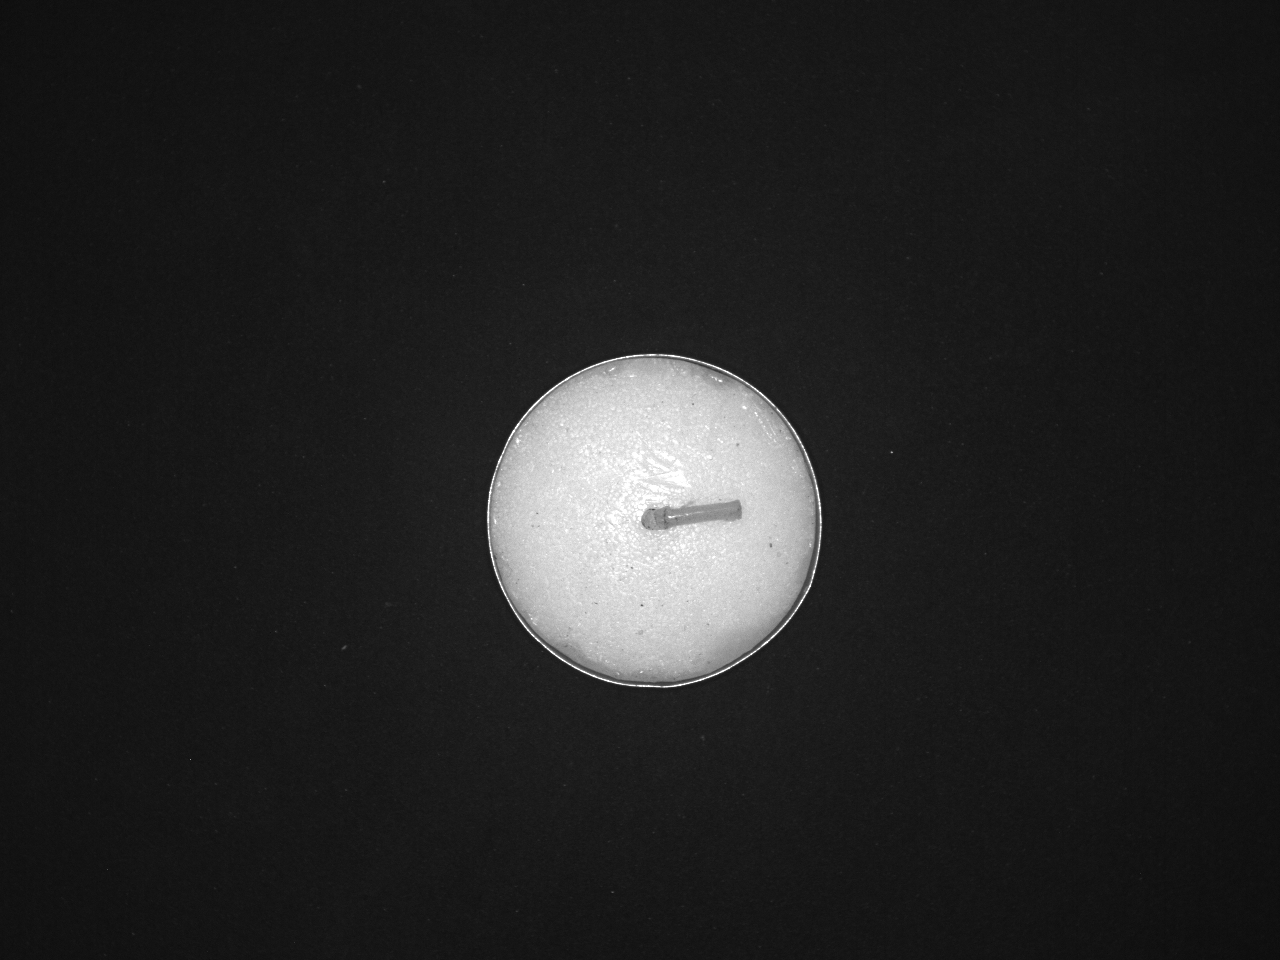
\includegraphics[scale=0.15]{../media/Candles-influence-camera-down-OK.png}
			\caption{OK candle with camera elevation down}
		\end{subfigure}
		\hfill
		\begin{subfigure}[b]{0.45\textwidth}
			\centering
			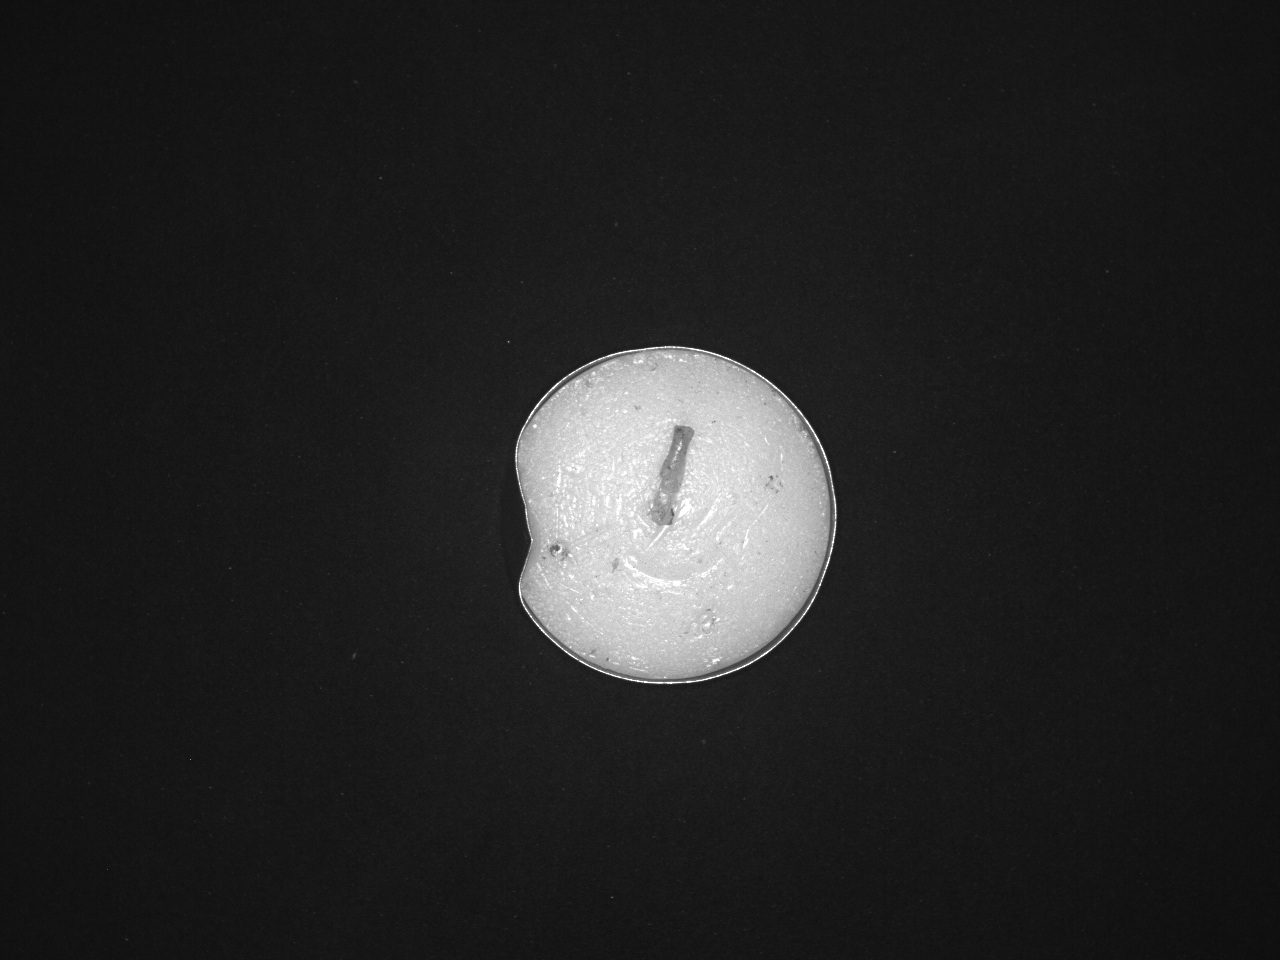
\includegraphics[scale=0.15]{../media/Candles-influence-camera-down-NOK.png}
			\caption{NOK candle with camera elevation down}
		\end{subfigure}
		\caption{Examples of Candles affected by camera elevation down. (a) OK Candle and (b) NOK Candle with dents on the candle holder.}
		\label{fig:camera_elevation_down}
	\end{figure}
	\item \textbf{Camera Elevation (Up):} This setup involves positioning the camera 1 cm up, leading to smaller and darker images of the Candles. 

	To illustrate this influence, the following images in Figure~\ref{fig:camera_elevation_up} depict both OK and NOK Candles affected by this camera elevation.

	\begin{figure}
		\centering
		\begin{subfigure}[b]{0.45\textwidth}
			\centering
			\includegraphics[scale=0.15]{../media/Candles-influence-camera-up-OK.png}
			\caption{OK candle with camera elevation up}
		\end{subfigure}
		\hfill
		\begin{subfigure}[b]{0.45\textwidth}
			\centering
			\includegraphics[scale=0.15]{../media/Candles-influence-camera-up-NOK.png}
			\caption{NOK candle with camera elevation up}
		\end{subfigure}
		\caption{Examples of Candles affected by camera elevation up. (a) OK Candle and (b) NOK Candle.}
		\label{fig:camera_elevation_up}
	\end{figure}
\end{enumerate}
\subsection{BNI Dataset}
BNIs are essential devices in industrial automation, facilitating communication between sensors, actuators, and control systems. The BNI dataset includes both OK and NOK images captured under optimal conditions and various camera-induced influences. The number of images in BNI dataset are summarized in Table~\ref{tab:bni-dataset}.

\begin{table}
    \centering
    \caption{BNI Dataset Summary}
    \label{tab:bni-dataset}
    \begin{tabular}{lcc}
        \toprule
        \textbf{Condition} & \textbf{Optimal Setup} & \textbf{Bad Influences} \\ 
        \midrule
        OK Images          & 44                     & 73                      \\ 
        NOK Images         & 24                     & 48                      \\ 
        \bottomrule
    \end{tabular}
\end{table}


\textbf{Optimal Setup:}

Images taken in the optimal setup featured uniform lighting and controlled environmental conditions, resulting in high-quality visuals as shown in Figure~\ref{fig:optimal_setup_bnis}. OK images display BNIs in good condition, with intact labels and defect-free surfaces, providing a clear representation of expected quality. Conversely, NOK images may lack complete labeling or exhibit irregularities, including instances where epoxy resin has solidified on the BNI surface due to leaks during the potting process.
\begin{figure}
    \centering
    \begin{subfigure}[b]{0.45\textwidth}
        \centering
        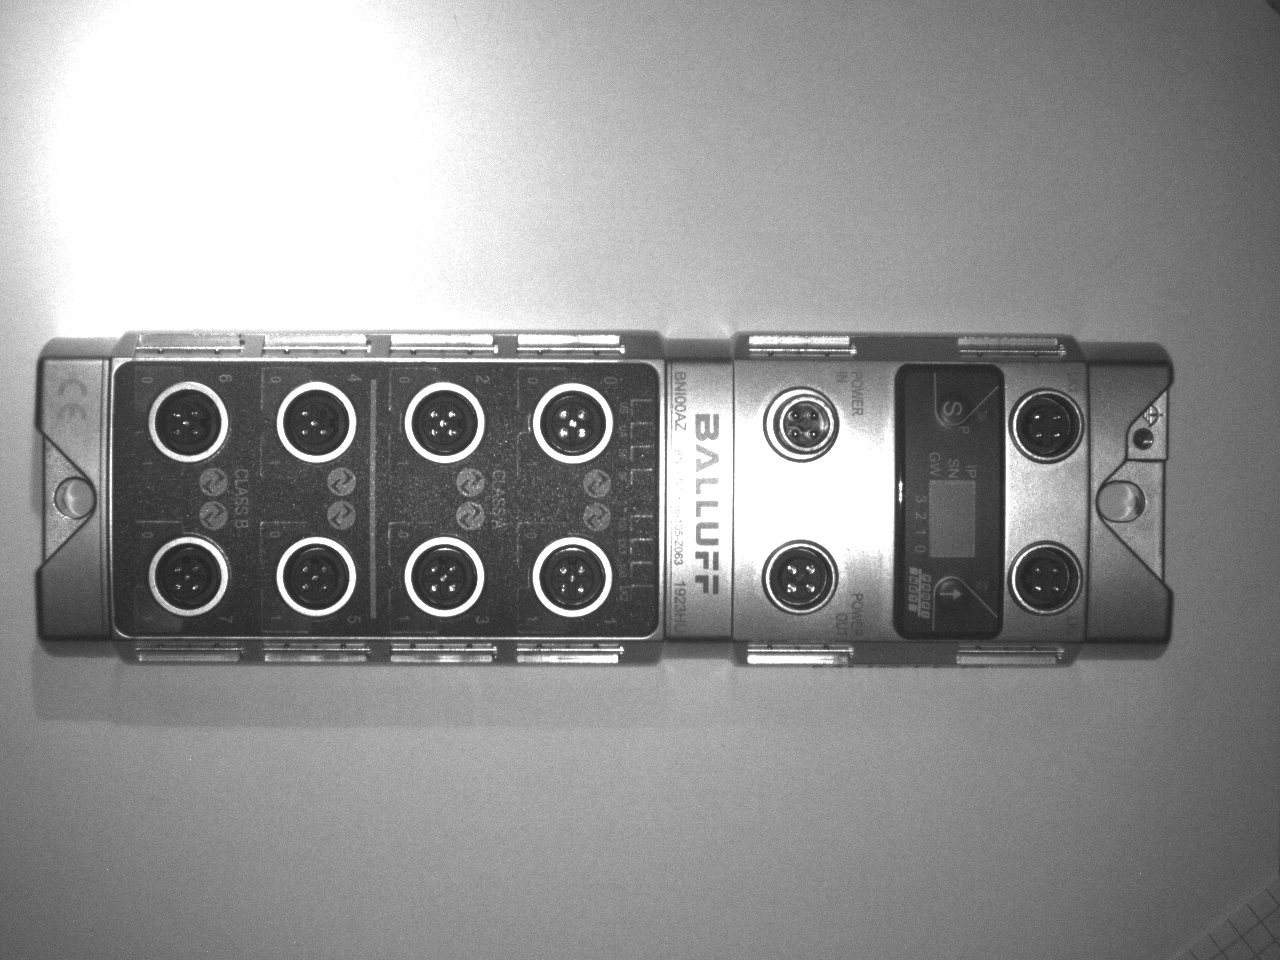
\includegraphics[scale=0.15]{../media/BNI-optimal-OK.png}
        \caption{OK BNI under optimal setup}
        \label{fig:bni_ok}
    \end{subfigure}
    \hfill
    \begin{subfigure}[b]{0.45\textwidth}
        \centering
        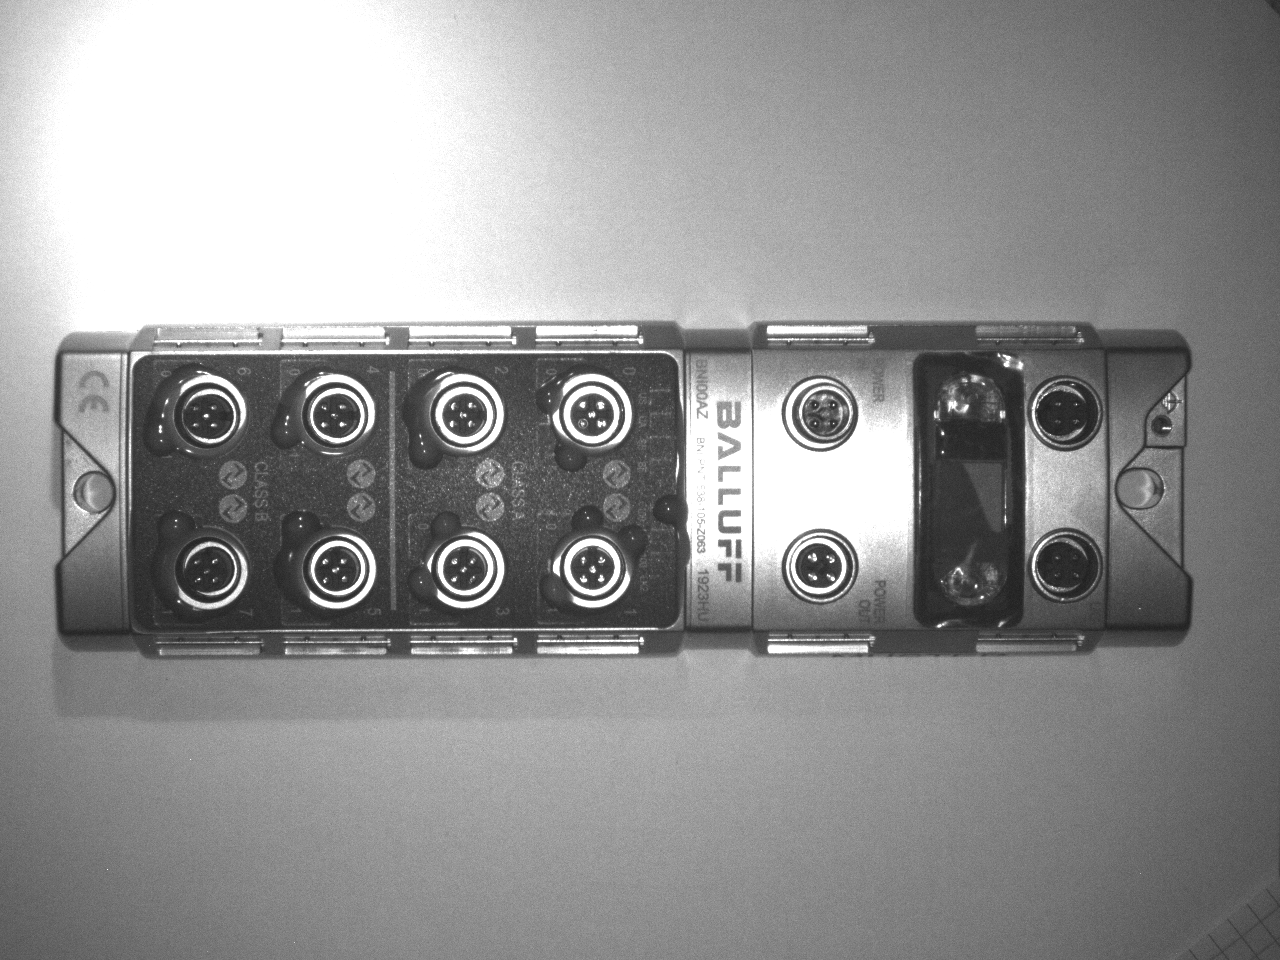
\includegraphics[scale=0.15]{../media/BNI-optimal-NOK.png}
        \caption{NOK BNI under optimal setup}
        \label{fig:bni_nok}
    \end{subfigure}
    \caption{Examples of BNIs captured under optimal setup conditions. (a) OK BNI, displaying intact labels and no surface defects. (b) NOK BNI, showing solidified epoxy resin on the surface.}
    \label{fig:optimal_setup_bnis}
\end{figure}

\textbf{Setup with bad influences:}

In this setup, images of BNIs were taken under conditions that introduced several camera-related distortions, replicating potential challenges in practical industrial settings. The observed influences were as follows:
\begin{enumerate}
    \item \textbf{Inclination (Left):} In this setup, the BNI device was inclined to the left, altering its orientation in the image frame. This shift in perspective can distort the appearance of labels and surfaces, complicating defect detection. 
    
	The impact of left inclination is shown in Figure~\ref{fig:inclination_left}, where both OK and NOK BNIs are depicted with this orientation shift.
    \begin{figure}
        \centering
        \begin{subfigure}[b]{0.45\textwidth}
            \centering
            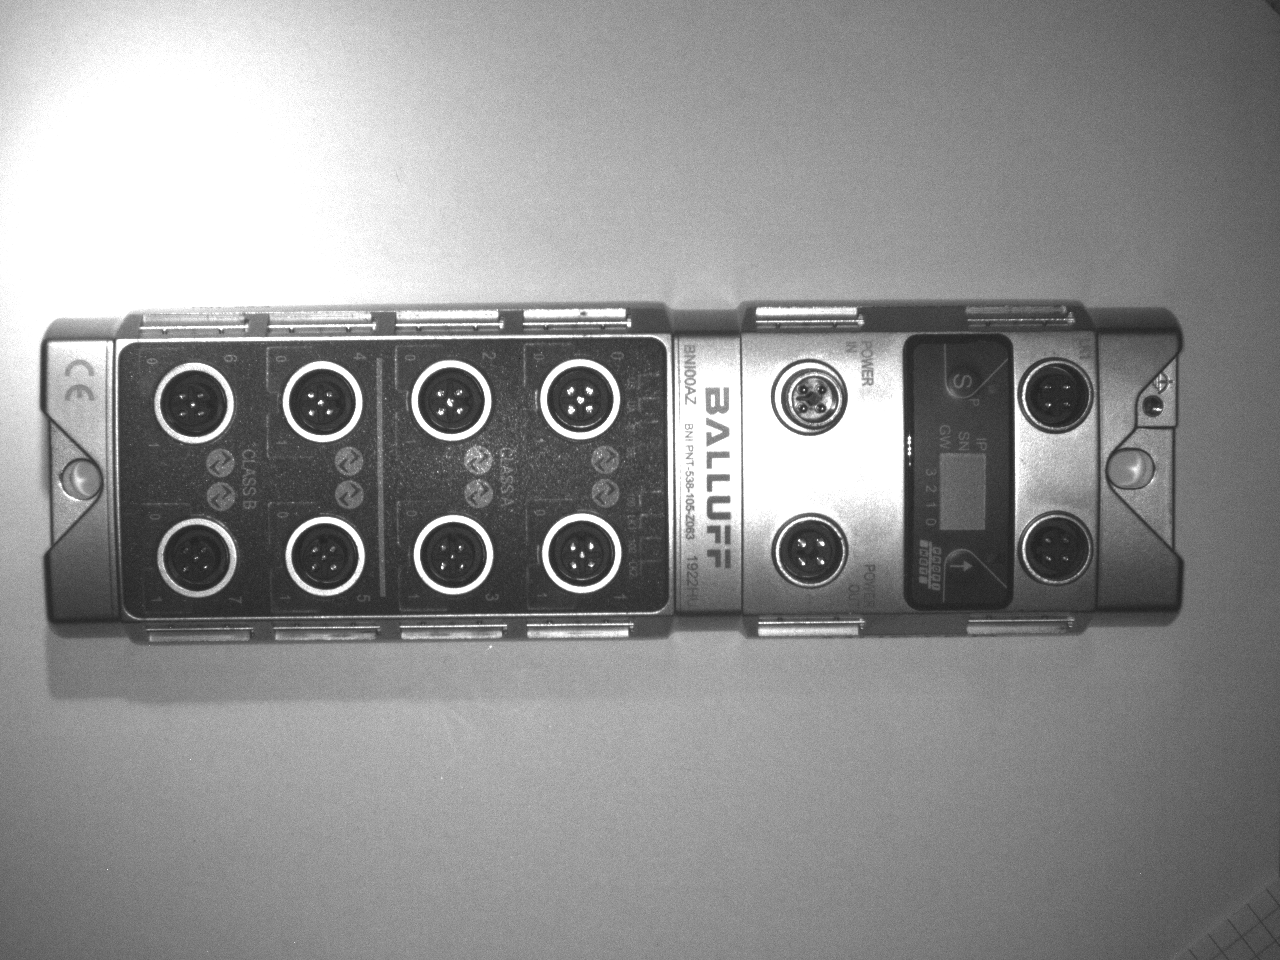
\includegraphics[scale=0.15]{../media/BNI-influence-left-OK.png}
            \caption{OK BNI with left inclination}
        \end{subfigure}
        \hfill
        \begin{subfigure}[b]{0.45\textwidth}
            \centering
            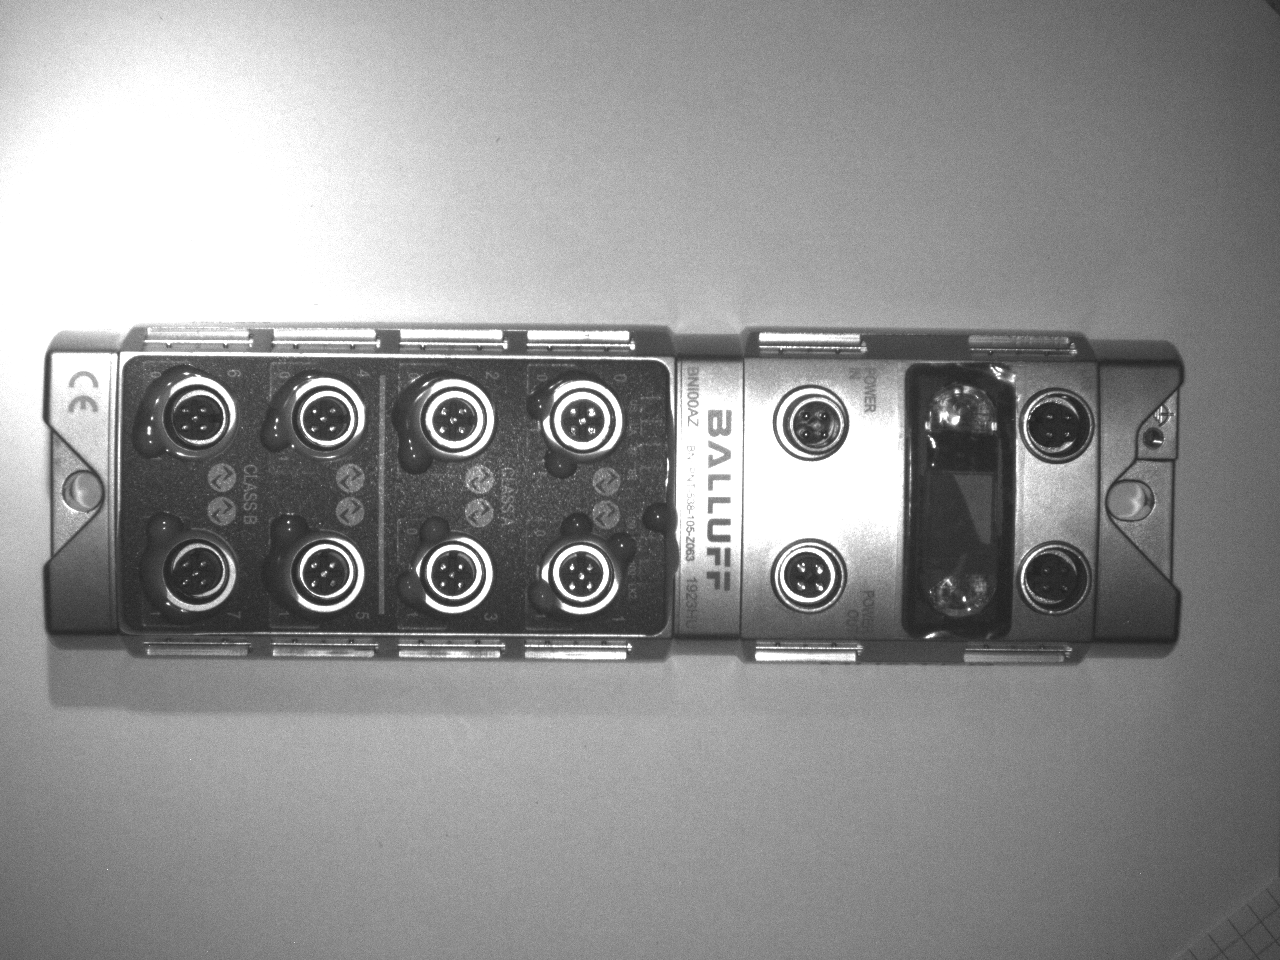
\includegraphics[scale=0.15]{../media/BNI-influence-left-NOK.png}
            \caption{NOK BNI with left inclination}
        \end{subfigure}
        \caption{Examples of BNIs affected by left inclination. (a) OK BNI and (b) NOK BNI with solidified epoxy resin on the surface.}
        \label{fig:inclination_left}
    \end{figure}

    \item \textbf{Inclination (Right):} Similarly, the BNI device was inclined to the right, resulting in a different angle of distortion. This tilt can affect how lighting interacts with the surface, potentially hiding defects or causing glare.
    
	Figure~\ref{fig:inclination_right} presents examples of BNIs subjected to right inclination, illustrating both OK and NOK instances affected by this tilt
    \begin{figure}
        \centering
        \begin{subfigure}[b]{0.45\textwidth}
            \centering
            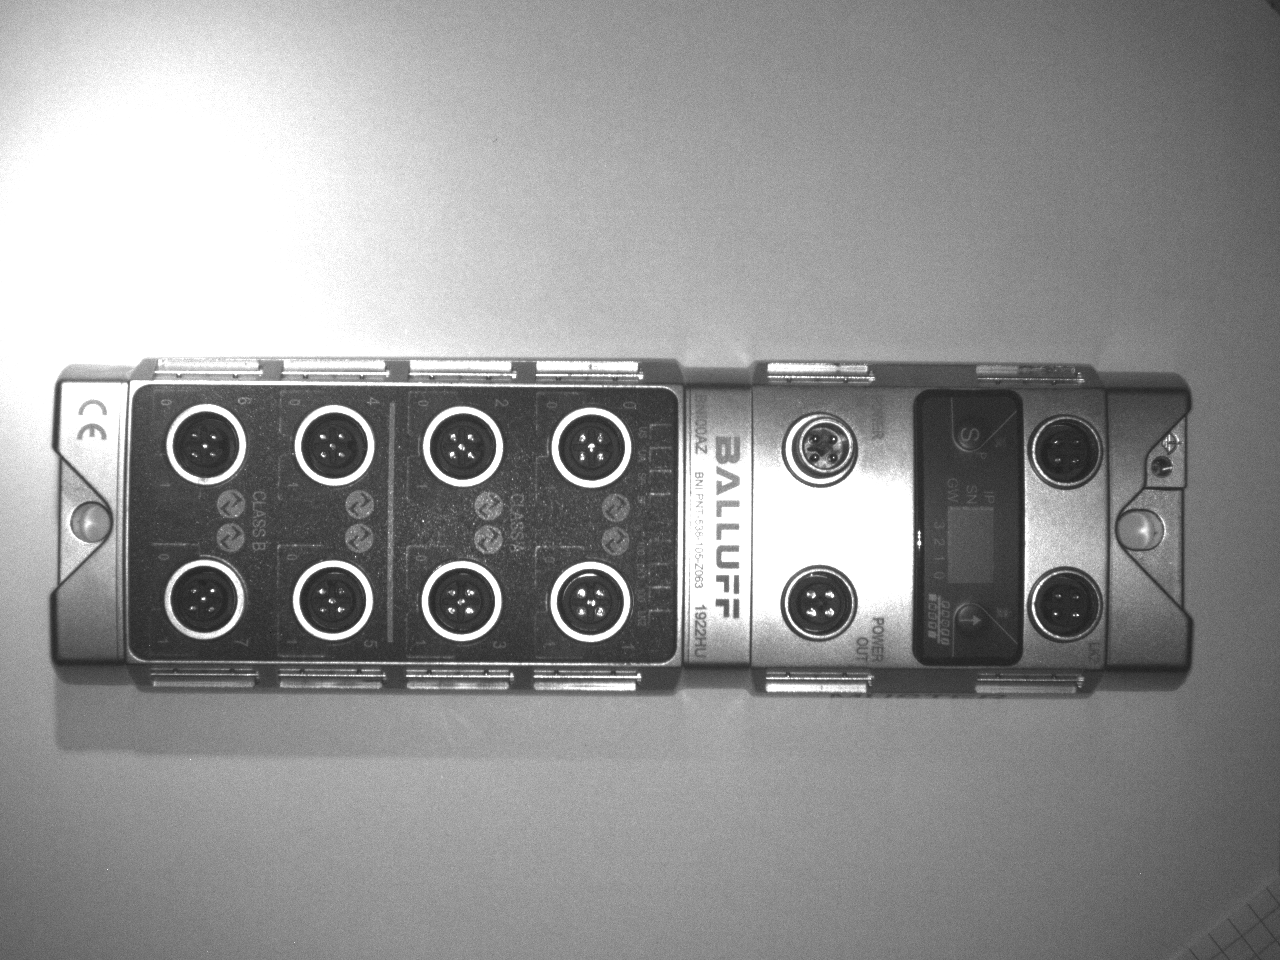
\includegraphics[scale=0.15]{../media/BNI-influence-right-OK.png}
            \caption{OK BNI with right inclination}
        \end{subfigure}
        \hfill
        \begin{subfigure}[b]{0.45\textwidth}
            \centering
            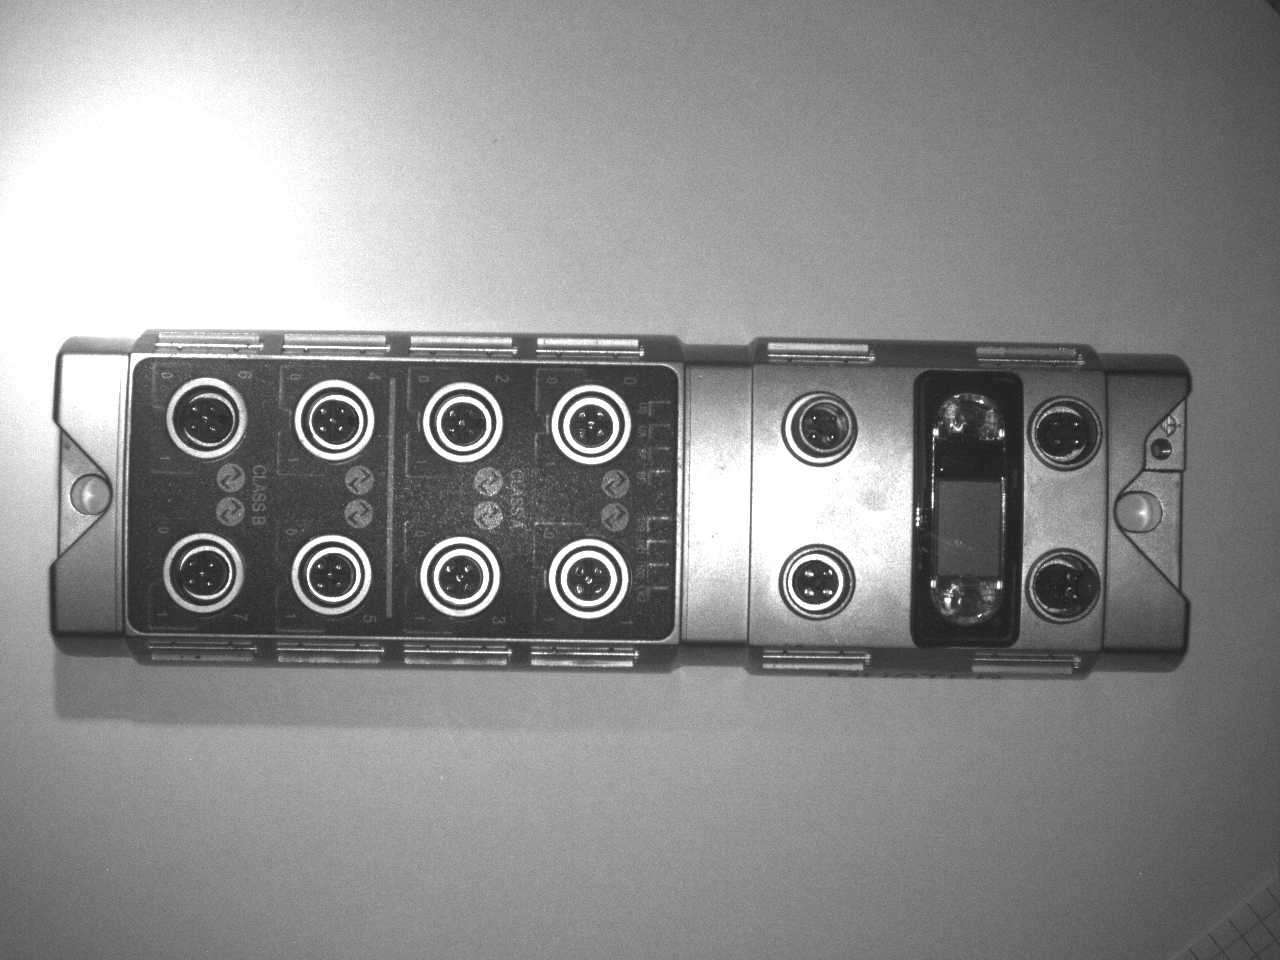
\includegraphics[scale=0.15]{../media/BNI-influence-right-NOK.png}
            \caption{NOK BNI with right inclination}
        \end{subfigure}
        \caption{Examples of BNIs affected by right inclination. (a) OK BNI and (b) NOK BNI with missing labels.}
        \label{fig:inclination_right}
    \end{figure}
    
    \item \textbf{Lighting:} Variations in lighting conditions were introduced, leading to shadows or overexposed areas on the BNIs. These lighting changes mimic real-world scenarios where inconsistent lighting can obscure defects or create reflections.
    
	The effects of lighting variations on the BNIs are demonstrated in Figure \ref{fig:lighting}, displaying both OK and NOK examples influenced by changes in illumination.
    \begin{figure}
        \centering
        \begin{subfigure}[b]{0.45\textwidth}
            \centering
            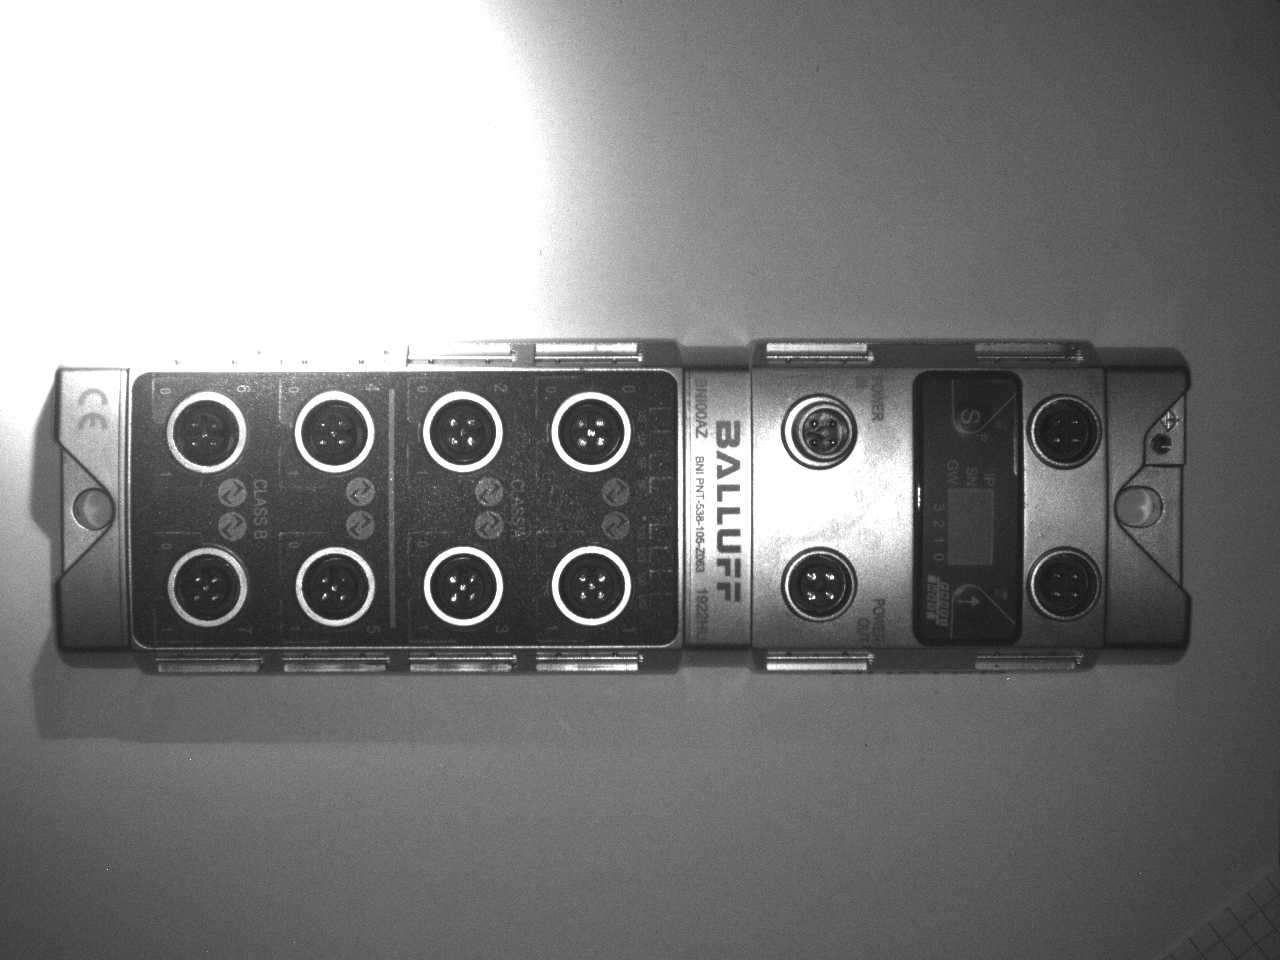
\includegraphics[scale=0.15]{../media/BNI-influence-lighting-OK.png}
            \caption{OK BNI under varied lighting}
        \end{subfigure}
        \hfill
        \begin{subfigure}[b]{0.45\textwidth}
            \centering
            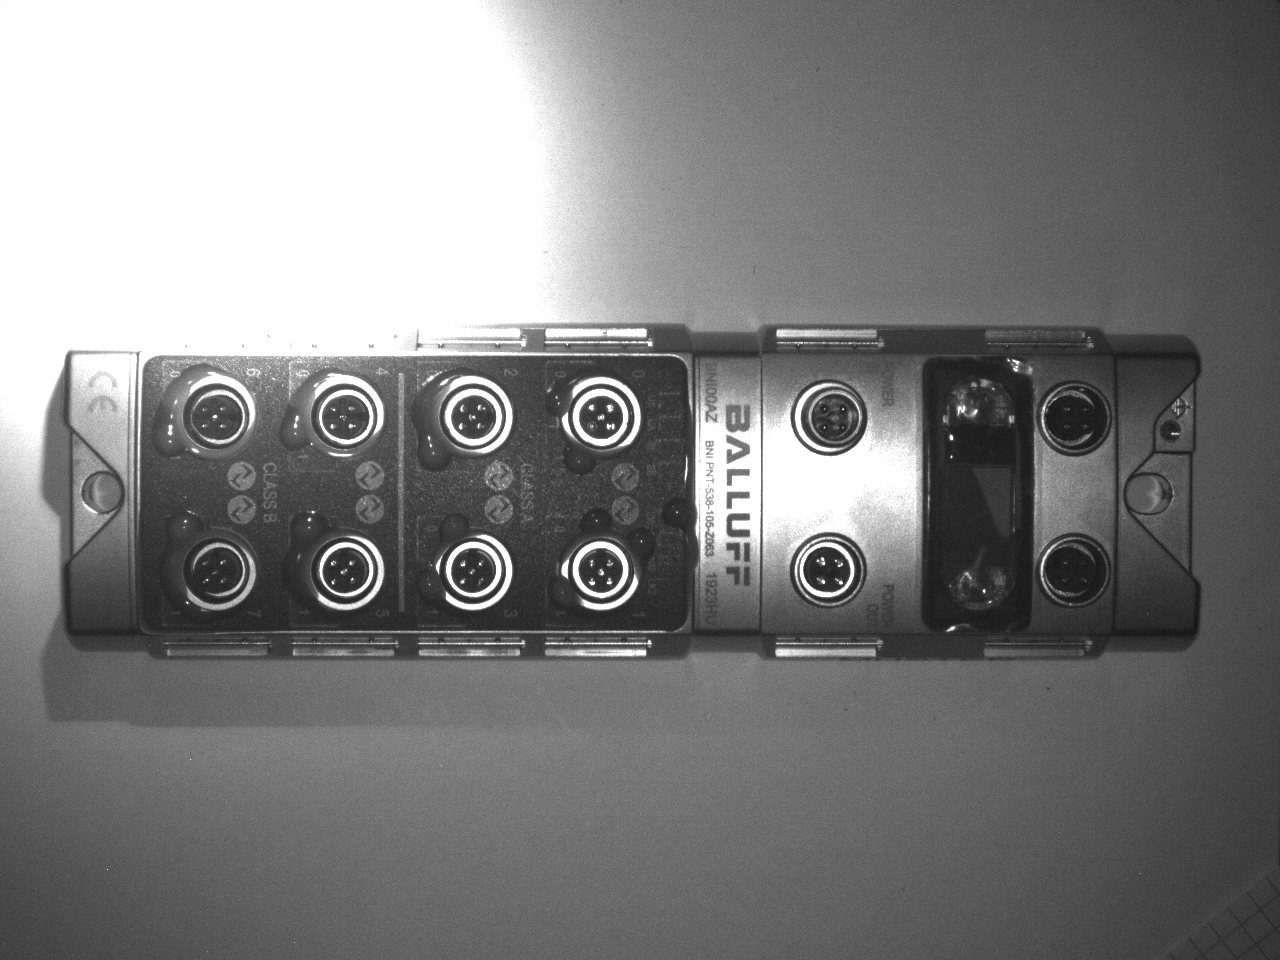
\includegraphics[scale=0.15]{../media/BNI-influence-lighting-NOK.png}
            \caption{NOK BNI under varied lighting}
        \end{subfigure}
        \caption{Examples of BNIs affected by varied lighting. (a) OK BNI and (b) NOK BNI showing traces of solidified epoxy resin.}
        \label{fig:lighting}
    \end{figure}

    \item \textbf{Random Object Placement:} BNIs were positioned randomly within the image frame or at unusual angles, leading to inconsistency in their placement. This can confuse anomaly detection models that rely on uniform object positioning to identify defects.
    
	Figure \ref{fig:random_placement} shows how random object placement affects the BNIs, highlighting both OK and NOK images impacted by this irregular positioning.
    \begin{figure}
        \centering
        \begin{subfigure}[b]{0.45\textwidth}
            \centering
            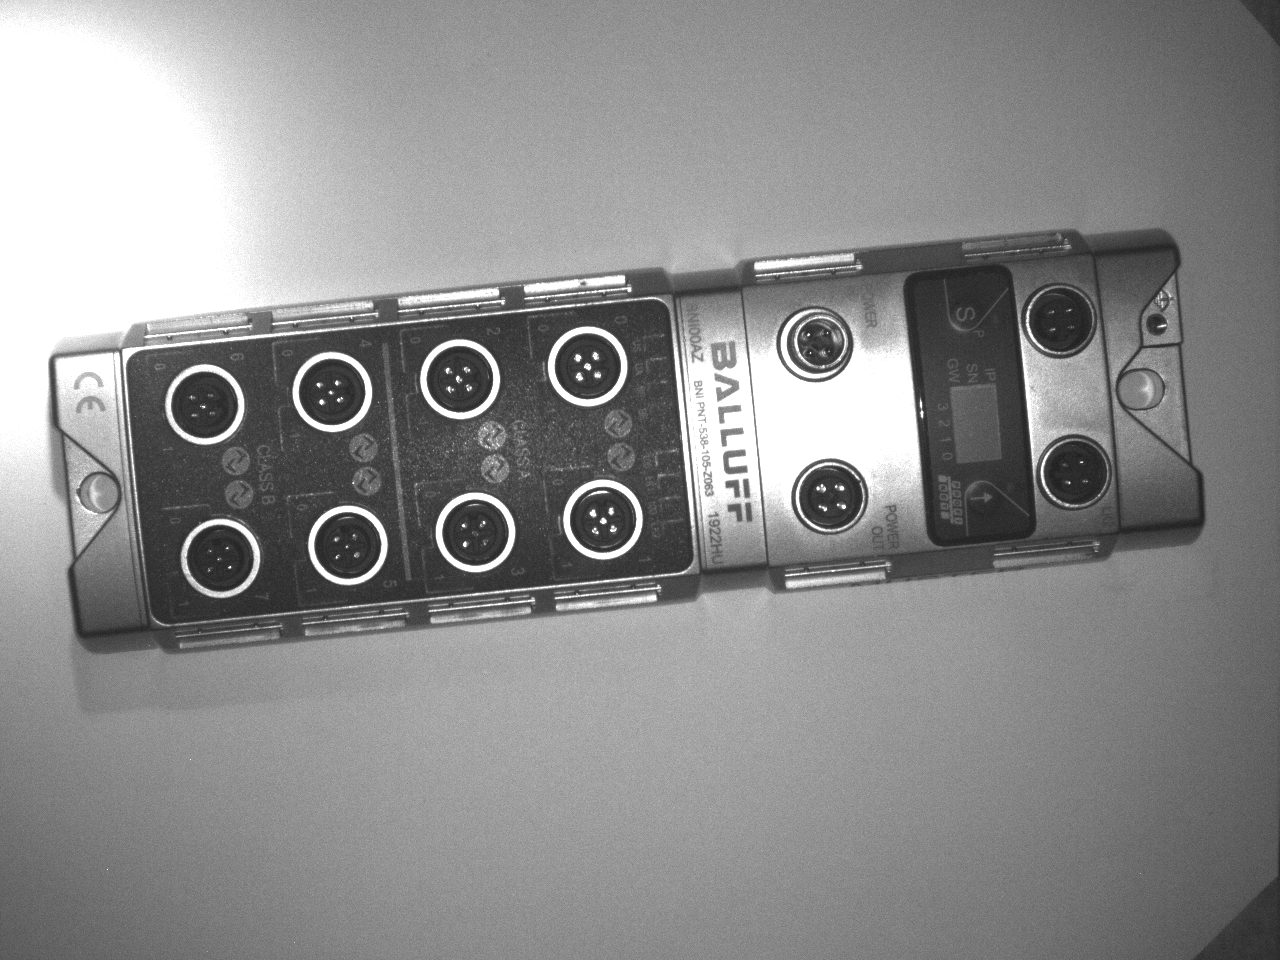
\includegraphics[scale=0.15]{../media/BNI-influence-random-OK.png}
            \caption{OK BNI with random placement}
        \end{subfigure}
        \hfill
        \begin{subfigure}[b]{0.45\textwidth}
            \centering
            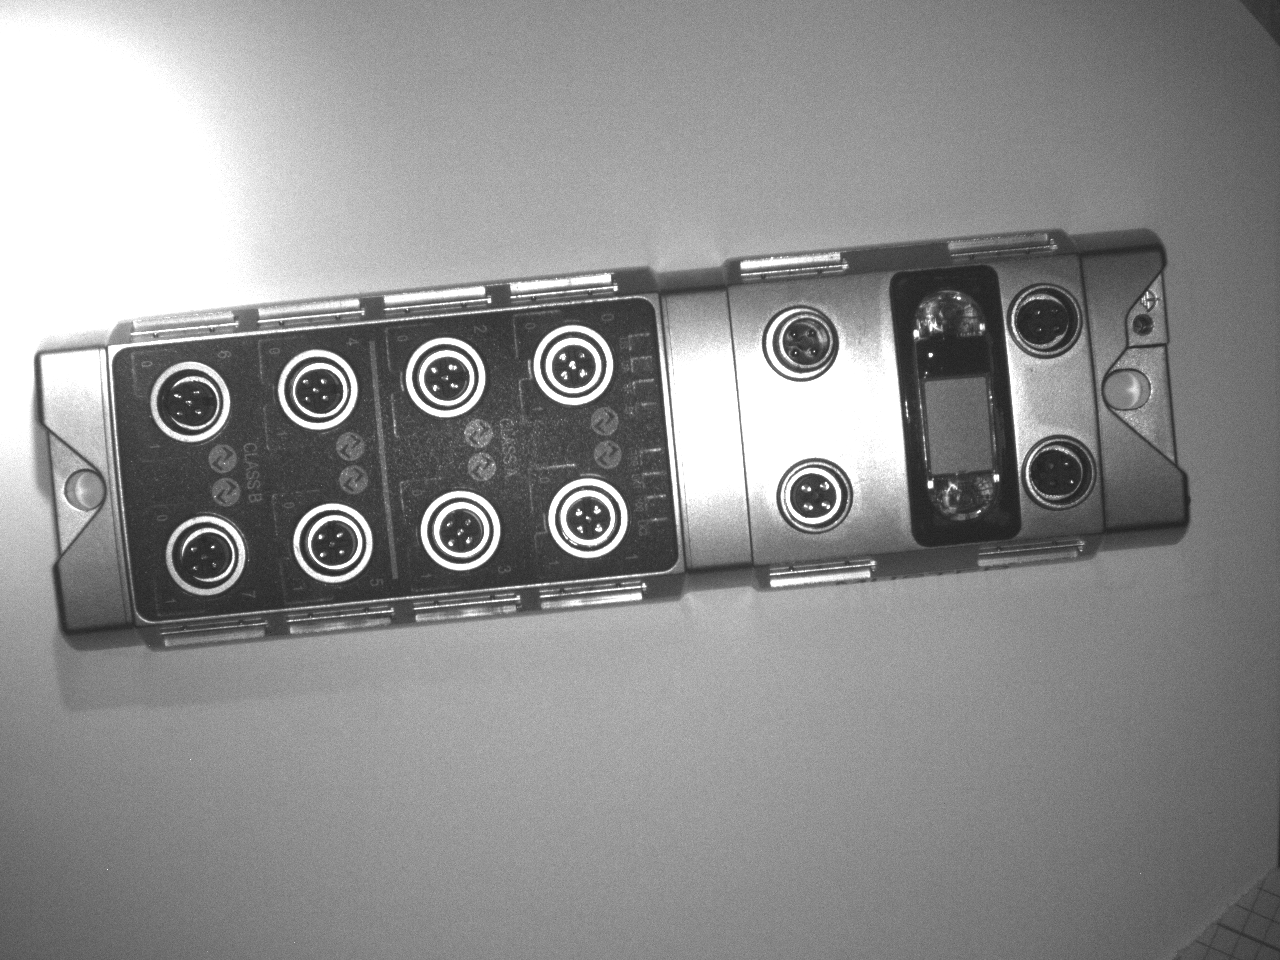
\includegraphics[scale=0.15]{../media/BNI-influence-random-NOK.png}
            \caption{NOK BNI with random placement}
        \end{subfigure}
        \caption{Examples of BNIs affected by random placement. (a) OK BNI and (b) NOK BNI where some labels are absent.}
        \label{fig:random_placement}
    \end{figure}
\end{enumerate}
\subsection{PCB Dataset}
PCBs are crucial components in electronic devices, providing the framework for mounting and connecting electronic components. The PCB dataset includes both OK and NOK images captured under two different setups: optimal conditions and conditions influenced by additional lighting. The details of the dataset size are summarized in Table~\ref{tab:pcb-dataset}.
\begin{table}
    \centering
    \caption{Printed Circuit Boards (PCB) Dataset Summary}
    \label{tab:pcb-dataset}
    \begin{tabular}{lcc}
        \toprule
        \textbf{Condition} & \textbf{Optimal Setup} & \textbf{Bad Influences} \\ 
        \midrule
        OK Images          & 54                     & 20                      \\ 
        NOK Images         & 20                     & 14                      \\ 
        \bottomrule
    \end{tabular}
\end{table}


Figure~\ref{fig:pcb_combined} illustrates the PCB images: (a) and (b) presents the OK and NOK PCBs under optimal conditions, showcasing the expected quality and visible defects, respectively. (c) and (d) displays the OK and NOK PCBs under the setup with added lighting, which may affect the clarity and assessment of the images.
\begin{figure}
    \centering
    \begin{subfigure}[b]{0.45\textwidth}
        \centering
        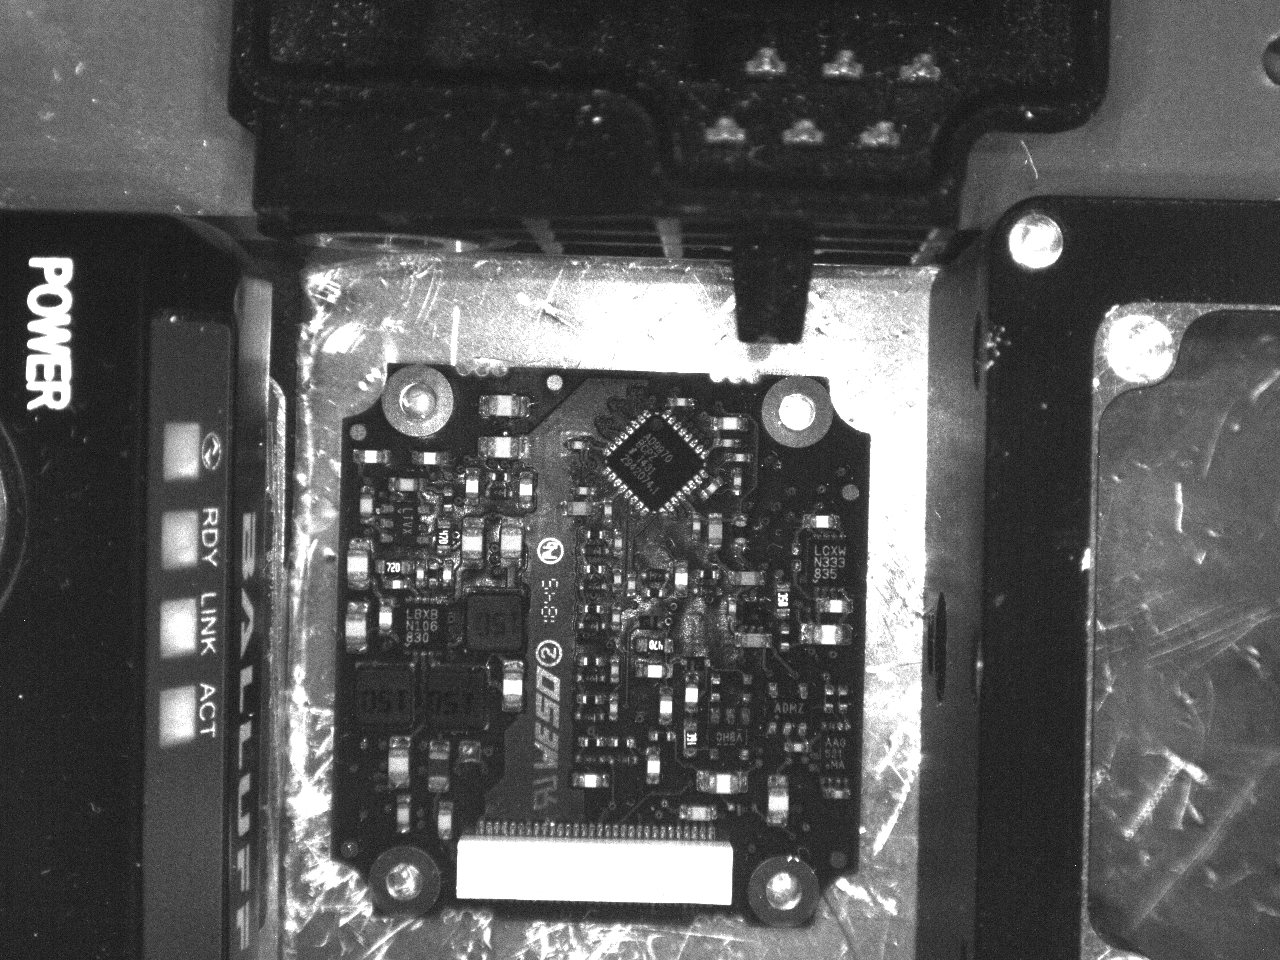
\includegraphics[scale=0.15]{../media/PCB-optimal-OK.png}
        \caption{OK PCB under optimal conditions}
        \label{fig:pcb_optimal_ok}
    \end{subfigure}
    \hfill
    \begin{subfigure}[b]{0.45\textwidth}
        \centering
        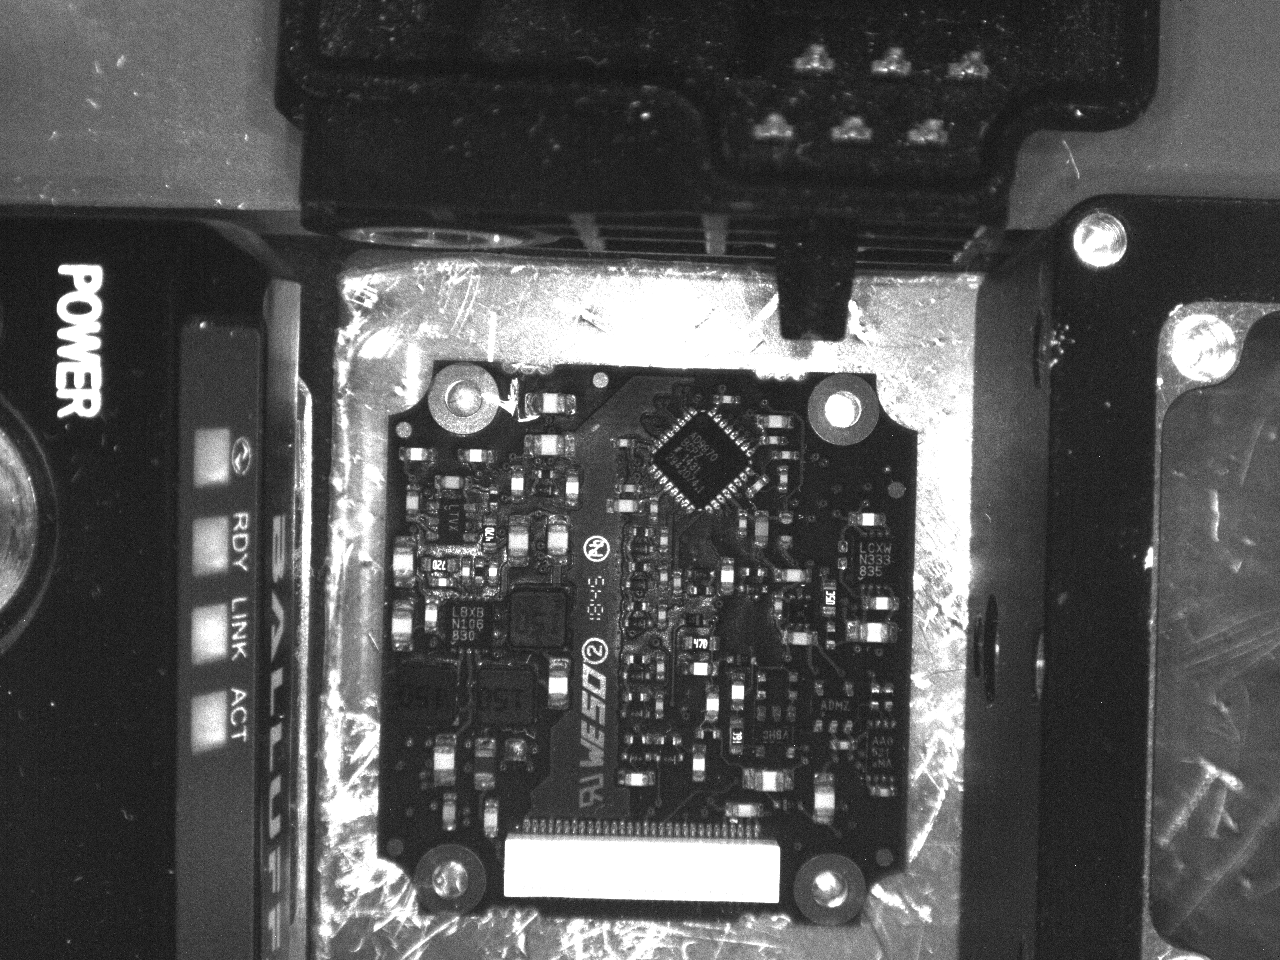
\includegraphics[scale=0.15]{../media/PCB-optimal-NOK.png}
        \caption{NOK PCB under optimal conditions}
        \label{fig:pcb_optimal_nok}
    \end{subfigure}
    \hfill
    \begin{subfigure}[b]{0.45\textwidth}
        \centering
        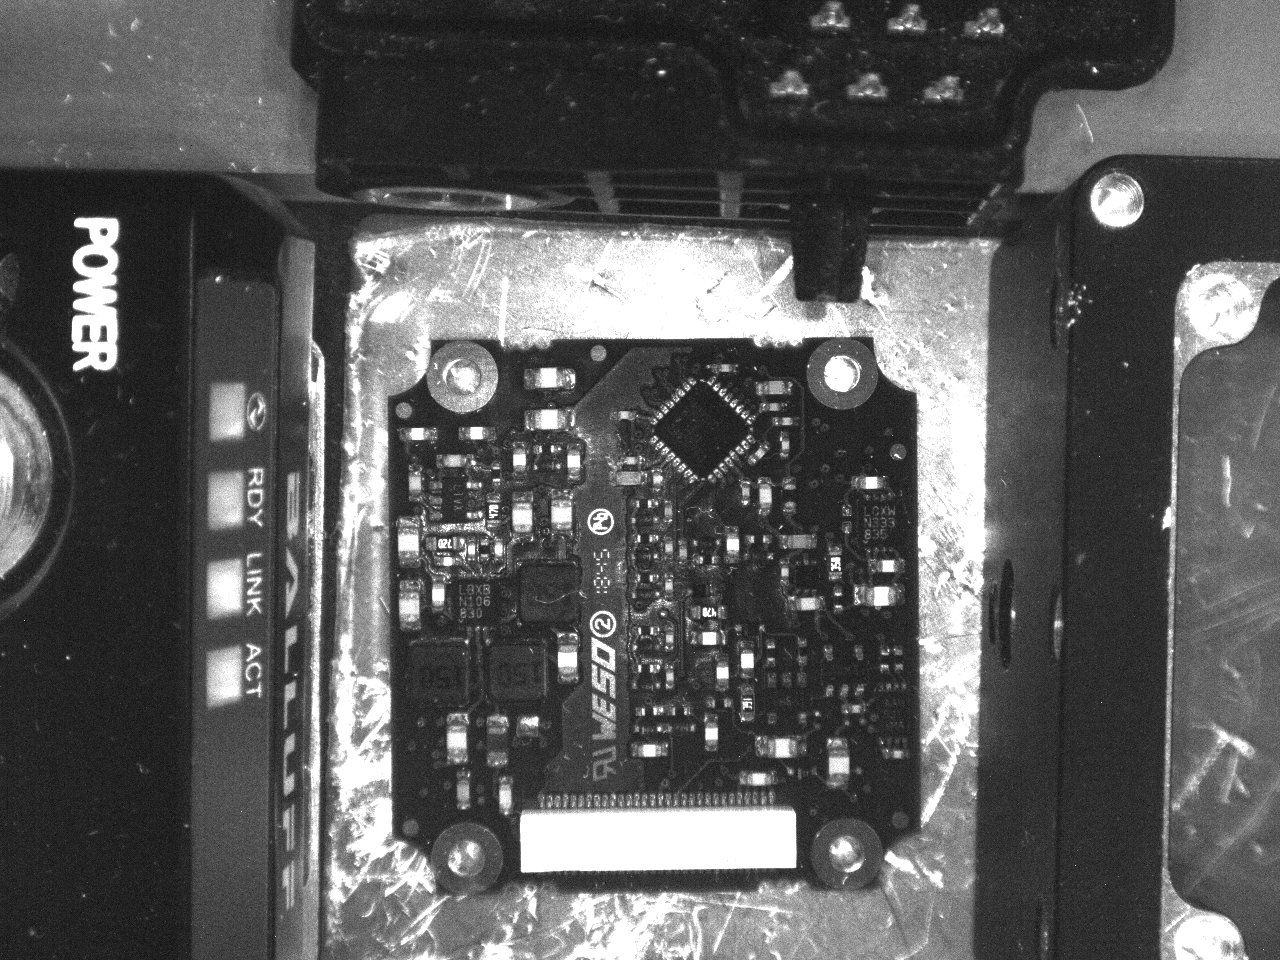
\includegraphics[scale=0.15]{../media/PCB-influence-OK.png}
        \caption{OK PCB under bad influence setup}
        \label{fig:pcb_bad_influence_ok}
    \end{subfigure}
    \hfill
    \begin{subfigure}[b]{0.45\textwidth}
        \centering
        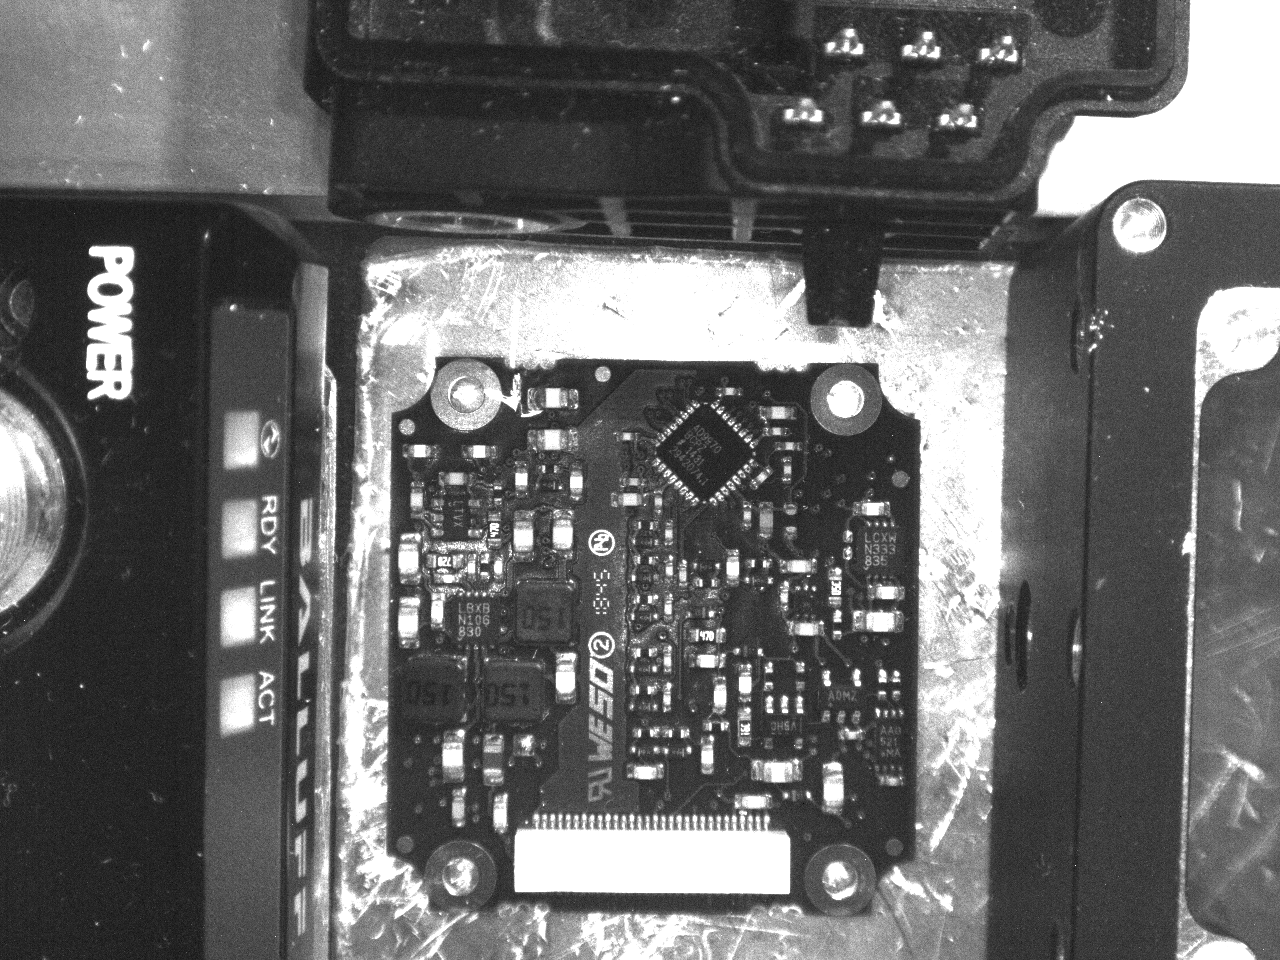
\includegraphics[scale=0.15]{../media/PCB-influence-NOK.png}
        \caption{NOK PCB under bad influence setup}
        \label{fig:pcb_bad_influence_nok}
    \end{subfigure}
    \caption{Examples of PCBs captured under different setups: (a) OK PCB under optimal conditions, (b) NOK PCB under optimal conditions, (c) OK PCB under bad influence setup with additional lighting, and (d) NOK PCB under bad influence setup. The added lighting may impact the visual assessment of the PCB quality.}
    \label{fig:pcb_combined}
\end{figure}
\section{Methods}
\subsection{Model Selection}
To improve the performance of the anomaly detection system, it was essential to train the model on a dataset that included various camera-induced influences such as shadow effects, lighting variations, plexiglas reflections, and random placement of objects. While real data under both optimal and influenced conditions were collected, the need arose to synthetically generate additional images that captured these artifacts. This was necessary to ensure that the anomaly detector could generalize effectively to the variations in the production environment.

Given the nature of this task, an image-to-image translation approach was selected as the most suitable method for generating these synthetic artifacts. While Pix2Pix~\cite{isola2017image} is a popular model for image translation tasks, it relies on paired datasets, which were unavailable in this case. Therefore, \textbf{CycleGAN}, introduced by Jun-Yan Zhu \textit{et al.} (2017)~\cite{zhu2017unpaired}, was chosen for its ability to perform unpaired image translation. A detailed explanation of CycleGAN is provided in Chapter~\ref{sec:cyclegan}.

Additionally, \textbf{Stable Diffusion} was used to enhance the generation of synthetic images. Stable Diffusion, a more recent deep learning model based on diffusion processes, was employed for its ability to generate highly realistic images with a broader range of variations in image quality. This model allowed for the refinement of synthetic images by controlling the level of noise and generating realistic variations under influenced conditions. The methodology and technical details of Stable Diffusion are covered in Chapter~\ref{sec:stable_diffusion}.
\subsection{CycleGAN Method}
\label{sec:cyclegan}
The CycleGAN architecture consists of two generator models and two discriminator models, following a similar architecture as described in the original paper~\cite{zhu2017unpaired}, facilitating the translation of images between two distinct domains: Domain-A and Domain-B. This subsection details the overall workflow, including data loading and preprocessing, data augmentation, model architecture, and training procedure.

\textbf{Data Loading and Preprocessing}

For the CycleGAN model implementation, the datasets chosen were the Nuts and Candles datasets, as they provide a sufficiently large number of images compared to the BNI and PCB datasets. Only the OK images from these datasets were utilized for training the CycleGAN model, while the NOK images will be employed later in the evaluation phase using the anomaly detection model.

The Nuts Dataset consists of 457 OK images, comprising:
\begin{itemize}
    \item \textbf{Domain A (Optimal)}: 152 images
    \item \textbf{Domain B (with bad influences)}: 305 images
\end{itemize}

The Candles Dataset includes 279 OK images, with:
\begin{itemize}
    \item \textbf{Domain A (Optimal)}: 145 images
    \item \textbf{Domain B (with bad influences)}: 134 images
\end{itemize}

Images were originally in Bitmap (BMP) format with a resolution of 1280x960. The generator and discriminator models used in this work are particularly large, with the generator containing approximately \textasciitilde 35 million parameters and the discriminator consisting of around \textasciitilde 2.8 million parameters. To handle such computational demands efficiently, the images were resized to 256x256 pixels and converted to Portable Network Graphics (PNG) format, ensuring compatibility with the input requirements of the models while optimizing memory usage and processing speed. The experiments were primarily conducted on the Nuts dataset due to its well-defined influences, allowing for more precise image translation.

\textbf{Data Augmentation}

The CycleGAN model utilized for this task contained approximately 38 million parameters, which posed the risk of overfitting, given the relatively small dataset size. To mitigate this, standard data augmentation techniques were applied using \texttt{ImageDataGenerator}~\cite{tensorflow_imagedatagenerator}. The following augmentations were implemented:

\begin{enumerate}
    \item Horizontal flipping
    \item Vertical flipping
    \item Rotation in the range [-10°, +10°]
    \item Width shift in the range of 0.1
    \item Height shift in the range of 0.1
\end{enumerate}
\begin{figure}
    \centering
    \begin{subfigure}[b]{0.45\textwidth}
        \centering
        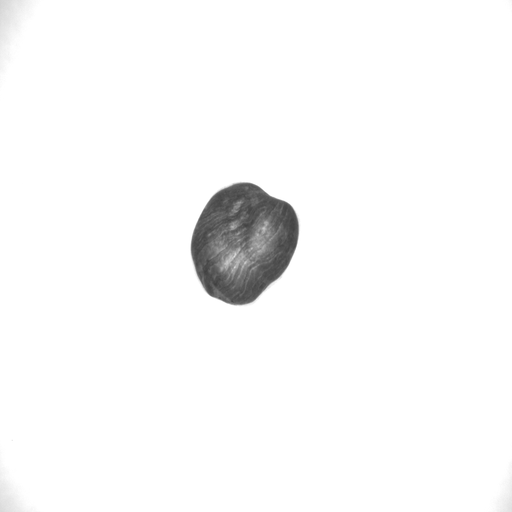
\includegraphics[scale=0.15]{../media/Original1.png} % Replace with the path to your original image
        \caption*{(a)}
    \end{subfigure}
    \hfill
    \begin{subfigure}[b]{0.45\textwidth}
        \centering
        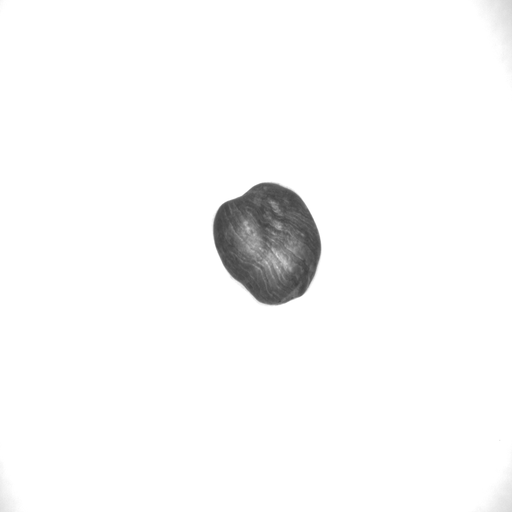
\includegraphics[scale=0.15]{../media/augmented_horizontal_flip.png} % Replace with the path to your augmented image
        \caption*{(b)}
    \end{subfigure}
    \caption{(a) The original nut image and (b) the augmented nut image with a horizontal flip applied.}
    \label{fig:nut_comparison}
\end{figure}

Figure~\ref{fig:nut_comparison} shows an example of an original nut image alongside its augmented version, where a horizontal flip has been applied.
These transformations were selected to ensure that they would not adversely affect the translation task. However, despite these augmentation strategies, the performance remained unaffected. It is crucial to note that the transformations only modify the geometry of the images without impacting the underlying information, which may limit the model's ability to learn effective translations.

\textbf{Model Architecture}

\begin{enumerate}
    \item \textbf{Generator Models}:
    \begin{itemize}
        \item \textbf{Generator-A}: This generator is responsible for creating images in Domain-A(Optimal). It takes images from Domain-B as input, performing image translation conditioned on these images. The architecture follows an encoder-decoder framework, starting with a convolutional layer that downscales the input. This is followed by a series of \textbf{nine residual blocks} for 256×256 input images, consisting two convolutional layers with 3×3 filters. Each layer uses Instance Normalization to standardize the inputs, helping the model generalize better to different domains. The stride is set to 1×1, ensuring that the spatial dimensions of the input are preserved. The input to each residual block is added back to the output, creating a skip connection that allows the network to retain low-level features while learning more complex ones. Importantly, the second convolutional layer does not use a ReLU activation, following the official CycleGAN paper~\cite{zhu2017unpaired} implementation for better image quality. The decoder then upsamples the features through transposed convolutional layers to produce the final output image. Detailed generator architecture is provided in Appendix~\ref{appendix:generator_model}.
        \item \textbf{Generator-B}: Conversely, Generator-B generates images in Domain-B(with bad influences) and takes images from Domain-A as input. It uses the same architectural principles as Generator-A, ensuring a consistent translation process.
    \end{itemize}

    The image translation processes can be illustrated as follows:

    \begin{align*}
    \text{Domain-B} & \xrightarrow{\text{Generator-A}} \text{Domain-A} \\
    \text{Domain-A} & \xrightarrow{\text{Generator-B}} \text{Domain-B}
    \end{align*}

    \item \textbf{Discriminator Models}:
    Each generator is paired with a corresponding discriminator:
    \begin{itemize}
        \item \textbf{Discriminator-A}: This model evaluates real images from Domain-A alongside the images generated by Generator-A, predicting whether each image is real or fake. It employs a PatchGAN approach~\cite{isola2017image}, processing $70 \times 70$ image patches with several convolutional layers, Instance Normalization, and LeakyReLU activations. The final layer outputs a probability map indicating the likelihood of each patch being real. An in-depth description of the generator architecture can be found in Appendix~\ref{appendix:discriminator_model}. 
        \item \textbf{Discriminator-B}: Similarly, this discriminator assesses real images from Domain-B and those produced by Generator-B. It shares the same network architecture as Discriminator-A, ensuring consistency in evaluations.
    \end{itemize}

    The interactions can be represented as:

    \begin{align*}
    \text{Domain-A} & \xrightarrow{\text{Discriminator-A}} [\text{Real/Fake}] \\
    \text{Domain-B} & \xrightarrow{\text{Generator-A}} \text{Discriminator-A} \xrightarrow{} [\text{Real/Fake}]
    \end{align*}

    \begin{align*}
    \text{Domain-B} & \xrightarrow{\text{Discriminator-B}} [\text{Real/Fake}] \\
    \text{Domain-A} & \xrightarrow{\text{Generator-B}} \text{Discriminator-B} \xrightarrow{} [\text{Real/Fake}]
    \end{align*}

    \item \textbf{Composite Model}: The composite model of CycleGAN leverages multiple loss components to enable effective image translation between two unpaired domains. The main loss components include:

		\begin{itemize}
				\item \textbf{Adversarial Loss:} This loss is central to the adversarial training process. The generators are tasked with creating images that can fool the discriminators into classifying them as real. Simultaneously, the discriminators aim to distinguish between real and generated images. The adversarial loss is responsible for improving the generator’s ability to create realistic images and the discriminator’s ability to identify fakes. It uses the L2 distance between the model's output and the target (real or fake).

				\textit{Adversarial Training Illustration:}
				\begin{align*}
				\text{Domain-A} & \xrightarrow{\text{Generator-B}} \text{Domain-B} \xrightarrow{\text{Discriminator-B}} [\text{real/fake}] \\
				\text{Domain-B} & \xrightarrow{\text{Generator-A}} \text{Domain-A} \xrightarrow{\text{Discriminator-A}} [\text{real/fake}]
				\end{align*}

				\item \textbf{Cycle Consistency Loss:} Cycle consistency ensures that if an image is translated from one domain to another and then back to the original domain, it should closely resemble the original image. This helps preserve the structure and content of the input images during translation. The cycle consistency loss is calculated as the L1 distance between the original and reconstructed images.

				\textit{Cycle A → B → A:}
				\begin{align*}
				\text{Domain-A} & \xrightarrow{\text{Generator-B}} \text{Domain-B} \xrightarrow{\text{Generator-A}} \text{Domain-A}
				\end{align*}

				\textit{Cycle B → A → B:}
				\begin{align*}
				\text{Domain-B} & \xrightarrow{\text{Generator-A}} \text{Domain-A} \xrightarrow{\text{Generator-B}} \text{Domain-B}
				\end{align*}

				\item \textbf{Identity Mapping Loss (Optional):} Identity mapping is employed to preserve domain-specific properties. When an image from a domain is passed through its corresponding generator, the output should remain unchanged. This is particularly useful for tasks that require maintaining the color profiles of images. The identity loss is calculated as the L1 distance between the input and output image.

				\textit{Identity Mapping for Domain-A:}
				\begin{align*}
				\text{Domain-A} & \xrightarrow{\text{Generator-A}} \text{Domain-A}
				\end{align*}

				\textit{Identity Mapping for Domain-B:}
				\begin{align*}
				\text{Domain-B} & \xrightarrow{\text{Generator-B}} \text{Domain-B}
				\end{align*}
		\end{itemize}

		These losses work together to ensure that the generators produce realistic images, preserve the structure of the original input, and maintain consistency across domains.
\end{enumerate}
\subsubsection{Training Procedure}

The CycleGAN model is trained to perform image-to-image translation from Domain A (optimal setup) to Domain B (setup with bad influences). The training process minimizes a combined loss function, which includes the adversarial loss, cycle-consistency loss, and identity loss. The generator \( G_{A \to B} \) is optimized through the composite model, while the discriminators \( D_A \) and \( D_B \) distinguish between real and generated images.

The training process runs for \( N_{epoch} = 100 \) epochs, with a batch size \( B = 1 \). The number of training steps per epoch is determined by the total number of images in the dataset, i.e., \( N_{steps} = \frac{N_{images}}{B} \), where \( N_{images} \) is the size of the Domain A dataset. For each step, real images from Domain A and Domain B are sampled, and fake images are generated by the generators. Discriminators are trained on both real and fake images to distinguish them, while the generator \( G_{A \to B} \) is trained to fool the discriminator.

An image pool is maintained for the discriminators to stabilize the training, where a set of 50 fake images is used to probabilistically update the discriminator. Plots of generated images are visualized during training to monitor the generator's performance, and models are saved periodically. After training, the model is selected based on iterations where the generated images appear visually appealing, allowing for the generation of new images from the training dataset.

The following table summarizes the hyperparameters used in the training procedure:

\begin{table}
    \centering
    \caption{Training Hyperparameters}
    \label{tab:hyperparameters}
    \begin{tabularx}{\textwidth}{XcX} % Change to use tabularx
        \toprule
        \textbf{Hyperparameter} & \textbf{Value} & \textbf{Description} \\ 
        \midrule
        Epochs & 100 & Total number of training epochs \\ 
        Batch size & 1 & Number of images processed per step \\
        Learning rate(Generator) & 0.0002 & Learning rate for the generator \\
        Learning rate(Discriminator) & 0.0002 & Learning rate for the discriminators \\
        Momentum (\( \beta_1 \)) & 0.5 & Momentum term for the Adam optimizer \\
        Cycle-consistency loss & 10x adversarial loss & Weight assigned to the cycle-consistency loss \\
        Identity loss & 5x cycle-consistency loss & Weight assigned to the identity loss \\
        Image pool size & 50 & Number of fake images stored in the image pool \\
        Training steps per epoch & \( \frac{N_{images}}{B} \) & Number of training steps per epoch based on dataset size \\ 
        \bottomrule
    \end{tabularx}
\end{table}

The goal is to achieve stable adversarial training where the generator produces realistic images of Domain B and the discriminators cannot easily distinguish between real and generated images.

\subsection{Stable Diffusion WebUI}
\label{sec:stable_diffusion}

Stable Diffusion WebUI, particularly the \texttt{AUTOMATIC1111} version, offers an easy-to-use interface for generating images using Stable Diffusion models. It supports a range of image manipulation tasks, including text-to-image, image-to-image, inpainting, and more, making it suitable for various creative and technical purposes. For this thesis, the Image-to-Image (\texttt{img2img}) functionality was used to generate synthetic images using real data. The requirements necessary for setting up the Stable Diffusion model are outlined in Appendix~\ref{appendix:stable_diffusion}.


\textbf{Using the img2img Tab in Stable Diffusion WebUI}

To generate synthetic images, begin by uploading a real image, for example an image of a Nut or Candle into the \texttt{img2img} tab. Once uploaded, select the appropriate checkpoint model, such as \texttt{sd\_xl\_base\_1.0\_0.9vae.safetensors} as shown in Figure~\ref{checkpoint}, ensuring compatibility with the model and task.
\begin{figure}
	\centering
	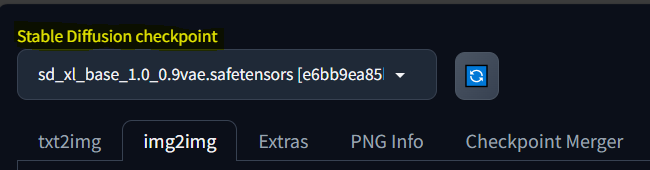
\includegraphics[scale=.9]{../media/stable_diffusion_checkpoint.PNG}
	\caption{Selecting Model Checkpoint}
	\label{checkpoint}
\end{figure}

\textbf{Key Settings and Configuration}

\begin{itemize}
    \item \textbf{Sampling Method (\(M_{\text{sam}}\)):} Determines the strategy for generating the image. \textit{DPM++ 2M Karras} was selected for its ability to decrease step sizes towards the end, enhancing image quality.
    
    \item \textbf{Sampling Steps (\(S_{\text{steps}}\)):} This controls the number of steps for transforming noise into an image. Higher step counts increase detail but also processing time. For this process, \(S_{\text{steps}} = 20\) were chosen, providing a balance between quality and efficiency.
    
    \item \textbf{Image Dimensions (\(D_{\text{img}}\)):} The width and height of the generated image are crucial for maintaining quality and consistency. A resolution of \(D_{\text{img}} = 512 \times 512\) was used, which is typical for Stable Diffusion models trained on this scale.
    
    \item \textbf{CFG Scale (\(s_{\text{cfg}}\)):} The CFG Scale indicates how strongly the generated image conforms to the input prompt; lower values allow for greater creativity. A CFG scale of \(s_{\text{cfg}} = 7\) was used to balance creative freedom with image fidelity.
    
    \item \textbf{Denoising Strength (\(s_{\text{den}}\)):} Defines how much change should be applied to the original image. At \(s_{\text{den}} = 0\), no changes occur, while at \(s_{\text{den}} = 1\), the image completely transforms. A value of \(s_{\text{den}} = 0.2\) was used to introduce some controlled variation while retaining key features of the original image.
    
    \item \textbf{Seed (\(s_{\text{seed}}\)):} This controls the randomness of the generation process. By setting the seed to \(s_{\text{seed}} = -1\), the system generates random images. Setting a specific value allows for consistent image reproduction.
    
    \item \textbf{Batch Count (\(B_{\text{count}}\)):} Specifies how many images are generated in one run. A count of \(B_{\text{count}} = 10\) ensures the generation of multiple variations for further evaluation.
    
    \item \textbf{Batch Size (\(B_{\text{size}}\)):} Determines how many images are processed simultaneously during generation. A batch size of \(B_{\text{size}} = 1\) was selected to maintain GPU efficiency while generating multiple images sequentially.
\end{itemize}

Figure~\ref{fig:webui_screenshot} shows the Stable Diffusion WebUI interface with the img2img tab and configuration settings for image generation.
\begin{figure}
	\centering
	\includegraphics[scale=.6]{../media/stable_diffusion_webui.PNG}
	\caption{Configuration settings in the Stable Diffusion WebUI for img2img}
	\label{fig:webui_screenshot}
\end{figure}
		
\subsection{Evaluation Metrics}
In image processing and analysis, assessing the quality of generated images is vital for understanding the performance of different algorithms and models. To achieve this, a variety of metrics are employed to quantify image quality, focusing on aspects such as similarity, distortion, and overall perceptual fidelity. Metrics like Oriented FAST and Rotated BRIEF(ORB), Structural Similarity Index(SSIM), Mean Squared Error(MSE), Peak Signal-to-Noise Ratio(PSNR), and perceptual loss using VGG16 facilitate comparisons between original and synthetic images, as well as the similarity between different generated images. This aids in optimizing techniques and ensuring that the generated results align with established quality standards. The following sections will explain these metrics in detail.

\textbf{ORB}

ORB by OpenCV is a feature detector and descriptor that efficiently identifies and describes keypoints in images, as developed by Ethan Rublee \textit{et al.} in their 2011 paper, \textbf{"ORB: An efficient alternative to SIFT or SURF"}~\cite{ORB}, making it particularly useful for image matching and object recognition tasks. The process begins with ORB detecting keypoints using the FAST algorithm, followed by generating binary descriptors through the BRIEF technique.

When comparing two images, ORB employs the Hamming distance metric to assess similarity by calculating the number of differing bits between the binary descriptors of matched features. A lower Hamming distance(\(d_H\)) indicates a closer match, which is essential for determining the degree of similarity between the images.

To enhance matching efficiency, ORB can be combined with a brute force matcher, which exhaustively compares each feature descriptor from one image with those from another to identify the best matches based on the lowest Hamming distance. An optimal Hamming distance threshold is crucial for improving matching accuracy; typically, values around \(d_H\) = 20 to 30 are considered ideal, as they indicate strong matches while minimizing the risk of false positives.

To calculate the overall ORB score, the number of good matches (i.e., matches with a Hamming distance below the threshold) is divided by the total number of matched descriptors. This score provides a quantitative measure of how similar the two images are overall, reflecting the effectiveness of the feature matching process.

\textbf{SSIM}

SSIM is a perceptual metric used to assess the quality of images by quantifying the degradation caused by processing tasks such as compression and transmission. Unlike traditional metrics that primarily rely on pixel-wise comparisons, SSIM evaluates changes in structural information, which reflects the way humans perceive visual information. The index incorporates three key components: luminance, contrast, and structural similarity.

\begin{itemize}
    \item \textbf{Luminance}: This component measures the brightness of the images. It calculates the average intensity of each image and compares them to determine how well the luminance levels align.
    
    \item \textbf{Contrast}: This aspect evaluates the contrast between the images, assessing how the variations in pixel intensity contribute to the overall perception of quality.
    
    \item \textbf{Structural Similarity}: This component examines the relationship between the pixels in both images, focusing on patterns of pixel intensities rather than individual pixel values.
\end{itemize}

The SSIM index produces a value between -1 and 1, where SSIM = 1 indicates perfect similarity between two images, and SSIM = -1 indicates significant differences. Due to its sensitivity to perceptual characteristics, SSIM is widely employed in various applications, including image compression, quality assessment, and computer vision tasks, as it correlates well with human visual perception.

\textbf{MSE}

MSE is a widely used metric to quantify the difference between the original and generated images. It calculates the average of the squares of the differences between corresponding pixel values. The formula for MSE is given by:

\begin{equation}
MSE = \frac{1}{N} \sum_{i=1}^{N} (I_{original}(i) - I_{generated}(i))^2
\end{equation}

where \( N \) is the total number of pixels, \( I_{original}(i) \) is the pixel value at position \( i \) in the original image, and \( I_{generated}(i) \) is the pixel value at the same position in the generated image.

A lower MSE value indicates a closer resemblance between the two images, meaning better image quality. Ideally, an MSE = 0 represents perfect similarity between the images. However, MSE can sometimes be misleading as it does not consider perceptual factors, meaning that images with similar MSE values may not necessarily appear similar to human observers.

\textbf{PSNR}

PSNR is another commonly used metric for assessing image quality, especially in the context of lossy compression. PSNR is derived from MSE and provides a measure of the maximum possible power of a signal (the original image) relative to the power of the noise (the error introduced by compression). The formula for PSNR is given by:

\begin{equation}
PSNR = 10 \cdot \log_{10}\left(\frac{MAX_I^2}{MSE}\right)
\end{equation}

where \( MAX_I \) is the maximum possible pixel value of the image (typically 255 for 8-bit images).

PSNR is expressed in decibels (dB), and a higher PSNR value indicates better image quality, as it signifies a lower level of noise. An optimum PSNR value is generally considered to be PSNR = 30 dB or higher for good quality images, with values above PSNR = 40 dB indicating very high quality. While PSNR is easy to compute and widely used, it also has limitations, as it does not align perfectly with human visual perception, and higher PSNR values do not always guarantee higher visual quality.

\textbf{Perceptual Loss using VGG16}

Perceptual loss measures the differences between two images based on high-level features extracted by a pre-trained deep convolutional neural network, specifically VGG16~\cite{VGG16}. Developed by Oxford's Visual Geometry Group, VGG16 consists of 16 layers, where the early layers focus on extracting low-level features (such as edges and textures), while the deeper layers capture high-level features (like shapes and object parts).

In the context of calculating perceptual loss between two images, the features from both the real and generated images are extracted using VGG16. The process involves loading the pre-trained model and preprocessing the images to match VGG16's input requirements. Once the features are extracted, the perceptual loss is computed by comparing these feature representations, providing a measure of similarity that aligns more closely with human visual perception. An optimal perceptual loss value is typically low, indicating a closer match between the images, which is essential for effective image quality assessment

\textbf{Comparing Two Sets of Images Using VGG16 Feature Extraction and a Classifier}

This method evaluates the similarity between two sets of images: real images and those generated by a model (Stable Diffusion). By employing the pre-trained network VGG16 as a feature extractor, this technique captures essential semantic information while focusing on high-level features instead of pixel-wise differences.

\textbf{Process Overview:}
\begin{enumerate}
    \item \textbf{Feature Extraction}: Real and generated images are preprocessed and fed into the VGG16 model to extract high-dimensional feature vectors that represent the content of each image. The feature maps produced by VGG16 are then flattened into 1D arrays to facilitate further analysis.

    \item \textbf{Feature Combination}: The extracted features from both sets are combined, with labels assigned (1 for real images and 0 for generated images) to facilitate classification.

    \item \textbf{Classifier Training}: A machine learning classifier, such as Logistic Regression or Random Forest, is trained on the combined feature set. The classifier attempts to find a hyperplane that effectively separates the high-dimensional space into two distinct regions: one representing real images and the other representing generated images. The dataset is divided into training, validation, and test sets to ensure comprehensive evaluation.

    \item \textbf{Model Evaluation}: The classifier's performance is measured using accuracy and ROC AUC metrics on the validation and test datasets. Additionally, confusion matrices are employed for performance visualization, providing insights into true positive, true negative, false positive, and false negative rates.

    \item \textbf{Dimensionality Reduction and Visualization}: To further analyze the feature vectors, Principal Component Analysis (PCA) is utilized for dimensionality reduction. This technique transforms the high-dimensional feature space into a lower-dimensional representation while preserving as much variance as possible. The reduced features allow for effective visualization of the distribution and clustering of images based on their labels, aiding in the interpretation of the classifier's performance and the inherent similarities or differences between the two sets of images.
\end{enumerate}

\subsection{Anomaly Detection on Nuts Dataset}
This section discusses the evaluation of an anomaly detection model using the Nuts dataset, which consists of images categorized into OK (good) and NOK (not okay) classes captured under various conditions. As summarized in Table~\ref{tab:nuts-dataset}, the dataset includes a variety of images captured under both optimal conditions and those affected by different influences. The evaluation involves three distinct approaches to training the model, each with a different composition of training datasets. The model's performance will be assessed using a consistent test dataset, with key metrics analyzed to gauge the effectiveness of each approach.

This test dataset as given in Table~\ref{tab:test-dataset-composition} comprises:

\begin{itemize}
    \item All 48 NOK images captured under optimal conditions.
    \item All 93 NOK images with bad influences.
    \item 31 OK images captured under optimal conditions (30\% of the total 152 OK images).
    \item 60 OK images with bad influences, covering each of the four variations: shadow, random placement, high gain factor, and plexiglas.
\end{itemize}

\begin{table} 
    \centering
    \caption{Test Dataset Composition}
    \label{tab:test-dataset-composition}
    \begin{tabular}{lc} % Change to remove vertical lines
        \toprule
        \textbf{Type} & \textbf{Number of Images} \\ 
        \midrule
        OK Optimal & 31 \\ 
        OK Bad Influences & 60 \\ 
        NOK Optimal & 48 \\ 
        NOK Bad Influences & 93 \\ 
        \midrule
        \textbf{Total} & 232 \\ 
        \bottomrule
    \end{tabular}
\end{table}

The following descriptions detail the training datasets utilized for each approach and how the model's performance was evaluated.

\textbf{First Approach: Training with Only Good Optimal Images}

In the first approach, only the 121 OK images captured under optimal conditions were used as the training dataset. No images with bad influences were included during training. The objective of this approach was to observe the anomaly detector’s performance when trained on ideal images and tested with both optimal and bad influence images in the test dataset.

Images used for training in the first approach is given in Table~\ref{tab:first-approach}.

\begin{table}
    \centering
    \caption{Training Dataset Composition for First Approach}
    \label{tab:first-approach}
    \begin{tabular}{lc} % Removed vertical lines
        \toprule
        \textbf{Category} & \textbf{Number of Images} \\ 
        \midrule
        OK Optimal (Real) & 121 \\ 
        \bottomrule
    \end{tabular}
\end{table}

\textbf{Second Approach: Adding Real Bad Influence Images}

In the second approach, the remaining 245 OK images with bad influences (from the total 305) were added to the 121 OK optimal images from the first approach. This aims to evaluate if the inclusion of real bad influence images improves the performance of the anomaly detector.

Images used for training in the second approach are provided in Table~\ref{tab:second-approach}.

\begin{table} 
    \centering
    \caption{Training Dataset Composition for Second Approach}
    \label{tab:second-approach}
    \begin{tabular}{lc} % Removed vertical lines
        \toprule
        \textbf{Category} & \textbf{Number of Images} \\ 
        \midrule
        OK Optimal (Real) & 121 \\ 
        OK Bad Influences (Real) & 245 \\ 
        \bottomrule
    \end{tabular}
\end{table}


\textbf{Third Approach: Incorporating Synthetic Bad Influence Images}

In the third approach, instead of using real bad influence images, 245 synthetically generated images (using Stable Diffusion) were added to the 121 OK optimal real images. This approach tests whether synthetically generated images can achieve similar results to real images in anomaly detection.

Images used for training in the third approach are listed in Table~\ref{tab:third-approach}

\begin{table} 
    \centering
    \caption{Training Dataset Composition for Third Approach}
    \label{tab:third-approach}
    \begin{tabular}{lc} % Removed vertical lines
        \toprule
        \textbf{Category} & \textbf{Number of Images} \\ 
        \midrule
        OK Optimal (Real) & 121 \\ 
        OK Bad Influences (Synthetic) & 245 \\ 
        \bottomrule
    \end{tabular}
\end{table}

\textbf{Implementation Details}

The implemented anomaly detection method utilizes a convolutional autoencoder to reconstruct input images and assess their similarity to the original data. A convolutional autoencoder learns efficient representations through an encoder-decoder architecture, compressing the input into a lower-dimensional latent space and reconstructing it from this representation.

The training dataset consists of images resized to 256x256 pixels and normalized to the range of [0, 1]. This dataset is shuffled and split into training (80\%) and validation (20\%) sets.

The convolutional autoencoder architecture varies slightly among the three approaches: Approach 1 employs a simpler design with fewer layers, featuring two convolutional layers in the encoder with 32 and 16 filters, and two corresponding layers in the decoder with 16 and 32 filters. In contrast, Approaches 2 and 3 each add an extra convolutional layer in the encoder with 64 filters and an additional corresponding layer in the decoder also with 64 filters, allowing for the capture of more complex features from the input data and enhancing feature extraction and reconstruction capabilities.

Training occurs over 100 epochs, utilizing mean squared error as the loss function. Both training and validation losses are monitored to ensure effective learning. After training, reconstruction errors for the validation set are computed to evaluate the model's performance in reconstructing normal images versus anomalous ones. A threshold for anomaly detection is established based on the 95th percentile of these reconstruction errors.

Finally, the model's effectiveness is evaluated on separate test datasets containing both normal and anomalous images. Metrics such as confusion matrices, accuracy, precision, recall, F1-score, and balanced accuracy are computed to provide a comprehensive assessment of all three approaches.

\chapter{Results and Discussions}
\label{chapter4}
This chapter presents the results and discussion of experiments conducted using CycleGAN on two datasets: Nuts and Candles. These datasets were selected due to their larger size compared to the PCB and BNI datasets, allowing for more robust evaluation of the CycleGAN model. The results for the Nuts dataset are presented first, followed by the Candles dataset. Throughout the discussion, specific challenges encountered during the training process across both datasets will be highlighted. Next, the results from Stable Diffusion are presented, focusing on the impact of denoising strength on the generated images. The generated images for all four datasets are then presented and discussed in terms of their quality and realism. Subsequently, key evaluation metrics are discussed to assess the image quality and similarity between the real and generated images. Finally, the performance of the anomaly detector was evaluated using the generated images from Stable Diffusion.
\section{CycleGAN Experiments}

\subsection{Experiments with Nuts Dataset}
\label{sec:cyclegan_nuts}
The experiments involving the Nuts dataset aimed to translate images from optimal setups to those influenced by various camera-induced factors. Specifically, this dataset encompasses four distinct types of influences: \textbf{Shadow}, \textbf{Random Placement}, \textbf{High Gain Factor}, and \textbf{Plexiglas Effect}, as discussed in Chapter~\ref{sec:nuts_dataset}.

Following this, the results presented are some of the intermediate results obtained during the training of the CycleGAN model. Certain hyperparameters, as detailed in Table~\ref{tab:hyperparameters}, were modified to evaluate their impact on the results. Intermediate results were saved after each epoch to facilitate the assessment of model performance throughout the training process, and any changes to hyperparameters for specific results will be noted.

\textbf{Shadow Effect}

Figure~\ref{fig:shadow_effect_result} illustrates the image translation from optimal setup to shadow effect, obtained during CycleGAN training at the 13th epoch. Figure~\ref{fig:shadow_effect_result} (a) presents five images from the optimal setup (Domain A) alongside the corresponding translated images that exhibit the shadow effect. Figure~\ref{fig:shadow_effect_result} (b) provides a reference image displaying the original shadow effect for comparison.

The translated images effectively capture the background and shadow characteristics seen in the reference image, with the Nuts appearing realistic. The hyperparameter settings for this experiment align with those outlined in Table~\ref{tab:hyperparameters}, indicating that the results were derived under the original configuration.

\begin{figure}
    \centering
    \begin{subfigure}[b]{0.85\textwidth}
        \centering
        \includegraphics[width=\textwidth]{../media/Shadow.png}
        \caption*{(a)}
    \end{subfigure}
    \hfill
    \begin{subfigure}[b]{0.25\textwidth}
        \centering
        \includegraphics[width=\textwidth]{../media/shadow_real.png}
        \caption*{(b)}
    \end{subfigure}
    \caption{Results of CycleGAN image translation showcasing the shadow effect. (a) Translated images from optimal setups. (b) Reference image of the original shadow effect.}
    \label{fig:shadow_effect_result}
\end{figure}

\textbf{High Gain Factor Effect}

Figure~\ref{fig:high_gain_factor_result} illustrates the impact of translating images from the optimal setup to those influenced by a high gain factor, captured during CycleGAN training at the 61st epoch. Figure~\ref{fig:high_gain_factor_result} (a) displays a series of images from the optimal setup, along with the corresponding translated images that exhibit the high gain factor effect. Figure~\ref{fig:high_gain_factor_result} (b) presents a real image as a reference highlighting the high gain factor effect. 

The results show a visible high gain factor effect, yet the realism in nut appearance is lacking, indicating that the translation process may not fully capture the nuances of the high gain factor influence. Again, the original model architecture, training procedure and same hyperparameter values as in Table~\ref{tab:hyperparameters} were used in this experiment.

\begin{figure}
    \centering
    \begin{subfigure}[b]{0.85\textwidth}
        \centering
        \includegraphics[width=\textwidth]{../media/high_gain.png}
        \caption*{(a)}
    \end{subfigure}
    \hfill
    \begin{subfigure}[b]{0.25\textwidth}
        \centering
        \includegraphics[width=\textwidth]{../media/high_gain_real.png}
        \caption*{(b)}
    \end{subfigure}
    \caption{Results of CycleGAN image translation highlighting the high gain factor effect. (a) Translated images from the optimal setup to images influenced by the high gain factor. (b) Reference image demonstrating the high gain factor effect.}
    \label{fig:high_gain_factor_result}
\end{figure}

\textbf{Plexiglas Effect}

Figure~\ref{fig:plexiglas_result} illustrates the results of translating images from the optimal setup to those with Plexiglas effect, obtained during CycleGAN training. Figure~\ref{fig:plexiglas_result} (a) presents the translated images showcasing the Plexiglas effect, while Figure~\ref{fig:plexiglas_result} (b) provides a reference image(real) that highlights the Plexiglas effect. 

For this experiment, the model complexity of both the generator and discriminator was reduced by simplifying their architecture. In the generator model, six ResNet blocks were used instead of the typical nine. Additionally, the learning rate of the discriminator was decreased from 0.0002 to 0.0001 to prevent it from becoming too dominant(loss value becoming zero) over the generator during training.

Despite the incorporation of these modifications, the results demonstrate only a minimal Plexiglas effect, lacking the intended visual appeal and clarity.
\begin{figure}
    \centering
    \begin{subfigure}[b]{0.85\textwidth}
        \centering
        \includegraphics[width=\textwidth]{../media/plexiglas.png}
        \caption*{(a)}
    \end{subfigure}
    \hfill
    \begin{subfigure}[b]{0.25\textwidth}
        \centering
        \includegraphics[width=\textwidth]{../media/plexiglas_real.png}
        \caption*{(b)}
    \end{subfigure}
    \caption{Results of CycleGAN image translation showcasing the Plexiglas effect. (a) Translated images from the optimal setup to images influenced by the Plexiglas effect. (b) Reference image illustrating the Plexiglas effect.}
    \label{fig:plexiglas_result}
\end{figure}

\textbf{Random Object Placement Effect}

One significant limitation of CycleGAN is its inherent inability to manage tasks that require specific spatial arrangements of objects within an image. When CycleGAN processes images from Domain A, it primarily focuses on preserving the core features of the original images while incorporating artifacts from Domain B. Consequently, any modifications made during this translation are constrained by the existing structures within Domain A.

In the context of random object placement effect, the challenge stems from the fact that the training dataset for Domain A does not include any images of Nuts arranged randomly. As a result, it lacks the capability to generate images that accurately depict the random placement of Nuts.

\subsection{Experiments with Candles Dataset}

The Candles dataset was utilized to examine the translation of images from optimal setups to those impacted by different environmental and camera-induced influences like \textbf{Scattered Sunlight}, \textbf{Random Object Placement}, \textbf{Camera Elevation (Up)}, and \textbf{Camera Elevation (Down)}, as discussed in Chapter~\ref{sec:candles_dataset}.

However, one of the challenges encountered with this dataset is that the visual differences between the various influences are not as pronounced as those observed in the Nuts dataset. This lack of clear distinction between influences made the analysis of generated images more difficult. As a result, the outputs produced by CycleGAN were harder to evaluate for accuracy and realism. Despite this, intermediate results saved after specific epochs during training revealed some promising translations, although the overall visual quality and differentiation were still not as satisfactory as expected.

The same hyperparameters, as detailed in Table~\ref{tab:hyperparameters}, were used for training the Candles dataset. The discriminator model's complexity was intentionally reduced to diminish its capacity for distinguishing between real and generated images. Specifically, the original discriminator architecture as in Appendix~\ref{appendix:discriminator_model} was modified by decreasing the number of convolutional filters in the initial layers from 64, 128, and 256 to 32, 64, and 128, respectively and by removing the final layer that utilized 512 filters. This simplification aimed to establish a better balance between the generator and discriminator during adversarial training, enhancing the generator's ability to produce more realistic outputs. Key components such as LeakyReLU activations and Instance Normalization were retained to stabilize training and improve convergence. Results were obtained at different epochs, with intermediate outputs saved throughout the training process, allowing for an assessment of the generated images over time. 

\textbf{Scattered Sunlight Effect}

Figure~\ref{fig:scattered_sunlight_result} illustrates the image translation from optimal setups to those influenced by scattered sunlight, obtained during CycleGAN training at the 56th epoch. 

\begin{figure}
    \centering
    \begin{subfigure}[b]{0.85\textwidth}
        \centering
        \includegraphics[width=\textwidth]{../media/candles_sunlight.png}
        \caption*{(a)}
    \end{subfigure}
    \hfill
    \begin{subfigure}[b]{0.25\textwidth}
        \centering
        \includegraphics[width=\textwidth]{../media/candles_sunlight_real.png}
        \caption*{(b)}
    \end{subfigure}
    \caption{Results of CycleGAN image translation showcasing the scattered sunlight effect. (a) Translated images from the optimal setup to images influenced by scattered sunlight. (b) Reference image illustrating the original scattered sunlight effect.}
    \label{fig:scattered_sunlight_result}
\end{figure}

\textbf{Camera Elevation(Down)}

Figure~\ref{fig:camera_elevation_down_result} illustrates the image translation from optimal setups to those influenced by camera elevation (down), obtained at the 67th epoch during training. 

\begin{figure}
    \centering
    \begin{subfigure}[b]{0.85\textwidth}
        \centering
        \includegraphics[width=\textwidth]{../media/candles_bright.png}
        \caption*{(a)}
    \end{subfigure}
    \hfill
    \begin{subfigure}[b]{0.25\textwidth}
        \centering
        \includegraphics[width=\textwidth]{../media/candles_bright_real.png}
        \caption*{(b)}
    \end{subfigure}
    \caption{Results of CycleGAN image translation showcasing the camera elevation (down) effect. (a) Translated images from the optimal setup to images influenced by camera elevation (down). (b) Reference image illustrating the original camera elevation (down) effect.}
    \label{fig:camera_elevation_down_result}
\end{figure}

\textbf{Camera Elevation(Up)}

Figure~\ref{fig:camera_elevation_up_result} illustrates the image translation from optimal setups to those influenced by camera elevation (up), obtained at the 84th epoch. 

\begin{figure}
    \centering
    \begin{subfigure}[b]{0.85\textwidth}
        \centering
        \includegraphics[width=\textwidth]{../media/candles_dark.png}
        \caption*{(a)}
    \end{subfigure}
    \hfill
    \begin{subfigure}[b]{0.25\textwidth}
        \centering
        \includegraphics[width=\textwidth]{../media/candles_dark_real.png}
        \caption*{(b)}
    \end{subfigure}
    \caption{Results of CycleGAN image translation showcasing the camera elevation (up) effect. (a) Translated images from the optimal setup to images influenced by camera elevation (up). (b) Reference image illustrating the original camera elevation (up) effect.}
    \label{fig:camera_elevation_up_result}
\end{figure}

\textbf{Analysis of Results}

The ~\textbf{Scattered Sunlight Effect} demonstrates the presence of bright sunlight; however, the generated images lack realism. In the case of ~\textbf{Camera Elevation (Down)}, the translated images appear slightly brighter, similar to the reference image, but do not exhibit the expected larger dimensions. Conversely, for ~\textbf{Camera Elevation (Up)}, the images appear darker but fail to convey the smaller size anticipated from this effect. As discussed in Chapter~\ref{sec:cyclegan_nuts}, CycleGAN preserves the integrity of images from Domain A while attempting to infuse artifacts from Domain B. This inherent characteristic explains the inability to achieve larger images in the case of Camera Elevation (Down) and smaller images in the case of Camera Elevation (Up). Additionally, the model is unable to generate the effect of ~\textbf{random object placement} for the same reasons. Overall, the results reveal that the generated images across all conditions are not particularly realistic, with candle threads not being generated clearly. Furthermore, the translated images in the Scattered Sunlight Effect, Camera Elevation (Down), and Camera Elevation (Up) show a notable similarity. This lack of diversity in outputs may suggest a potential modal collapse during training, leading to repetitive results across these conditions.

\subsection{Model Training Analysis}

The training process for the CycleGAN model can be evaluated by monitoring key losses over time. Three main loss functions were tracked to assess the performance: generator loss for A to B translation \( g\_loss\_AtoB \), and discriminator losses for real \( dB\_loss\_real \) and fake \( dB\_loss\_fake \) images in Domain B. The loss values showed similar trends while training with Nuts dataset and Candles dataset.

\textbf{Generator Loss for A to B Translation \( g\_loss\_AtoB \)}

The generator loss for A to B translation, shown in Figure~\ref{g_loss}, which is an average of three components: adversarial loss, identity loss, and cycle consistency loss and it gradually decreases over the course of training, as expected. This trend indicates that the generator is progressively improving its ability to produce realistic images of Domain B from Domain A. However, the training process shows fluctuations, with occasional spikes in the loss. This suggests that while the generator improves on average, there are certain points where the quality of the generated images temporarily drops. These fluctuations could be caused by instability in adversarial training, where the discriminator becomes briefly better at identifying fake images, forcing the generator to adapt. Additionally, the results do not improve in a steady manner, with epochs of high-quality results followed by others where the quality deteriorates. This inconsistency highlights the challenges associated with training GANs. Training was stopped when the loss values began to stabilize, indicating that further improvements in quality were minimal.
\begin{figure}
	\centering
	\includegraphics[scale=.51]{../media/g_loss_atob.png}
	\caption{Generator loss for A to B translation during training.}
	\label{g_loss}
\end{figure}

\textbf{Discriminator Losses}

The discriminator losses \( dB\_loss\_real \) and \( dB\_loss\_fake \), shown in Figure~\ref{fig:discriminator_losses}, initially decreases, but this is characterized by significant fluctuations rather than a smooth decline. Both loss curves experience abrupt spikes at various training epochs, indicating moments where the discriminator momentarily becomes better at distinguishing between real and generated images. Over time, both losses approach near-zero values, suggesting that the discriminator effectively learns to classify the images. However, despite this stabilization, the presence of sudden spikes demonstrates the ongoing challenges in adversarial training, where the balance between the generator and discriminator must be carefully managed to prevent either model from overpowering the other.
\begin{figure}
    \centering
    \begin{subfigure}[b]{1.0\textwidth}
        \includegraphics[width=\linewidth]{../media/dB_loss_real.png}
        \caption*{(a)}
        \label{fig:dB_loss_real}
    \end{subfigure}

    \begin{subfigure}[b]{1.0\textwidth}
        \includegraphics[width=\linewidth]{../media/dB_loss_fake.png}
        \caption*{(b)}
        \label{fig:dB_loss_fake}
    \end{subfigure}

    \caption{Discriminator losses during training: (a) loss for real images and (b) loss for fake images.}
    \label{fig:discriminator_losses}
\end{figure}

\subsection{Challenges Faced in CycleGAN Training}

While CycleGAN offers a powerful framework for unpaired image-to-image translation, several challenges emerged during training that impacted the quality and effectiveness of the generated images.

One of the key challenges encountered during the training of CycleGAN was~\textbf{mode collapse}. This problem, common in adversarial training, occurs when the generator produces a restricted range of outputs, failing to capture the full diversity of the training data. This results in repetitive or similar images regardless of the variations in the input, leading to a significant reduction in the overall output quality. As evidenced by the results, Candle images generated under different conditions, such as the Scattered Sunlight Effect and variations in Camera Elevation, exhibited striking similarities, suggesting that the model experienced mode collapse at various stages of training. This issue can often be attributed to the inherent instability of GAN architectures, wherein the delicate balance between the generator and discriminator is disrupted, causing the generator to latch onto specific modes of the data distribution while neglecting others. Factors such as discriminator overfitting and catastrophic forgetting can exacerbate this issue, ultimately hindering the generator's ability to produce varied and realistic outputs~\cite{modecollapse}.

Another significant challenge arose from the~\textbf{nature of the data}. Generative models, including CycleGAN, typically require large and diverse datasets to generalize well and produce varied results. However, in this case, the datasets were limited both in size and diversity. The Nuts and Candles datasets, although containing different samples, lacked significant variation in appearance. Many images of Nuts and Candles looked similar in terms of color, shape, and background. Although data augmentation techniques were applied to increase the diversity of the dataset, the inherent similarity between the images meant that these augmentations were not particularly helpful in improving the model’s ability to capture meaningful variations.

A further notable challenge was the~\textbf{instability of the training process}. Even though the losses showed a gradual decline over time, there were consistent fluctuations and occasional spikes in both generator and discriminator losses. This instability in the training dynamics is a characteristic of GAN models, where the adversarial nature of the training can lead to periods of rapid improvement followed by sudden regressions. In this case, the instability made it difficult to reach a point where the generator and discriminator could both perform optimally. This unstable training environment, combined with the limited and homogeneous data, ultimately hindered the ability of CycleGAN to produce realistic and varied outputs across different conditions.

\section{Stable Diffusion Experiments}

Initially, the goal was to introduce various camera influences into the images using generative models, particularly CycleGAN, for image-to-image translation. Although CycleGAN was capable of generating images with these camera influences, its limitations, including mode collapse and training instability, resulted in images that lacked the necessary quality and realism. As a result, these images could not be reliably used to train the anomaly detector effectively.

Consequently, Stable Diffusion, specifically the~\texttt{img2img} functionality was used to generate synthetic images. While direct image-to-image translation from optimal images to images with bad influences was not possible with Stable Diffusion, this approach allowed for the generation of synthetic images that incorporated the necessary camera influences. By uploading each real image with bad camera influence from the Nuts dataset and setting a low denoising strength (e.g., $s_{\text{den}} = 0.2$) and all the other configurations as mentioned in Chapter~\ref{sec:stable_diffusion}, it was possible to generate similar images with subtle variations in texture, which were considered more suitable for testing. This approach was applied to all the images from the Domain B dataset of Nuts, creating a set of synthetic images corresponding to each real image. These synthetic images were integrated into the anomaly detection process to test whether they could replicate the performance improvements observed when real images with bad influences were used.

Thus, while the initial objective was to use generative models to introduce various artifacts, Stable Diffusion offered a more practical way to generate image variations. Although we still need to collect real images with bad influences, the advantage of Stable Diffusion is that it requires only a limited quantity of these images compared to CycleGAN, which necessitates a larger dataset for good results. This makes the synthetic image generation process more efficient.

\subsection{Impact of Denoising Strength on Image Generation}

In the Stable Diffusion experiments, the influence of varying denoising strengths on the generated images was systematically evaluated. Denoising strength is a crucial parameter that dictates the extent to which the original image is modified during the generation process. By manipulating this parameter, we can observe how the characteristics of the output images change.

For this analysis, a single original image was used as a base, and images were generated with denoising strengths set to 0.0, 0.1, 0.2, 0.3, 0.5, and 0.75. As shown in Figure~\ref{fig:denoising_effect}, the original image provides a reference point for understanding the alterations made at each denoising level.
\begin{figure}
    \centering
    % First Row
    \begin{subfigure}{0.14\textwidth}
        \centering
        \includegraphics[width=\linewidth]{../media/image_original.png} % Replace with the actual filename
        \caption{Original Image}
    \end{subfigure}
    \begin{subfigure}{0.14\textwidth}
        \centering
        \includegraphics[width=\linewidth]{../media/image_0.0.png} % Replace with the actual filename
        \caption{Denoising 0.0}
    \end{subfigure}
    \begin{subfigure}{0.14\textwidth}
        \centering
        \includegraphics[width=\linewidth]{../media/image_0.1.png} % Replace with the actual filename
        \caption{Denoising 0.1}
    \end{subfigure}
    \begin{subfigure}{0.14\textwidth}
        \centering
        \includegraphics[width=\linewidth]{../media/image_0.2.png} % Replace with the actual filename
        \caption{Denoising 0.2}
    \end{subfigure}
    
    % Second Row
    \begin{subfigure}{0.14\textwidth}
        \centering
        \includegraphics[width=\linewidth]{../media/image_0.3.png} % Replace with the actual filename
        \caption{Denoising 0.3}
    \end{subfigure}
    \begin{subfigure}{0.14\textwidth}
        \centering
        \includegraphics[width=\linewidth]{../media/image_0.5.png} % Replace with the actual filename
        \caption{Denoising 0.5}
    \end{subfigure}
    \begin{subfigure}{0.14\textwidth}
        \centering
        \includegraphics[width=\linewidth]{../media/image_0.75.png} % Replace with the actual filename
        \caption{Denoising 0.75}
    \end{subfigure}
    
    \caption{Generated images at varying denoising strengths.}
    \label{fig:denoising_effect}
\end{figure}
At a denoising strength $s_{\text{den}} = 0.0$, the generated image closely mirrors the original, maintaining its features and details. However, as the denoising strength increases, noticeable changes in texture and structure emerge. For instance, at a denoising strength $s_{\text{den}} = 0.1$, the output begins to exhibit slight variations.

At a denoising strength $s_{\text{den}} = 0.5$, the generated image becomes significantly more abstract, with the original image’s details becoming increasingly obscured. Finally, at a denoising strength $s_{\text{den}} = 0.75$, the output diverges dramatically from the original, resulting in an image that preserves subtle features of its source while introducing a new, creative interpretation.

For the experiments, a denoising strength $s_{\text{den}} = 0.2$ was selected, as it introduced subtle but meaningful variations to the images while still preserving the key characteristics of the original. This balance allowed for slight texture changes that could simulate real-world variations without drastically altering the content of the images.

\subsection{Generated Images Using Stable Diffusion(\texttt{img2img})}
\label{sec:generated_images}
Below are the generated images for each of the four datasets using Stable Diffusion. These images include examples from both optimal setups and those affected by various camera-induced influences, demonstrating how the model introduces subtle variations while maintaining the essential characteristics of the original images.

Figure~\ref{fig:generated_images_nuts} compares the real and generated images for the Nuts dataset across different setups, where each pair consists of a real image on the left and its corresponding generated image on the right.

\begin{figure}
    \centering

    % First Pair: Optimal Real and Generated
    \begin{subfigure}[t]{0.24\textwidth}
        \centering
        \includegraphics[width=\textwidth]{../media/diff_nuts_optimal_real.png}
    \end{subfigure}%
    \hspace{0.02\textwidth}
    \begin{subfigure}[t]{0.24\textwidth}
        \centering
        \includegraphics[width=\textwidth]{../media/diff_nuts_optimal_fake.png}
    \end{subfigure}
    \caption*{(a) Optimal setup}

    \vspace{0.3cm} % Space between pairs

    % Second Pair: Shadow Real and Generated
    \begin{subfigure}[t]{0.24\textwidth}
        \centering
        \includegraphics[width=\textwidth]{../media/diff_nuts_shadow_real.png}
    \end{subfigure}%
    \hspace{0.02\textwidth}
    \begin{subfigure}[t]{0.24\textwidth}
        \centering
        \includegraphics[width=\textwidth]{../media/diff_nuts_shadow_fake.png}
    \end{subfigure}
    \caption*{(b) Shadow effect}

    \vspace{0.3cm} % Space between pairs

    % Third Pair: Random Real and Generated
    \begin{subfigure}[t]{0.24\textwidth}
        \centering
        \includegraphics[width=\textwidth]{../media/diff_nuts_random_real.png}
    \end{subfigure}%
    \hspace{0.02\textwidth}
    \begin{subfigure}[t]{0.24\textwidth}
        \centering
        \includegraphics[width=\textwidth]{../media/diff_nuts_random_fake.png}
    \end{subfigure}
    \caption*{(c) Random placement effect}

    \vspace{0.3cm} % Space between pairs

    % Fourth Pair: High Gain Real and Generated
    \begin{subfigure}[t]{0.24\textwidth}
        \centering
        \includegraphics[width=\textwidth]{../media/diff_nuts_high_real.png}
    \end{subfigure}%
    \hspace{0.02\textwidth}
    \begin{subfigure}[t]{0.24\textwidth}
        \centering
        \includegraphics[width=\textwidth]{../media/diff_nuts_high_fake.png}
    \end{subfigure}
    \caption*{(d) High gain factor effect}

    \vspace{0.3cm} % Space between pairs

    % Fifth Pair: Plexiglass Real and Generated
    \begin{subfigure}[t]{0.24\textwidth}
        \centering
        \includegraphics[width=\textwidth]{../media/diff_nuts_plexi_real.png}
    \end{subfigure}%
    \hspace{0.02\textwidth}
    \begin{subfigure}[t]{0.24\textwidth}
        \centering
        \includegraphics[width=\textwidth]{../media/diff_nuts_plexi_fake.png}
    \end{subfigure}
    \caption*{(e) Plexiglass effect}

    \caption{Comparison of real and generated images for Nuts dataset}
    \label{fig:generated_images_nuts}
\end{figure}

Figure~\ref{fig:generated_images_candles} presents a comparison between real and generated images for the Candles dataset, with each pair displaying a real image followed by its corresponding synthetically generated version.

\begin{figure}
    \centering

    % First Pair: Optimal Real and Generated
    \begin{subfigure}[t]{0.24\textwidth}
        \centering
        \includegraphics[width=\textwidth]{../media/diff_candles_optimal_real.png}
    \end{subfigure}%
    \hspace{0.02\textwidth}
    \begin{subfigure}[t]{0.24\textwidth}
        \centering
        \includegraphics[width=\textwidth]{../media/diff_candles_optimal_fake.png}
    \end{subfigure}
    \caption*{(a) Optimal setup}

    \vspace{0.3cm} % Space between pairs

    % Second Pair: Shadow Real and Generated
    \begin{subfigure}[t]{0.24\textwidth}
        \centering
        \includegraphics[width=\textwidth]{../media/diff_candles_sunlight_real.png}
    \end{subfigure}%
    \hspace{0.02\textwidth}
    \begin{subfigure}[t]{0.24\textwidth}
        \centering
        \includegraphics[width=\textwidth]{../media/diff_candles_sunlight_fake.png}
    \end{subfigure}
    \caption*{(b) Scattered sunlight effect}

    \vspace{0.3cm} % Space between pairs

    % Third Pair: Random Real and Generated
    \begin{subfigure}[t]{0.24\textwidth}
        \centering
        \includegraphics[width=\textwidth]{../media/diff_candles_down_real.png}
    \end{subfigure}%
    \hspace{0.02\textwidth}
    \begin{subfigure}[t]{0.24\textwidth}
        \centering
        \includegraphics[width=\textwidth]{../media/diff_candles_down_fake.png}
    \end{subfigure}
    \caption*{(c) Camera elevation(down)}

    \vspace{0.3cm} % Space between pairs

    % Fourth Pair: High Gain Real and Generated
    \begin{subfigure}[t]{0.24\textwidth}
        \centering
        \includegraphics[width=\textwidth]{../media/diff_candles_up_real.png}
    \end{subfigure}%
    \hspace{0.02\textwidth}
    \begin{subfigure}[t]{0.24\textwidth}
        \centering
        \includegraphics[width=\textwidth]{../media/diff_candles_up_fake.png}
    \end{subfigure}
    \caption*{(d) Camera elevation(up)}

    \vspace{0.3cm} % Space between pairs

    % Fifth Pair: Plexiglass Real and Generated
    \begin{subfigure}[t]{0.24\textwidth}
        \centering
        \includegraphics[width=\textwidth]{../media/diff_candles_random_real.png}
    \end{subfigure}%
    \hspace{0.02\textwidth}
    \begin{subfigure}[t]{0.24\textwidth}
        \centering
        \includegraphics[width=\textwidth]{../media/diff_candles_random_fake.png}
    \end{subfigure}
    \caption*{(e) Random placement effect}

    \caption{Comparison of real and generated images for Candles dataset}
    \label{fig:generated_images_candles}
\end{figure}

Figure~\ref{fig:generated_images_bni} illustrates the comparison of real and generated images for the BNI dataset under different setup.

\begin{figure}
    \centering

    % First Pair: Optimal Real and Generated
    \begin{subfigure}[t]{0.24\textwidth}
        \centering
        \includegraphics[width=\textwidth]{../media/diff_bni_optimal_real.png}
    \end{subfigure}%
    \hspace{0.02\textwidth}
    \begin{subfigure}[t]{0.24\textwidth}
        \centering
        \includegraphics[width=\textwidth]{../media/diff_bni_optimal_fake.png}
    \end{subfigure}
    \caption*{(a) Optimal setup}

    \vspace{0.3cm} % Space between pairs

    % Second Pair: Shadow Real and Generated
    \begin{subfigure}[t]{0.24\textwidth}
        \centering
        \includegraphics[width=\textwidth]{../media/diff_bni_left_real.png}
    \end{subfigure}%
    \hspace{0.02\textwidth}
    \begin{subfigure}[t]{0.24\textwidth}
        \centering
        \includegraphics[width=\textwidth]{../media/diff_bni_left_fake.png}
    \end{subfigure}
    \caption*{(b) Inclination(left)}

    \vspace{0.3cm} % Space between pairs

    % Third Pair: Random Real and Generated
    \begin{subfigure}[t]{0.24\textwidth}
        \centering
        \includegraphics[width=\textwidth]{../media/diff_bni_right_real.png}
    \end{subfigure}%
    \hspace{0.02\textwidth}
    \begin{subfigure}[t]{0.24\textwidth}
        \centering
        \includegraphics[width=\textwidth]{../media/diff_bni_right_fake.png}
    \end{subfigure}
    \caption*{(c) Inclination(right)}

    \vspace{0.3cm} % Space between pairs

    % Fourth Pair: High Gain Real and Generated
    \begin{subfigure}[t]{0.24\textwidth}
        \centering
        \includegraphics[width=\textwidth]{../media/diff_bni_light_real.png}
    \end{subfigure}%
    \hspace{0.02\textwidth}
    \begin{subfigure}[t]{0.24\textwidth}
        \centering
        \includegraphics[width=\textwidth]{../media/diff_bni_light_fake.png}
    \end{subfigure}
    \caption*{(d) Lighting effect}

    \vspace{0.3cm} % Space between pairs

    % Fifth Pair: Plexiglass Real and Generated
    \begin{subfigure}[t]{0.24\textwidth}
        \centering
        \includegraphics[width=\textwidth]{../media/diff_bni_random_real.png}
    \end{subfigure}%
    \hspace{0.02\textwidth}
    \begin{subfigure}[t]{0.24\textwidth}
        \centering
        \includegraphics[width=\textwidth]{../media/diff_bni_random_fake.png}
    \end{subfigure}
    \caption*{(e) Random placement effect}

    \caption{Comparison of real and generated images for BNI dataset}
    \label{fig:generated_images_bni}
\end{figure}

Figure~\ref{fig:generated_images_pcb} shows the comparison of real and generated images for the PCB dataset. First pair shows images from the optimal setup, while the second pair shows images affected by bad camera influences, with real images on the left and generated images on the right.

\begin{figure}
    \centering

    % First Pair: Optimal Real and Generated
    \begin{subfigure}[t]{0.24\textwidth}
        \centering
        \includegraphics[width=\textwidth]{../media/diff_pcb_optimal_real.png}
    \end{subfigure}%
    \hspace{0.02\textwidth}
    \begin{subfigure}[t]{0.24\textwidth}
        \centering
        \includegraphics[width=\textwidth]{../media/diff_pcb_optimal_fake.png}
    \end{subfigure}
    \caption*{(a) Optimal setup}

    \vspace{0.3cm} % Space between pairs

    % Second Pair: Bad Influence Real and Generated
    \begin{subfigure}[t]{0.24\textwidth}
        \centering
        \includegraphics[width=\textwidth]{../media/diff_pcb_bad_real.png}
    \end{subfigure}%
    \hspace{0.02\textwidth}
    \begin{subfigure}[t]{0.24\textwidth}
        \centering
        \includegraphics[width=\textwidth]{../media/diff_pcb_bad_fake.png}
    \end{subfigure}
    \caption*{(b) Bad influence setup}

    \caption{Comparison of real and generated images for PCB dataset}
    \label{fig:generated_images_pcb}
\end{figure}

For all four datasets, only OK (good) images were generated, as the goal of anomaly detection is to add synthetically generated images that include bad camera influences to the training dataset and to check if the model performs similarly when using real images with bad camera influences. There is no need to generate synthetic NOK (anomalous) images, as real NOK images are used solely for testing.

As observed in the generated images, the model perform exceptionally well for the Nuts and Candles datasets. These datasets do not contain intricate details like text or fine structures, which makes it easier for the model to generate high-quality synthetic images with minimal deviations from the originals. The essential features, such as the shapes and textures, are preserved.

In contrast, the BNI and PCB datasets present more challenges due to the presence of fine details, such as text or small components, which are not accurately reproduced in the generated images. For example, in the BNI dataset as in Figure~\ref{fig:generated_images_bni}, the words and specific markings are not clearly reproduced in the synthetic images. Similarly, the PCB dataset as shown in Figure~\ref{fig:generated_images_pcb}, which contains detailed features like labels or small circuits, also shows inconsistencies, with the generated images failing to capture these precise elements. However, the overall shape and structure of the objects remain consistent.

\section{Evaluation Metrics for Assessing Image Quality and Similarity}

In this evaluation, the generated images using Stable diffusion(img2img) from the Nuts, Candles, BNI, and PCB datasets are assessed using various metrics. Comparisons are made between real and generated images to evaluate how accurately the synthetic images replicate the original. Additionally, since multiple synthetic images are generated from a single real image using the Stable Diffusion img2img method, a pair of generated images are also being compared to analyze the differences and assess how much variation exists between the generated outputs.

\subsection{Nuts}

The comparison of the Nuts dataset between the real image (Real) and the generated image (Generated\_1) as given in Figure~\ref{fig:comparison_metrics_real_generated_nut}, highlights effective image synthesis, with ORB = 0.9697 and SSIM = 0.9420, indicating strong feature retention and structural similarity. An MSE = 18.3361 suggests minor pixel differences, while a PSNR = 33.5168 reflects high visual quality. A Perceptual Loss \( P_L = 0.0625 \) further demonstrates that the generated image retains significant perceptual characteristics of the real image.

In contrast, the comparison between the two generated images (Generated\_1 and Generated\_2) as in Figure~\ref{fig:comparison_metrics_two_generated_nut}, shows perfect feature matching with an ORB = 1.0000 and high structural similarity (SSIM = 0.9678). An MSE = 6.2752 indicates minimal pixel discrepancies, and a PSNR = 38.1736 points to exceptional image quality. The lower Perceptual Loss \( P_L = 0.0551 \) confirms that both generated images are highly similar. Overall, while the generated image is similar to the real one, the two generated images are even more closely aligned.

\begin{figure}
    \begin{minipage}[H]{\linewidth}
        \centering
        \begin{minipage}[H]{0.5\linewidth} % Left side for images
            \centering
            \begin{subfigure}[t]{0.48\linewidth}
                \centering
                \includegraphics[width=\linewidth]{../media/nut_real_1.png}
                \caption{Real}
            \end{subfigure}%
            \hfill
            \begin{subfigure}[t]{0.48\linewidth}
                \centering
                \includegraphics[width=\linewidth]{../media/nut_generated_1_1.png}
                \caption{Generated}
            \end{subfigure}
        \end{minipage}%
        \hfill
        \begin{minipage}[H]{0.5\linewidth} % Right side for table
            \centering
            \small
            \begin{tabular}{p{3cm} p{2cm}}
                \toprule
                \textbf{Metric} & \textbf{Value} \\
                \midrule
                ORB             & 0.9697        \\
                SSIM            & 0.9420        \\
                MSE             & 18.3361       \\
                PSNR            & 33.5168       \\
                Perceptual Loss & 0.0625        \\
                \bottomrule
            \end{tabular}
        \end{minipage}%
        \caption{Metric values for real and generated nut images}
        \label{fig:comparison_metrics_real_generated_nut}
    \end{minipage}
\end{figure}

\begin{figure}
    \begin{minipage}[H]{\linewidth}
        \centering
        \begin{minipage}[H]{0.5\linewidth} % Left side for images
            \centering
            \begin{subfigure}[t]{0.48\linewidth}
                \centering
                \includegraphics[width=\linewidth]{../media/nut_generated_1_1.png}
                \caption{Generated\_1}
            \end{subfigure}%
            \hfill
            \begin{subfigure}[t]{0.48\linewidth}
                \centering
                \includegraphics[width=\linewidth]{../media/nut_generated_1_2.png}
                \caption{Generated\_2}
            \end{subfigure}
        \end{minipage}%
        \hfill
        \begin{minipage}[H]{0.5\linewidth} % Right side for table
            \centering
            \small
            \begin{tabular}{p{3cm} p{2cm}}
                \toprule
                \textbf{Metric} & \textbf{Value} \\
                \midrule
                ORB             & 1.0000        \\
                SSIM            & 0.9678        \\
                MSE             & 6.2752        \\
                PSNR            & 38.1736       \\
                Perceptual Loss & 0.0551        \\
                \bottomrule
            \end{tabular}
        \end{minipage}%
        \caption{Metric values for two generated nut images}
        \label{fig:comparison_metrics_two_generated_nut}
    \end{minipage}
\end{figure}


\subsection{Candles}

The analysis of the candle dataset shows a similar trend to that observed in the Nuts dataset. The metric values presented in the Figure~\ref{fig:comparison_real_generated_1_1_candle}, indicate a strong similarity between the real and generated images. Notably, the two generated images exhibit even higher similarity at pixel level as per the metric values in Figure~\ref{fig:comparison_generated_1_1_generated_1_2_candle}

\begin{figure}
    \begin{minipage}[H]{\linewidth}
        \centering
        \begin{minipage}[H]{0.5\linewidth} % Left side for images
            \centering
            \begin{subfigure}[t]{0.48\linewidth}
                \centering
                \includegraphics[width=\linewidth]{../media/candle_real_1.png}
                \caption{Real}
            \end{subfigure}%
            \hfill
            \begin{subfigure}[t]{0.48\linewidth}
                \centering
                \includegraphics[width=\linewidth]{../media/candle_generated_1_1.png}
                \caption{Generated}
            \end{subfigure}
        \end{minipage}%
        \hfill
        \begin{minipage}[H]{0.5\linewidth} % Right side for table
            \centering
            \small
            \begin{tabular}{p{3cm} p{2cm}}
                \toprule
                \textbf{Metric} & \textbf{Value} \\
                \midrule
                ORB             & 0.9492        \\
                SSIM            & 0.9365        \\
                MSE             & 19.7778       \\
                PSNR            & 35.1349       \\
                Perceptual Loss & 0.0849        \\
                \bottomrule
            \end{tabular}
        \end{minipage}%
        \caption{Metric values for real and generated candle images}
        \label{fig:comparison_real_generated_1_1_candle}
    \end{minipage}
\end{figure}


\begin{figure}
    \begin{minipage}[H]{\linewidth}
        \centering
        \begin{minipage}[H]{0.5\linewidth} % Left side for images
            \centering
            \begin{subfigure}[t]{0.48\linewidth}
                \centering
                \includegraphics[width=\linewidth]{../media/candle_generated_1_1.png}
                \caption{Generated\_1}
            \end{subfigure}%
            \hfill
            \begin{subfigure}[t]{0.48\linewidth}
                \centering
                \includegraphics[width=\linewidth]{../media/candle_generated_1_2.png}
                \caption{Generated\_2}
            \end{subfigure}
        \end{minipage}%
        \hfill
        \begin{minipage}[H]{0.5\linewidth} % Right side for table
            \centering
            \small
            \begin{tabular}{p{3cm} p{2cm}}
                \toprule
                \textbf{Metric} & \textbf{Value} \\
                \midrule
                ORB             & 0.9474        \\
                SSIM            & 0.9525        \\
                MSE             & 12.2984       \\
                PSNR            & 36.9554       \\
                Perceptual Loss & 0.0708        \\
                \bottomrule
            \end{tabular}
        \end{minipage}%
        \caption{Metric values for two generated candle images}
        \label{fig:comparison_generated_1_1_generated_1_2_candle}
    \end{minipage}
\end{figure}


\subsection{BNIs}

The analysis of the BNI dataset reveals a slightly different trend compared to the Nuts and Candle datasets. As shown in Figure~\ref{fig:comparison_real_generated_1_1_bni}, an ORB = 0.9754 indicates strong feature matching between the real and generated images. However, a value of SSIM = 0.8312, which is notably lower than in previous datasets, suggests that while key features are preserved, there are more structural differences between the real and generated images. This is further supported by the relatively high MSE = 118.6083 and a PSNR = 26.8631, indicating increased pixel discrepancies and lower image quality. The perceptual loss \( P_L = 0.1834 \) also reflects greater deviation in perceptual characteristics between the real and generated BNI images.

In contrast, the comparison of two generated images as in Figure~\ref{fig:comparison_generated_1_1_generated_1_2_bni} shows a closer alignment. ORB = 0.9647 and SSIM = 0.8621, reflecting better structural similarity. Additionally, the MSE drops and and the PSNR improves(MSE = 87.2969, PSNR = 28.1942) indicating fewer pixel-level discrepancies. The perceptual loss also decreases to \( P_L = 0.1371 \), highlighting the greater similarity between the two generated images, although the differences are still more pronounced compared to previous datasets.

\begin{figure}
    \begin{minipage}[H]{\linewidth}
        \centering
        \begin{minipage}[H]{0.5\linewidth} % Left side for images
            \centering
            \begin{subfigure}[t]{0.48\linewidth}
                \centering
                \includegraphics[width=\linewidth]{../media/bni_real_1.png}
                \caption{Real}
            \end{subfigure}%
            \hfill
            \begin{subfigure}[t]{0.48\linewidth}
                \centering
                \includegraphics[width=\linewidth]{../media/bni_generated_1_1.png}
                \caption{Generated}
            \end{subfigure}
        \end{minipage}%
        \hfill
        \begin{minipage}[H]{0.5\linewidth} % Right side for table
            \centering
            \small
            \begin{tabular}{p{3cm} p{2cm}}
                \toprule
                \textbf{Metric} & \textbf{Value} \\
                \midrule
                ORB             & 0.9754        \\
                SSIM            & 0.8312        \\
                MSE             & 118.6083      \\
                PSNR            & 26.8631       \\
                Perceptual Loss & 0.1834        \\
                \bottomrule
            \end{tabular}
        \end{minipage}%
        \caption{Metric values for real and generated BNI images}
        \label{fig:comparison_real_generated_1_1_bni}
    \end{minipage}
\end{figure}


\begin{figure}
    \begin{minipage}[H]{\linewidth}
        \centering
        \begin{minipage}[H]{0.5\linewidth} % Left side for images
            \centering
            \begin{subfigure}[t]{0.48\linewidth}
                \centering
                \includegraphics[width=\linewidth]{../media/bni_generated_1_1.png}
                \caption{Generated\_1}
            \end{subfigure}%
            \hfill
            \begin{subfigure}[t]{0.48\linewidth}
                \centering
                \includegraphics[width=\linewidth]{../media/bni_generated_1_2.png}
                \caption{Generated\_2}
            \end{subfigure}
        \end{minipage}%
        \hfill
        \begin{minipage}[H]{0.5\linewidth} % Right side for table
            \centering
            \small
            \begin{tabular}{p{3cm} p{2cm}}
                \toprule
                \textbf{Metric} & \textbf{Value} \\
                \midrule
                ORB             & 0.9647        \\
                SSIM            & 0.8621        \\
                MSE             & 87.2969       \\
                PSNR            & 28.1942       \\
                Perceptual Loss & 0.1371        \\
                \bottomrule
            \end{tabular}
        \end{minipage}%
        \caption{Metric values for two generated BNI images}
        \label{fig:comparison_generated_1_1_generated_1_2_bni}
    \end{minipage}
\end{figure}


\subsection{PCBs}

The analysis of the PCB dataset shows a similar trend to the BNI dataset. As given in Figure~\ref{fig:comparison_real_generated_1_1_pcb}, an ORB = 0.8587 indicates moderate feature matching between the real and generated images. However, SSIM = 0.7087, coupled with a high MSE = 366.2571 and a relatively low PSNR = 22.0384, suggests more significant structural and pixel-level differences. The perceptual loss of 0.2796 reflects noticeable perceptual discrepancies between the real and generated PCB images.

The comparison between the two generated images in Figure~\ref{fig:comparison_generated_1_1_generated_1_2_pcb} shows a slight improvement. The values of ORB and SSIM increases with ORB = 0.8815 and SSIM = 0.7564, indicating better structural similarity. But the mean squared error is still high at MSE = 312.3232, the PSNR = 22.4011 showed a minor improvement, and the perceptual loss remains relatively high at \( P_L = 0.3354 \), suggesting that while the two generated images are closer, perceptual differences are still evident.

\begin{figure}
    \centering
    \begin{minipage}[H]{0.5\linewidth} % Left side for images
        \centering
        \begin{subfigure}[t]{0.48\linewidth}
            \centering
            \includegraphics[width=\linewidth]{../media/pcb_real_1.png}
            \caption{Real}
        \end{subfigure}%
        \hfill
        \begin{subfigure}[t]{0.48\linewidth}
            \centering
            \includegraphics[width=\linewidth]{../media/pcb_generated_1_1.png}
            \caption{Generated}
        \end{subfigure}
    \end{minipage}%
    \hfill
    \begin{minipage}[H]{0.5\linewidth} % Right side for table
        \centering
        \small
        \begin{tabular}{p{3cm} p{2cm}}
            \toprule
            \textbf{Metric} & \textbf{Value} \\
            \midrule
            ORB             & 0.8587        \\
            SSIM            & 0.7087        \\
            MSE             & 366.2571      \\
            PSNR            & 22.0384       \\
            Perceptual Loss & 0.2796        \\
            \bottomrule
        \end{tabular}
    \end{minipage}%
    \caption{Comparison of real and generated PCB images along with their metric values.}
    \label{fig:comparison_real_generated_1_1_pcb}
\end{figure}


\begin{figure}
    \begin{minipage}[H]{\linewidth}
        \centering
        \begin{minipage}[H]{0.5\linewidth} % Left side for images
            \centering
            \begin{subfigure}[t]{0.48\linewidth}
                \centering
                \includegraphics[width=\linewidth]{../media/pcb_generated_1_1.png}
                \caption{Generated\_1}
            \end{subfigure}%
            \hfill
            \begin{subfigure}[t]{0.48\linewidth}
                \centering
                \includegraphics[width=\linewidth]{../media/pcb_generated_1_2.png}
                \caption{Generated\_2}
            \end{subfigure}
        \end{minipage}%
        \hfill
        \begin{minipage}[H]{0.5\linewidth} % Right side for table
            \centering
            \small
            \begin{tabular}{p{3cm} p{2cm}}
                \toprule
                \textbf{Metric} & \textbf{Value} \\
                \midrule
                ORB             & 0.8815        \\
                SSIM            & 0.7564        \\
                MSE             & 312.3232      \\
                PSNR            & 22.4011       \\
                Perceptual Loss & 0.3354        \\
                \bottomrule
            \end{tabular}
        \end{minipage}%
        \caption{Metric values for two generated PCB images}
        \label{fig:comparison_generated_1_1_generated_1_2_pcb}
    \end{minipage}
\end{figure}


The BNI and PCB datasets, as discussed in Chapter~\ref{sec:generated_images}, are more complex compared to the Nuts and Candles datasets, primarily due to their fine details such as text, labels, and small components. This intricacy is reflected not only in the visual analysis of the generated images, where elements like words, markings, and small circuits are not accurately reproduced, but also in the metric values. In both the BNI and PCB datasets, while the overall shape and structure of objects remain consistent, the finer details are lost in the synthetic images. This contrasts with the Nuts and Candles datasets, where the generated images exhibited stronger similarity both visually and metrically, as evidenced by higher ORB, SSIM, and PSNR values. The lower SSIM and higher MSE values for BNI and PCB highlight the difficulty in preserving the intricate details of these datasets, making them more challenging to synthesize accurately compared to the relatively simpler datasets like Nuts and Candles.

\section{Anomaly Detection Results on the Nuts Dataset}

This section presents the results of the anomaly detection on the Nuts dataset using three different approaches. These approaches were designed to assess how the anomaly detector's performance varies when trained with only optimal images, with the addition of real bad influence images, and with synthetic bad influence images.

\subsection{Analysis of Loss Plots}

The loss plots for the three approaches as given in Figure~\ref{fig:loss_plots}, indicate significant differences in training and validation performance. The first approach(Approach\_1), which utilized only optimal images, exhibited a relatively high training loss, \( L_{\text{train},1} \), reaching a maximum of \( L_{\text{train},1} = 0.25 \), with validation loss closely following, demonstrating limited learning capability. In contrast, the second approach(Approach\_2) incorporated real bad influence images, achieving a much lower training loss of \( L_{\text{train},2} = 0.05 \), indicating improved model fitting. The validation loss also stabilized, suggesting better generalization to unseen data. The third approach(Approach\_3), which used synthetic bad influence images, showed a similar training loss pattern to the second approach but with slightly higher values, reaching a maximum of \( L_{\text{train},3} = 0.06 \). Overall, the latter two approaches performed notably better than the first.

\begin{figure}
    \centering
    \begin{subfigure}[b]{0.7\textwidth} % Adjusted width for the first figure
        \centering
        \includegraphics[width=\textwidth]{../media/approach1_lossplot.PNG}
        \caption{Approach\_1}
        \label{fig:approach1}
    \end{subfigure}
    \\ % New line
    \begin{subfigure}[b]{0.7\textwidth} % Adjusted width for the second figure
        \centering
        \includegraphics[width=\textwidth]{../media/approach2_lossplot.PNG}
        \caption{Approach\_2}
        \label{fig:approach2}
    \end{subfigure}
    \\ % New line
    \begin{subfigure}[b]{0.7\textwidth} % Adjusted width for the third figure
        \centering
        \includegraphics[width=\textwidth]{../media/approach3_lossplot.PNG}
        \caption{Approach\_3}
        \label{fig:approach3}
    \end{subfigure}
    
    \caption{Comparison of Training and Validation Loss across Different Approaches}
    \label{fig:loss_plots}
\end{figure}


\subsection{Interpretation of Confusion Matrix and Metric Results}

The results of the anomaly detection model demonstrate distinct differences in performance across the three approaches, as reflected in the confusion matrices in Figure~\ref{fig:confusion_matrices} and metric values in Table~\ref{tab:metrics_summary}. In the first approach, where only good images captured under optimal conditions were used for training, the model struggled to correctly classify good images with bad influences, resulting in a high number of false positives. This is evident in the confusion matrix shown in Figure~\ref{fig:confusion_matrices} (a), where 48 normal images were misclassified as anomalous, contributing to the relatively low accuracy \( \text{A} = 0.73 \). The recall for normal images was particularly low at \( r_{\text{normal}} = 0.47 \), indicating that many OK images with bad influences were mistakenly labeled as anomalies.

In the second approach, when real images with bad influences were introduced, the model’s performance improved, with the accuracy rising to \( \text{A} = 0.75 \). The recall for normal images increased significantly to \( r_{\text{normal}} = 0.97 \), showing that the model became much better at recognizing good images with bad influences as normal. However, this improvement came with a trade-off in the number of false negatives, as 56 anomalous images were misclassified as normal as shown in shown in Figure~\ref{fig:confusion_matrices} (b), reducing the recall for anomalous images to \( r_{\text{anomalous}} = 0.60 \). Despite the inclusion of real bad influence images, the accuracy did not improve substantially due to this increase in false negatives, highlighting the model's ongoing difficulty in distinguishing subtle anomalies.

Third approach, which involved the use of synthetic images with bad influences, yielded results similar to second approach, with the accuracy remaining at \( \text{A} = 0.75 \). Both the recall for normal images \( r_{\text{normal}} = 0.95 \) and anomalous images \( r_{\text{anomalous}} = 0.62 \) were comparable, suggesting that the synthetic images were effective in helping the model recognize OK images with bad influences as normal. However, the issue of misclassifying anomalous images as normal persisted, indicating that while synthetic images helped with false positives, they did not solve the challenge of false negatives.

The balanced accuracy(\( B_A \)) metric, which accounts for both the recall of normal and anomalous images, provides a more comprehensive view of the model's performance. In the first approach, the balanced accuracy was \( B_A = 0.68 \), reflecting the model's poor recall for normal images. In both second and third approaches, the balanced accuracy improved to \( B_A = 0.78 \), showing that the addition of real or synthetic bad influence images helped balance the model's performance across both normal and anomalous classes. However, even with this improvement, the overall accuracy did not rise significantly because the model continued to misclassify a substantial number of anomalous images as normal.

The reason for this limitation in accuracy improvement lies in the nature of the data. Some anomalous nut images closely resemble OK images with some bad influences like background, lighting and shadows. The anomalies, such as subtle shape imperfections in the Nuts, can be difficult for the model to distinguish from normal variations, especially when the defects are minor. As a result, even with the inclusion of real or synthetic bad influence images, the model still faces challenges in reliably identifying these visually subtle anomalies, leading to a plateau in accuracy improvements.

\begin{figure}
    \centering
    \begin{subfigure}[b]{0.55\textwidth} % Adjusted width for the first figure
        \centering
        \includegraphics[width=\textwidth]{../media/approach1_confusion.PNG}
        \caption{Approach\_1}
        \label{fig:confusion1}
    \end{subfigure}
    \\ % New line
    \begin{subfigure}[b]{0.55\textwidth} % Adjusted width for the second figure
        \centering
        \includegraphics[width=\textwidth]{../media/approach2_confusion.PNG}
        \caption{Approach\_2}
        \label{fig:confusion2}
    \end{subfigure}
    \\ % New line
    \begin{subfigure}[b]{0.55\textwidth} % Adjusted width for the third figure
        \centering
        \includegraphics[width=\textwidth]{../media/approach3_confusion.PNG}
        \caption{Approach\_3}
        \label{fig:confusion3}
    \end{subfigure}
    
    \caption{Comparison of Confusion Matrices across Different Approaches}
    \label{fig:confusion_matrices}
\end{figure}

\begin{table}
    \centering
    \caption{Summary of Metric Values across Different Approaches}
    \label{tab:metrics_summary}
    \begin{tabular}{lccc} % Changed to remove vertical lines
        \toprule
        \textbf{Metric} & \textbf{Approach 1} & \textbf{Approach 2} & \textbf{Approach 3} \\ 
        \midrule
        Accuracy & 0.73 & 0.75 & 0.75 \\ 
        Precision (Normal) & 0.74 & 0.61 & 0.61 \\ 
        Precision (Anomalous) & 0.72 & 0.97 & 0.95 \\ 
        Recall (Normal) & 0.47 & 0.97 & 0.95 \\ 
        Recall (Anomalous) & 0.89 & 0.60 & 0.62 \\ 
        F1-Score (Normal) & 0.58 & 0.75 & 0.74 \\ 
        F1-Score (Anomalous) & 0.80 & 0.74 & 0.75 \\ 
        Balanced Accuracy & 0.68 & 0.78 & 0.78 \\ 
        \bottomrule
    \end{tabular}
\end{table}


\chapter{Conclusion}
\label{chapter5}

In this master thesis, an approach for enhancing anomaly detection in industrial settings through synthetic image generation has been presented and evaluated. The research specifically addressed the challenges of acquiring sufficient labeled training data by utilizing generative models to create realistic synthetic images that replicate real-world variations. For this purpose, two generative models, CycleGAN and Stable Diffusion (using the \texttt{img2img} functionality), were employed to generate synthetic images. Initially, CycleGAN was utilized to facilitate image-to-image translation, aiming to introduce various camera influences into the images. However, significant challenges were encountered, including mode collapse and unstable training dynamics,primarily due to the limited variety and volume of available training data. As a result, the images generated by CycleGAN often lacked the necessary quality and realism for effective training of the anomaly detector.

In response to these limitations, Stable Diffusion was implemented as a more effective alternative. Although direct image-to-image translation was not possible with Stable Diffusion, meaning it couldn't explicitly introduce artifacts like bad camera influences in the same way CycleGAN does, Stable Diffusion WebUI allowed for the generation of multiple images by uploading a single real image to the \texttt{img2img} tab . Each generated image exhibited slight variations in texture, lighting, and other features, effectively simulating the desired camera influences. This approach enabled the creation of a diverse set of synthetic images from a limited number of real ones, thus expanding the dataset.

Evaluation metrics were then applied to compare the quality and similarity between the real and generated images, as well as between different generated samples. The synthetic images generated by Stable Diffusion showed a strong resemblance to real ones, while the variations between different synthetic images aligned with the intended goal of introducing subtle changes in texture and lighting.

A set of Nut images is generated corresponding real Nut images in the Domain B dataset (setup with bad influences) of OK images. The anomaly detection performance was then evaluated using three different approaches: training with only optimal images, adding real bad influence images, and incorporating synthetic bad influence images. Adding real and synthetic bad influence images showed significant improvement in model performance, particularly in reducing false positives. Initially, when the model was trained with only optimal images, it struggled to classify normal images affected by bad camera influences accurately. However, once the model was trained with the inclusion of these bad influence images, it became adept at recognizing them as normal. Despite this progress, the model experienced an increase in false negatives, misclassifying some anomalies as normal. This issue arose because many good images with bad camera influences closely resembled certain NOK images, with only negligible differences, such as a slight defect in the nut shape. This similarity made it difficult for the model to identify true anomalies, underscoring the challenges presented by the nature of the data in achieving reliable anomaly detection.

While this research has made significant advancements in enhancing anomaly detection through synthetic image generation, several areas require further exploration. One potential direction is to investigate other techniques to improve anomaly detection by employing more powerful models that can accurately identify the subtle differences between normal and anomalous images. Enhancing the model architecture, such as incorporating advanced neural networks or ensemble methods, could lead to better feature extraction and classification performance.

\appendix
\chapter{Models}

\section{CycleGAN - Generator Model}
\label{appendix:generator_model}

\begin{longtable}{lrl}
    \caption{Model Summary - Generator Model} \\
    \toprule
    \textbf{Layer (type)}  & \textbf{Output Shape} & \textbf{Param \#} \\
    \midrule
    \endfirsthead

    \endhead

    
    \endfoot

    \bottomrule
    \endlastfoot
		InputLayer (input\_1)                 & (None, 256, 256, 3)         & 0                \\ 
		Conv2D (conv2d)                       & (None, 256, 256, 64)        & 9,472            \\ 
		InstanceNormalization (instance\_norm) & (None, 256, 256, 64)        & 128              \\ 
		Activation (activation)                & (None, 256, 256, 64)        & 0                \\ 
		Conv2D (conv2d\_1)                   & (None, 128, 128, 128)       & 73,856           \\ 
		InstanceNormalization (instance\_norm) & (None, 128, 128, 128)       & 256              \\
		Activation (activation\_1)            & (None, 128, 128, 128)       & 0                \\
		Conv2D (conv2d\_2)                   & (None, 64, 64, 256)         & 295,168          \\
		InstanceNormalization (instance\_norm) & (None, 64, 64, 256)         & 512              \\
		Activation (activation\_2)            & (None, 64, 64, 256)         & 0                \\
		Conv2D (conv2d\_3)                   & (None, 64, 64, 256)         & 590,080          \\
		InstanceNormalization (instance\_norm) & (None, 64, 64, 256)         & 512              \\
		Activation (activation\_3)            & (None, 64, 64, 256)         & 0                \\
		Conv2D (conv2d\_4)                   & (None, 64, 64, 256)         & 590,080          \\ 
		InstanceNormalization (instance\_norm) & (None, 64, 64, 256)         & 512              \\
		Concatenate (concatenate)             & (None, 64, 64, 512)         & 0                \\
		Conv2D (conv2d\_5)                   & (None, 64, 64, 256)         & 1,179,904        \\
		InstanceNormalization (instance\_norm) & (None, 64, 64, 256)         & 512              \\
		Activation (activation\_4)            & (None, 64, 64, 256)         & 0                \\
		Conv2D (conv2d\_6)                   & (None, 64, 64, 256)         & 590,080          \\
		InstanceNormalization (instance\_norm) & (None, 64, 64, 256)         & 512              \\
		Concatenate (concatenate\_1)          & (None, 64, 64, 768)         & 0                \\
		Conv2D (conv2d\_7)                   & (None, 64, 64, 256)         & 1,769,728        \\
		InstanceNormalization (instance\_norm) & (None, 64, 64, 256)         & 512              \\
		Activation (activation\_5)            & (None, 64, 64, 256)         & 0                \\
		Conv2D (conv2d\_8)                   & (None, 64, 64, 256)         & 590,080          \\
		InstanceNormalization (instance\_norm) & (None, 64, 64, 256)         & 512              \\
		Concatenate (concatenate\_2)          & (None, 64, 64, 1024)        & 0                \\
		Conv2D (conv2d\_9)                   & (None, 64, 64, 256)         & 2,359,552        \\
		InstanceNormalization (instance\_norm) & (None, 64, 64, 256)         & 512              \\
		Activation (activation\_6)            & (None, 64, 64, 256)         & 0                \\
		Conv2D (conv2d\_10)                  & (None, 64, 64, 256)         & 590,080          \\
		InstanceNormalization (instance\_norm) & (None, 64, 64, 256)         & 512              \\
		Concatenate (concatenate\_3)          & (None, 64, 64, 1280)        & 0                \\
		Conv2D (conv2d\_11)                  & (None, 64, 64, 256)         & 2,949,376        \\
		InstanceNormalization (instance\_norm) & (None, 64, 64, 256)         & 512              \\
		Activation (activation\_7)            & (None, 64, 64, 256)         & 0                \\
		Conv2D (conv2d\_12)                  & (None, 64, 64, 256)         & 590,080          \\
		InstanceNormalization (instance\_norm) & (None, 64, 64, 256)         & 512              \\
		Concatenate (concatenate\_4)          & (None, 64, 64, 1536)        & 0                \\
		Conv2D (conv2d\_13)                  & (None, 64, 64, 256)         & 3,539,200        \\
		InstanceNormalization (instance\_norm) & (None, 64, 64, 256)         & 512              \\
		Activation (activation\_8)            & (None, 64, 64, 256)         & 0                \\
		Conv2D (conv2d\_14)                  & (None, 64, 64, 256)         & 590,080          \\
		InstanceNormalization (instance\_norm) & (None, 64, 64, 256)         & 512              \\
		Concatenate (concatenate\_5)          & (None, 64, 64, 1792)        & 0                \\
		Conv2D (conv2d\_15)                  & (None, 64, 64, 256)         & 4,129,024        \\
		InstanceNormalization (instance\_norm) & (None, 64, 64, 256)         & 512              \\
		Activation (activation\_9)            & (None, 64, 64, 256)         & 0                \\
		Conv2D (conv2d\_16)                  & (None, 64, 64, 256)         & 590,080          \\
		InstanceNormalization (instance\_norm) & (None, 64, 64, 256)         & 512              \\
		Concatenate (concatenate\_6)          & (None, 64, 64, 2048)        & 0                \\
		Conv2D (conv2d\_17)                  & (None, 64, 64, 256)         & 4,718,848        \\
		InstanceNormalization (instance\_norm) & (None, 64, 64, 256)         & 512              \\
		Activation (activation\_10)           & (None, 64, 64, 256)         & 0                \\
		Conv2D (conv2d\_18)                  & (None, 64, 64, 256)         & 590,080          \\
		InstanceNormalization (instance\_norm) & (None, 64, 64, 256)         & 512              \\
		Concatenate (concatenate\_7)          & (None, 64, 64, 2304)        & 0                \\
		Conv2D (conv2d\_19)                  & (None, 64, 64, 256)         & 5,308,672        \\
		InstanceNormalization (instance\_norm) & (None, 64, 64, 256)         & 512              \\
		Activation (activation\_11)           & (None, 64, 64, 256)         & 0                \\
		Conv2D (conv2d\_20)                  & (None, 64, 64, 256)         & 590,080          \\
		InstanceNormalization (instance\_norm) & (None, 64, 64, 256)         & 512              \\ 
		Concatenate (concatenate\_8)          & (None, 64, 64, 2560)        & 0                \\
		Conv2D (conv2d\_21)                  & (None, 64, 64, 128)         & 2,949,248         \\ 
		InstanceNormalization (instance\_norm) & (None, 64, 64, 128)         & 256              \\ 
		Activation (activation\_12)           & (None, 64, 64, 128)         & 0                \\
		Conv2D (conv2d\_22)                  & (None, 64, 64, 3)           & 9,411            \\
		InstanceNormalization (instance\_norm) & (None, 64, 64, 3)           & 6                \\ 
\end{longtable}

\begin{table}
    \centering
    \caption{Model Details}
    \label{tab:model_details_gen}
    \begin{tabular}{lr}
        \toprule
        \textbf{Total Params}          & 35,276,553 \\ 
        \midrule
        \textbf{Trainable Params}      & 35,276,553 \\ 
        \midrule
        \textbf{Non-trainable Params}  & 0          \\ 
        \bottomrule
    \end{tabular}
\end{table}


\section{CycleGAN - Discriminator Model}
\label{appendix:discriminator_model}

\begin{table}[h]
    \centering
    \caption{Model Summary - Discriminator Model}
    \label{tab:discriminator_model_summary}
    \begin{tabular}{lrl}
        \toprule
        \textbf{Layer} & \textbf{Output Shape} & \textbf{Param \#} \\ 
        \midrule
        InputLayer (Input) & (None, 256, 256, 3)    & 0          \\ 
        Conv2D (Conv2D)    & (None, 128, 128, 64)   & 3,136      \\ 
        LeakyReLU (LeakyReLU) & (None, 128, 128, 64)   & -          \\ 
        Conv2D (Conv2D)    & (None, 64, 64, 128)    & 131,200    \\ 
        InstanceNormalization (InstNorm) & (None, 64, 64, 128)  & 256        \\ 
        LeakyReLU (LeakyReLU) & (None, 64, 64, 128)    & -          \\ 
        Conv2D (Conv2D)    & (None, 32, 32, 256)    & 524,544    \\ 
        InstanceNormalization (InstNorm) & (None, 32, 32, 256)  & 512        \\ 
        LeakyReLU (LeakyReLU) & (None, 32, 32, 256)    & -          \\ 
        Conv2D (Conv2D)    & (None, 16, 16, 512)    & 2,097,664  \\ 
        InstanceNormalization (InstNorm) & (None, 16, 16, 512)  & 1,024      \\ 
        LeakyReLU (LeakyReLU) & (None, 16, 16, 512)    & -          \\ 
        Conv2D (Conv2D)    & (None, 16, 16, 1)      & 8,193      \\ 
        \bottomrule
    \end{tabular}
\end{table}


\begin{table}[h]
    \centering
    \caption{Model Details}
    \label{tab:model_details_disc}
    \begin{tabular}{lr}
        \toprule
        \textbf{Total Params}          & 2,766,529 \\ 
        \midrule
        \textbf{Trainable Params}      & 2,766,529 \\ 
        \midrule
        \textbf{Non-trainable Params}  & 0         \\ 
        \bottomrule
    \end{tabular}
\end{table}


\section{Requirements for Stable Diffusion Setup}
\label{appendix:stable_diffusion}
\begin{itemize}
    \item \textbf{GPU:} A computer or laptop with a dedicated GPU, requiring at least 4GB of VRAM and 8GB of RAM.
    \item \textbf{Python 3.10.6:} Install the appropriate version of Python to ensure compatibility with the Stable Diffusion WebUI.
    \item \textbf{Stable Diffusion Model:} Download the Stable Diffusion XL (SDXL) model from \url{https://stability.ai}. Specifically, download the \texttt{sd\_xl\_base\_1.0\_0.9vae.safetensors} file for image generation.
    \item \textbf{Stable Diffusion WebUI:} Download the Stable Diffusion WebUI from the \url{https://github.com/AUTOMATIC1111/stable-diffusion-webui} GitHub repository. After downloading the ZIP file and extracting it, run the \texttt{webui-user.bat} file (for Windows) or \texttt{webui-user.sh} (for Linux) to launch the interface.
\end{itemize}









% -------------------> end writing here <------------------------
% *****************************************************************
\listoffigures
\listoftables

\ifthenelse{\equal{\doclang}{german}}{
	\bibliographystyle{IEEEtran_ISSger}
}{
	\bibliographystyle{IEEEtran_ISS}
}
\bibliography{refs}

% *****************************************************************
%% Additional page with Declaration ("Eidesstattliche Erklrung");
%% completed automatically
\begin{titlepage}
      \vfill
      \LARGE \ifthenelse{\equal{\doclang}{german}}{\textbf{Erkl\"arung}}{\textbf{Declaration}}
      \vfill

      \ifthenelse{\equal{\doclang}{german}}{
         Hiermit erkl\"are ich, dass ich diese Arbeit selbstst\"andig verfasst und keine anderen als die angegebenen
         Quellen und Hilfsmittel benutzt habe.
      }
      {
         Herewith, I declare that I have developed and written the enclosed thesis entirely by myself and that I have not used sources or means except those declared.
      }

      \vspace{1cm}

      \ifthenelse{\equal{\doclang}{german}}{
         Die Arbeit wurde bisher keiner anderen Pr\"ufungsbeh\"orde vorgelegt und auch noch nicht ver\"offentlicht.
      }
      {
         This thesis has not been submitted to any other authority to achieve an academic grading and has not been published elsewhere.
      }

      \vfill

      
      Stuttgart, \signagedate
      \hfill
      \begin{tabular}{l}
          \hline
          \student
      \end{tabular}
\end{titlepage}



\end{document}
